\documentclass[a4paper,12pt]{article}

\usepackage[table,dvipsnames]{xcolor}
\usepackage[utf8]{inputenc}

% ----------------------------------------------------------------------
% Packages, sorted by alphabetical order

% A
\usepackage{acro}
\usepackage{adjustbox}
\usepackage{afterpage}
\usepackage{algorithmicx}
\usepackage{algorithm}
\usepackage[noend]{algpseudocode}
\usepackage{amsfonts}
\usepackage{amsmath}
\usepackage{amssymb}
\usepackage[toc,page]{appendix}
\usepackage{array}

% B
\usepackage[catalan]{babel}
\usepackage{booktabs}

% C
\usepackage[singlelinecheck=false, labelfont=bf]{caption}
\usepackage[american, cuteinductors, smartlabels]{circuitikz}
\usepackage{chngpage}
\usepackage{color,soul}
\usepackage{comment}
\usepackage[autostyle]{csquotes}

% F
\usepackage{fancyhdr}
\usepackage{fontenc}
\usepackage[bottom]{footmisc}

% G
\usepackage[
    a4paper, 
    pdftex, 
    hmargin=0.75in, 
    vmargin={1.1in,0.6in}, 
    head=60pt, 
    foot=45pt, 
    left=2.5cm, 
    right=2.5cm,
     includefoot, 
     footskip=50pt
]{geometry}
\usepackage{graphics}

% H
\usepackage{hhline}
\usepackage{hvfloat}
\usepackage[colorlinks=true]{hyperref}

% I
\usepackage{inconsolata}

% L
\usepackage{lastpage}
\usepackage{lipsum}
\usepackage{listings}
\usepackage{lscape}

% M
\usepackage{multicol}
\usepackage{multirow}

% P
\usepackage{paralist}
\usepackage{parskip}
\usepackage{pgfgantt}

% R
\usepackage{relsize}
\usepackage{rotating}

% S
\usepackage{setspace}
\usepackage{siunitx}
\usepackage{supertabular}
\usepackage{subcaption}

% T
\usepackage{tabularx}
\usepackage{tcolorbox}
\usepackage{textcomp}
\usepackage[nottoc]{tocbibind}
\usepackage{todonotes}

% U
\usepackage[normalem]{ulem}
\usepackage{url}

% W
\usepackage{wallpaper}
\colorlet{punct}{red!60!black}
\definecolor{background}{HTML}{EEEEEE}
\definecolor{delim}{RGB}{20,105,176}
\colorlet{numb}{magenta!60!black}
\lstdefinelanguage{json}{
    basicstyle=\normalfont\ttfamily,
    numbers=left,
    numberstyle=\scriptsize,
    stepnumber=1,
    numbersep=8pt,
    showstringspaces=false,
    breaklines=true,
    frame=lines,
    backgroundcolor=\color{background},
    literate=
     *{0}{{{\color{numb}0}}}{1}
      {1}{{{\color{numb}1}}}{1}
      {2}{{{\color{numb}2}}}{1}
      {3}{{{\color{numb}3}}}{1}
      {4}{{{\color{numb}4}}}{1}
      {5}{{{\color{numb}5}}}{1}
      {6}{{{\color{numb}6}}}{1}
      {7}{{{\color{numb}7}}}{1}
      {8}{{{\color{numb}8}}}{1}
      {9}{{{\color{numb}9}}}{1}
      {:}{{{\color{punct}{:}}}}{1}
      {,}{{{\color{punct}{,}}}}{1}
      {\{}{{{\color{delim}{\{}}}}{1}
      {\}}{{{\color{delim}{\}}}}}{1}
      {[}{{{\color{delim}{[}}}}{1}
      {]}{{{\color{delim}{]}}}}{1},
}

%RBG FFD33E / C95D40
\definecolor{upcorange}{HTML}{FFD33E}
\hypersetup{allcolors=black}


% ----------------------------------------------------------------------
% Page style

\pagestyle{fancy}
\fancyhf{}
\lhead{
\includegraphics[height=1.2cm]{img/0_logos/upclogo.png}}
\rhead{
\includegraphics[height=1.2cm]{img/0_logos/logo_telecos.png}}
\rfoot{\thepage{}}

\renewcommand{\footrulewidth}{0.4pt}
%\futurelet\TMPfootrule\def\footrule{{\color{upcorange}\TMPfootrule}}
\futurelet\TMPfootrule\def\footrule{{\color{gray!80}\TMPfootrule}}
\renewcommand{\headrulewidth}{0.4pt}
\renewcommand{\headrule}{\hbox to\headwidth{%
%\color{upcorange}\leaders\hrule height \headrulewidth\hfill}}
\color{gray!80}\leaders\hrule height \headrulewidth\hfill}}
%\renewcommand*\ShowFrameColor{\color{red}}


% ----------------------------------------------------------------------
% Listings style

\definecolor{color_comment}{rgb}{0, 0.5, 0.18}      % Green
\definecolor{color_keyword}{rgb}{0.17, 0.12, 1.}    % Blue
\definecolor{color_frame}{rgb}{0.2, 0.2, 0.2}       % Dark grey
\definecolor{color_string}{rgb}{0.8, 0.32, 0.26}    % Dark orange
\definecolor{yellow}{rgb}{1, 1, 0.55}               % Yellow

\lstdefinestyle{mystyle}{
    basicstyle=\small\ttfamily,
    commentstyle=\color{color_comment},
    keywordstyle=\color{color_keyword},
    numberstyle=\tiny\color{color_frame},
    rulecolor=\color{black},
    stringstyle=\color{color_string},
    basicstyle=\ttfamily\footnotesize,
    breakatwhitespace=false,
    frame=single,   
    xleftmargin=20pt,
    framesep=3pt,
    rulecolor=\color{color_frame},
    framexleftmargin=17pt,
    breaklines=true,
    captionpos=t,
    keepspaces=true,                 
    numbers=left,                    
    numbersep=6pt,                  
    showspaces=false,                
    showstringspaces=false,
    showtabs=false,           
    tabsize=1,
    extendedchars=true,
    literate={í}{{\'i}}1
}

\lstset{style=mystyle}


% ----------------------------------------------------------------------
% Others

\setlength{\headsep}{1.5cm}
\useunder{\uline}{\ul}{}
\frenchspacing
\setuptodonotes{bordercolor=white}
\renewcommand*\descriptionlabel[1]{\hspace\leftmargin$#1$}

\renewcommand\appendixpagename{Annexos}
\DeclareAcronym {AC}     { short = AC,      long = alternating current }
\DeclareAcronym {API}    { short = API,     long = application programming interface, foreign = interfície de programació d'aplicació }
\DeclareAcronym {CAN}    { short = CAN,     long = controller area network }
\DeclareAcronym {CITCEA} { short = CITCEA,  long = Centre d'Innovació Tecnològica en Convertidors Estàtics i Accionaments }
\DeclareAcronym {CPU}    { short = CPU,     long = central processing unit }
\DeclareAcronym {DC}     { short = DC,      long = direct current }
\DeclareAcronym {DDB}    { short = DDB,     long = distribution and data logger box }
\DeclareAcronym {DSP}    { short = DSP,     long = digital signal processing, foreign = processament digital del senyal }
\DeclareAcronym {EBS}    { short = EBS,     long = emergency brake system }
\DeclareAcronym {ETSEIB} { short = ETSEIB,  long = Escola Tècnica Superior d'Enginyeria Industrial de Barcelona }
\DeclareAcronym {ETSETB} { short = ETSETB,  long = Escola Tècnica Superior d'Enginyeria de Telecomunicació de Barcelona }
\DeclareAcronym {EU}     { short = EU,      long = European Union }
\DeclareAcronym {FOC}    { short = FOC,     long = field oriented control, foreign = control de camp orientat }
\DeclareAcronym {FPGA}   { short = FPGA,    long = field-programmable gate array }
\DeclareAcronym {FS}     { short = FS,      long = Formula Student }
\DeclareAcronym {GPIO}   { short = GPIO,    long = general purpose input and output, foreign = entrades i sortides de propòsit general}
\DeclareAcronym {HVD}    { short = HVD,     long = high voltage disconnect, foreign = desconnexió de l'alt voltatge}
\DeclareAcronym {IGBT}   { short = IGBT,    long = insulated gate bipolartransistor }
\DeclareAcronym {IPMSM}  { short = IPMSM,   long = interior permanent magnet synchronous motor, foreign = motor síncron d'imants permanents interiors }
\DeclareAcronym {MOSFET} { short = MOSFET,  long = metal-oxide-semiconductor field-effect transistor }
\DeclareAcronym {MTPA}   { short = MTPA,    long = maximum torque per ampere }
\DeclareAcronym {MTPV}   { short = MTPV,    long = maximum torque per volt }
\DeclareAcronym {OOP}    { short = OOP,     long = object oriented programming, foreign = programació orientada a objectes}
\DeclareAcronym {PCB}    { short = PCB,     long = printed circuit board, foreign = placa de circuit imprès }
\DeclareAcronym {PLL}    { short = PLL,     long = phase locked loop }
\DeclareAcronym {PMSM}   { short = PMSM,    long = permanent magnet synchronous motor, foreign = motor síncron d'imants permanents }
\DeclareAcronym {SAE}    { short = SAE,     long = Society of Automotive Engineers, foreign = {Societat estadounitenca d'Enginyers Automotrius} }
\DeclareAcronym {SES}    { short = SES,     long = structural equivalency spreadsheet }
\DeclareAcronym {SiC}    { short = SiC,     long = silicon carbide }
\DeclareAcronym {SoC}    { short = SoC,     long = system on chip, foreign = sistema en xip }
\DeclareAcronym {SPWM}   { short = SPWM,    long = sinusoidal pulse width modulation, foreign = modulació d'amplada de polsos sinusoidal}
\DeclareAcronym {SVPWM}  { short = SVPWM,   long = space vector pulse width modulation }
\DeclareAcronym {TSAL}   { short = TSAL,    long = tractive system active light }
\DeclareAcronym {TSMS}   { short = TSMS,    long = tractive system master switch }
\DeclareAcronym {UPC}    { short = UPC,     long = Universitat Politècnica de Catalunya }
\DeclareAcronym {VHSIC}  { short = VHSIC,   long = very high speed integrated circuit program }
\DeclareAcronym {WBS}    { short = WBS,     long = work breakdown structure }
\DeclareAcronym {THD}    { short = THD,     long = total harmonic distorsion, foreign = distorsió harmònica total}
\DeclareAcronym {BMS}    { short = BMS,     long = Battery Management System }
\DeclareAcronym {AXI}    { short = AXI,     long = Advanced eXtensible Interface }
\DeclareAcronym {R/D}    { short = R/D,     long = Resolver-to-Digital }

% Compound acronyms
\DeclareAcronym {VHDL}   { short = VHDL,    long = \ac{VHSIC} hardware description language }

\begin{document}


% ----------------------------------------------------------------------
%  COVER

\fancypagestyle{alim}
{
    \fancyhf{}\renewcommand{\headrulewidth}{0pt}
    \cfoot{ 
\includegraphics[height=2.2cm]{ ../img/0_logos/logo_telecos.png } }
}

\thispagestyle{empty}

\begin{center} {
    \sffamily 
    \resizebox
        {0.8\textwidth}
        {!}
        {
\includegraphics{img/0_logos/upc_completo+telecos.png}}\\
    \vspace{1cm}

    {
        \Huge 
        {
            Implementació en FPGA d’un control \\ 
            de camp orientat amb debilitament de \\ 
            camp per motors IPMSM \\
        }
    }
    \vspace{0.75cm} 
    \hrule \color{black}
    \vspace{1cm}

    \large 
    {
        Treball Fi de Grau \\
        realitzat a \\
        l'Escola Tècnica d'Enginyeria de Telecomunicació de Barcelona \\
        Universitat Politècnica de Catalunya \\
        per \\
        \vspace{0.5cm}
        Francisco Marí Prats
    }
    \vspace{1.5cm}

    {
        En compliment parcial \\ 
        dels requisits per al Grau en \\
        \textit{Enginyeria Electrònica de Telecomunicació}
    }
    \vspace{2cm}

    {
        Director: Domingo Biel Solé \\
        Barcelona, 20 de Juny de 2022
    }
}
\end{center}


% ----------------------------------------------------------------------
% TO DO LIST

%\newpage
%\listoftodos


% ----------------------------------------------------------------------
%  ABSTRACTS

% Anglès
\newpage
\section*{Abstract}
{
    Permanent magnet synchronous motors (IPMSM) are increasingly used in
    electric vehicles due to their high power density and efficiency properties.
    This type of engine involves applying a complex control, which can be
    implemented in programmable logic with an FPGA.

    In this project, a field oriented control (FOC) for IPMSM motors is
    implemented in FPGA and adapted to be used in a Formula Student racing
    vehicle. The control incorporates an MTPA (Maximum Torque per Ampere)
    control strategy with field weakening (FW) and uses Space
    Vector Modulation as a pulse width modulation generating technique.

    Programming and validation of the control algorithm is performed directly
    on the Matlab/Simulink \textsuperscript{\textregistered} environment using
    Vitis\texttrademark Model Composer add-on. This report also addresses the
    choice of the FPGA board and the design of the software architecture for
    starting and stopping the engine and providing an extra layer of safety. 
}

% Castellà
\newpage
\section*{Resumen}
{ 
    Los motores síncronos de imanes permanentes (IPMSM) se emplean cada vez más
    en los vehículos eléctricos debido a su densidad de potencia y eficiencia.
    El uso de este tipo de motor lleva aparejado la implementación de un
    control complejo, que puede implementarse en lógica programable con una
    FPGA.

    En este proyecto se adapta y se implementa un control de campo orientado
    por motores IPMSM en FPGA para su uso en un vehículo de competición de
    \emph{Formula Student}. El control incorpora una estrategia de control MTPA
    (\emph{Maximum Torque per Ampere}) con debilitamiento de campo (\emph{Field
    Weakening}) y emplea \emph{Space Vector Modulation} como técnica generadora
    de PWM.

    La programación y validación por simulación del algoritmo de control se
    realiza con directamente sobre el entorno
    Matlab/Simulink\textsuperscript{\textregistered}, por medio de la extensión
    Vitis\texttrademark Model Composer. En esta memoria también se aborda la
    elección de la placa FPGA y el diseño de la arquitectura de software de una
    capa de arranque, parada y seguridad. 
}

% Català
\newpage
\section*{Resum}
{
    Els motors síncrons d'imants permanents (IPMSM) s'empren cada vegada més en
    els vehicles elèctrics degut a seva densitat de potència i eficiència. L'ús
    d'aquest tipus de motor comporta aplicar un control complexe, el qual pot
    implementar-se en lògica programable amb una FPGA.

    En aquest projecte s'adapta i s'implementa un control de camp orientat per
    motors IPMSM en FPGA pel seu ús en un vehicle de competició de
    \emph{Formula Student}. El control incorpora una estratègia de control MTPA
    (\emph{Maximum Torque per Ampere}) amb debilitament de camp (\emph{Field
    Weakening}) i empra l'\emph{Space Vector Modulation} com tècnica generadora
    de PWM.

    La programació i la validació per simulació de l'algorisme de control es
    realitza amb directament sobre l'entorn
    Matlab/Simulink\textsuperscript{\textregistered} fent ús de l'extensió
    \emph{Vitis\texttrademark Model Composer}. En aquesta memòria també
    s'aborda l'elecció de la placa FPGA i el disseny de l'arquitectura de
    programari d'una capa d'arrencada, parada i seguretat.
}


% ----------------------------------------------------------------------
%  ACKNOWLEDGEMENTS

\newpage
\section* {Agraïments} 
{
    En primer lloc, voldria agrair els consells i el seguiment del supervisor
    del projecte, Domingo Biel. Les seves puntualitzacions m'han ajudat a tenir
    una visió més realista del projecte i no perdre el camí. També vull agrair
    l'ajuda del grup de recerca CITCEA, per les seves suggerències i implicació
    amb la secció de \emph{Powertrain}.

    En segon lloc, vull agrair a l'equip de BCN eMotorsport, en especial la
    secció de \emph{Powetrain}, per acollir-me com un membre més des del primer
    dia i ajudar-me en tot el que necessitès per dur a terme el projecte que
    amb tanta il·lusió estem aixecant dia a dia quasi sense descans.

    També em sento molt agraït amb tots els mestres i professors que han deixat
    una empremta en mi, des de primària fins als estudis universitaris.

    \emph{Finalment, no vull olvidar-me des suport incondicional de sa meua familia,
    en especial es meus pares, es meu germà i na Laia. Sense ells aquest
    projecte no hauria set possible.}
}


% ----------------------------------------------------------------------
%  CONTENTS, FIGURES, TABLES AND ACRONYMS

\newpage
\tableofcontents

\newpage
\listoffigures
\begin{quote}
    \emph{Totes les figures són d'elaboració pròpia, excepte on s'indiqui el contrari. }
\end{quote}
\listoftables

\newpage
\printacronyms[template=tabular, name=Acrònims]


% ----------------------------------------------------------------------
%  SECTIONS

\clearpage \section*{Historial de revisions i registre d'aprovacions}
\begin{center}
    \tablefirsthead{}
    \tablehead{}
    \tabletail{}
    \tablelasttail{}

    \begin{supertabular}{|m{2cm}|m{3cm}|m{9cm}|}
        \hline
            \textbf{Revision} & \textbf{Date} & \textbf{Purpose} \\
        \hline
            {0} & {06/05/2022} & {Document creation} \\
        \hline
            {1} & {21/06/2022} & {Document revision} \\
        \hline
    \end{supertabular}
\end{center}


\bigskip

{ LLISTA DE DISTRIBUCIÓ DEL DOCUMENT }

\begin{center}
    \tablefirsthead{}
    \tablehead{}
    \tabletail{}
    \tablelasttail{}

    \begin{supertabular} {|m{6cm}|m{9cm}|}
        \hline
            \textbf{Name} & \textbf{e-mail} \\
        \hline
            {Francisco Marí Prats} & {francisco.mari.prats@estudiantat.upc.edu} \\
        \hline
            {Domingo Biel Solé} & {domingo.biel@upc.edu} \\
        \hline
    \end{supertabular}
\end{center}

\bigskip

\begin{center}
    \tablefirsthead{}
    \tablehead{}
    \tabletail{}
    \tablelasttail{}

    \begin{supertabular}{|m{2cm}|m{5cm}|m{2cm}|m{5cm}|}
        \hline
            \multicolumn{2}{|m{7cm}|}{\textbf{Escrit per:}} &
            \multicolumn{2}{|m{7cm}|}{\textbf{Revisat i aprovat per:}} \\
        \hline
            { Date } & { dd/mm/yyyy } & { Date } & { dd/mm/yyyy } \\
        \hline
            { Name } & { Francisco Marí Prats } & { Name } & { Domingo Biel
            Solé } \\
        \hline
            { Position } & { Autor del projecte } & { Position } & { Supervisor
            del projecte } \\
        \hline
    \end{supertabular}
\end{center}

%\clearpage \section*{ Prefaci }
%\input{ sections/0_prefaci.tex }

\clearpage \section{Introducció}
\subsection{Visió general}
{
    El projecte realitzat consisteix a implementar un algorisme de control de
    camp orientat (Field Oriented Control) sobre una placa FPGA per uns motors
    síncrons d’imants permanents (IPMSM), de manera que es pugui regular la
    seva velocitat de rotació i moment (torque), i addicionalment, realitzar la
    programació d'una capa superior de programari encarregada de la arrencada,
    la parada i la seguretat del control.
    
    El projecte s’emmarca dins d’un projecte més ampli consistent en el
    disseny i implementació d’un \emph{Motor drive} propi per als motors del
    vehicle de competició CAT15x de l’equip de Formula Sudent BCN eMotorsport.
    El \emph{Motor drive} propi respon a la necessitat de substituir el parell
    d'onduladors Lenze Mobile DSU 60/60 per una solució més adaptada al vehicle
    de l'equip.

    \subsubsection*{Especificacions}
    {
        \begin{itemize}
            \item 
                La topologia de l'inversor és TLI (\emph{Two level inverter}) amb
                interruptors MOSFETs SiC (1200 V; 150 A). Inicialment, l'inversor
                treballa a una freqüencia de 16 kHz.
            \item 
                Control de motor IPMSM, quatre motors per vehicle. Tracció a les
                quatre rodes controlada amb l'algorisme \emph{Torque Vectoring}
                desenvolupat per l'equip.
            \item 
                L'estratègia de control és MTPA (Màxim parell per Amper), amb
                possibilitat de debilitament de camp (Field Weakening, FW) per
                assolir majors velocitats.
            \item 
                Els inversors desenvolupats han de poder ser intercanviables amb
                els actuals inversors Lenze Mobile DSU 60/60 del vehicle CAT14x.  
        \end{itemize}
    }
}

\subsection{Objectius}
{ 
    \begin{itemize}
        \item 
            L’elecció d’una placa FPGA i un resolver o encoder que permetin
            implementar el control.
        \item 
            El redisseny i la millora de l’algorisme de control inicial
            desenvolupat per l’equip.
        \item   
            La implementació de l’algorisme de control sobre lògica programable
            en un \emph{System on Module} amb FPGA.
        \item
            El disseny i implementació sobre el microcontrolador de la placa
            del programari necessari per habilitar la recepció de comandes
            per bus CAN.
        \item
            La validació de les prestacions de l’algorisme de control
            implementat.
    \end{itemize}
}

\subsection { Estat inicial del projecte }
{
    Aquest treball parteix d'un estudi previ realtizat per un membre anterior
    de l'equip, en el qual es decideix i se simula en
    PLECS\textsuperscript{\textregistered}, i posteriorment en
    Matlab/Simulink\textsuperscript{\textregistered}, l'algorisme de control
    que s'implentarà en aquest projecte. D'aquesta manera, la implementació de
    l'algorisme en Vitis\texttrademark Model Composer i el seu pas a la FPGA ha
    estat realitzada per l'autor de la memòria, així com la programació de la
    capa d'arrencada, d'aturada i de control.
}

\subsection { Pla de treball }
{
    Es va realitzar un pla de treball a l'inici del projecte per detallar les
    tasques a realitzar. El pla de treball es va veure modificat lleugerament
    durant l'escriptura de la revisió crítica amb motiu d'adaptar les tasques
    al flux de treball real.

    \subsubsection { Work Breakdown Structure }
    {
        Per a la traçabilitat de les tasques del projecte, s'ha seguit la
        metodologia de Work Breakdown Structure, en el que s'agrupen les
        tasques individuals en blocs de treball realacionats entre si. A
        continuació es detallarà l'estructura general del \ac{WBS} (figura 1) i
        els blocs de treball.

        \begin{figure}[!htb]
            \centering
            \captionsetup{justification=centering, margin=1.5cm}
            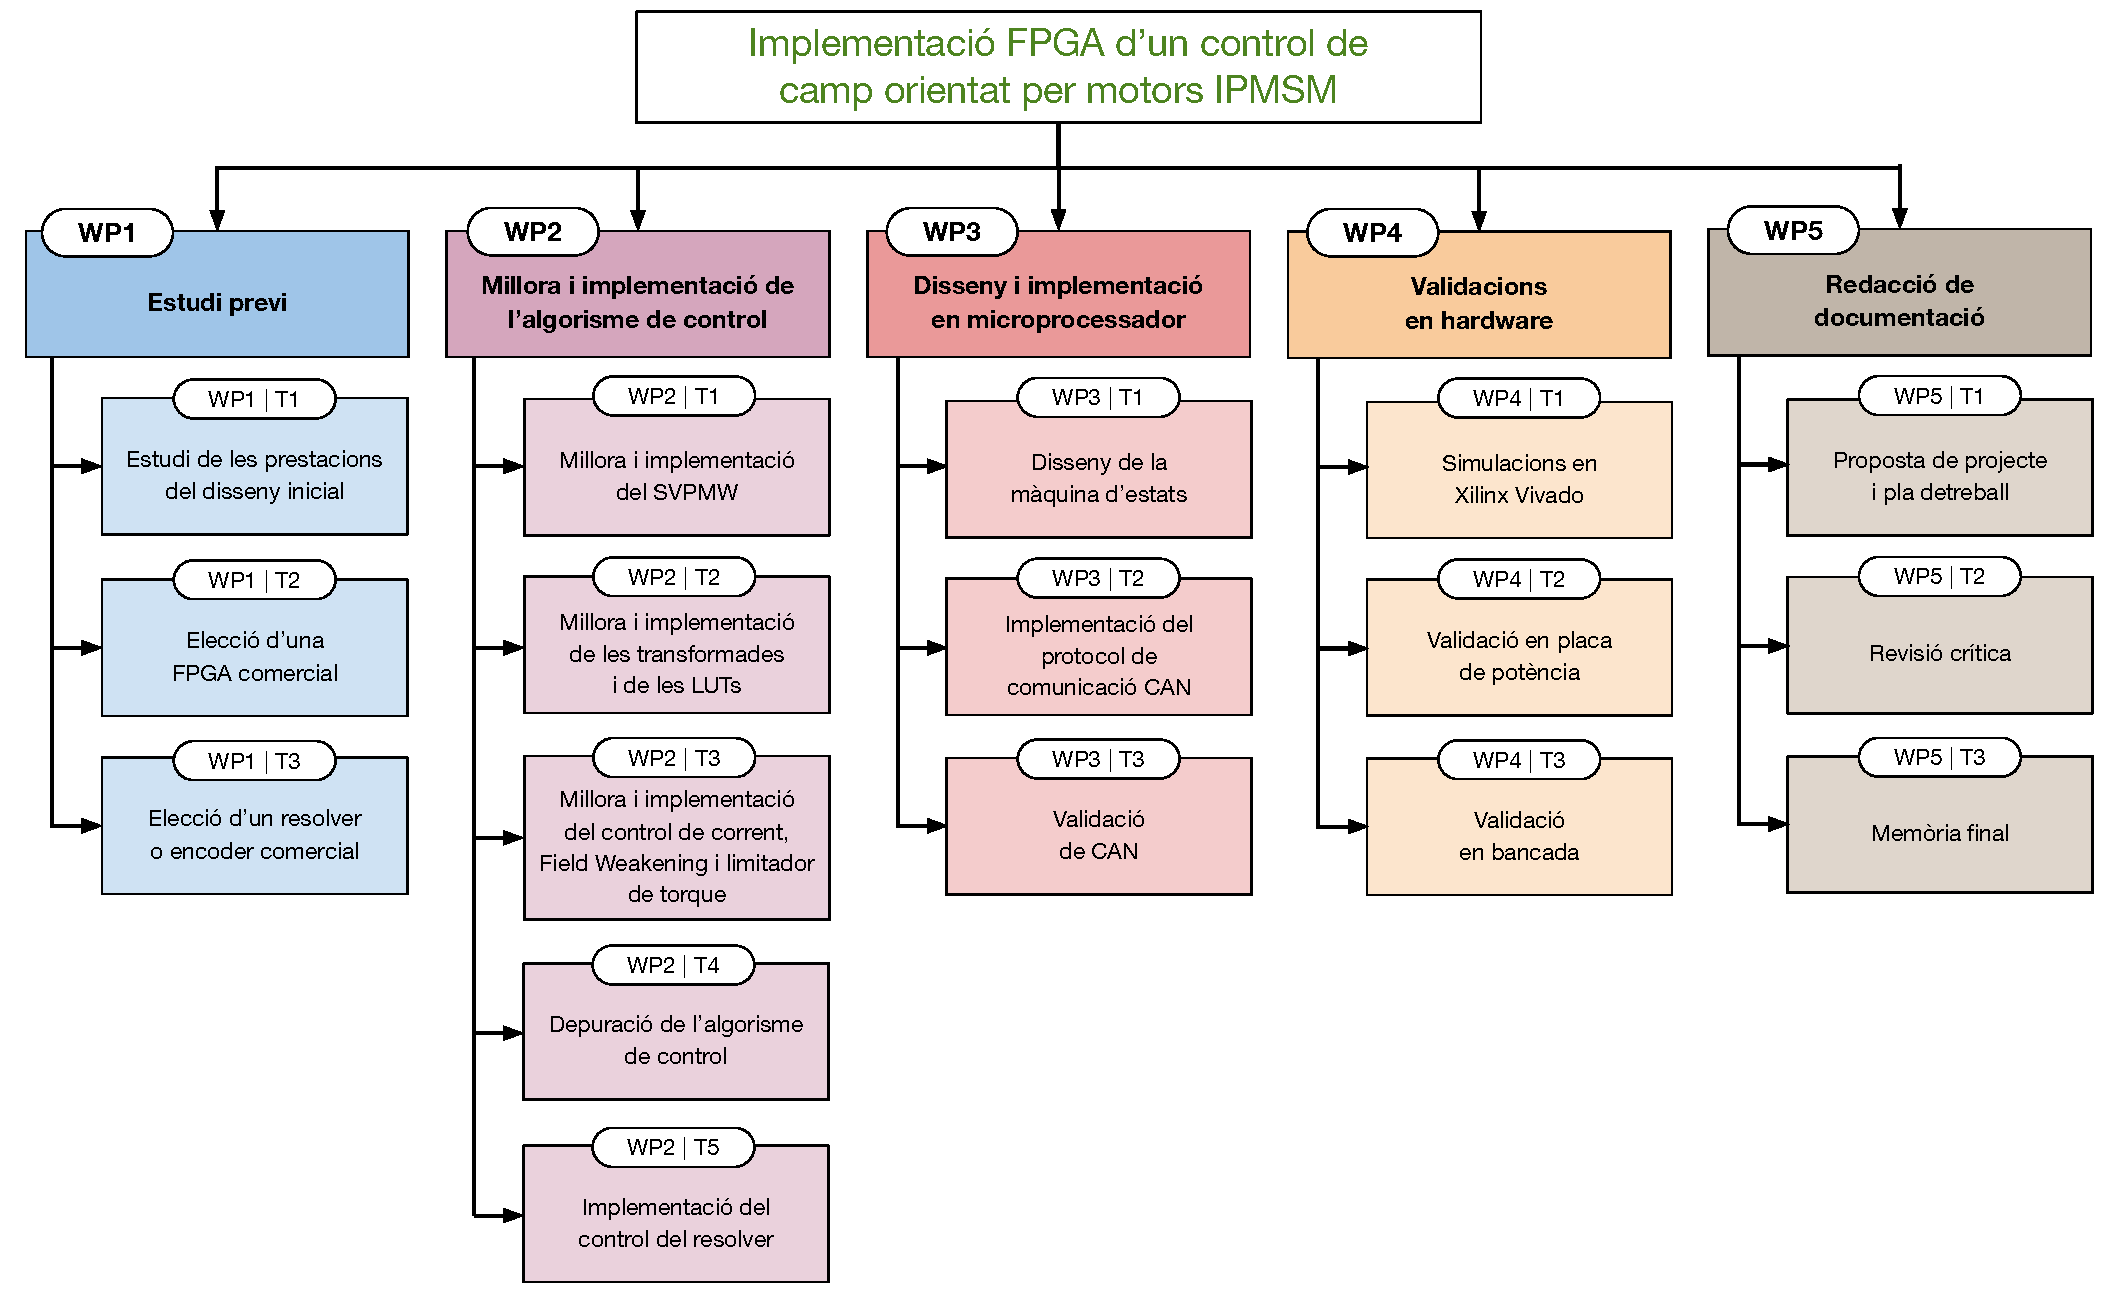
\includegraphics[width=15cm]
                { img/introduccio/wbs.pdf }
            \caption{ Work Breakdown Structure. }
        \end{figure}

        \newcounter{wpref}
\renewcommand{\arraystretch}{1.25}


% ----------------------------------------------------------------------
% WP1

\stepcounter{wpref}
\begin{center}
    \begin{tabular}{| p{8.5cm} | p{5.25cm} |}
        \hline
            \textbf{WP name:} 
                \newline \hspace*{0.3cm}
                \begin{minipage}[t]{8cm}
                    Estudi i investigació prèvia
                \end{minipage}
                \smallskip
            & 
            \textbf{WP ref:} 
                \newline \hspace*{0.3cm}
                \begin{minipage}[t]{8cm}
                    \arabic{wpref}
                \end{minipage}
            \\
        \hline
            \textbf{Short description:} 
                \newline \hspace*{0.3cm}
                \begin{minipage}[t]{8cm}
                    En aquest paquet de treball, es realitza un estudi de les
                    prestacions del disseny elaborat per l'equip amb l’objectiu
                    de trobar les seves deficiències i proposar millores o
                    redissenys que incrementin la qualitat del control.
                    Mentrestant, es realitza una investigació per a l’elecció
                    d’una placa FPGA en la qual implementar l’algorisme de
                    control i un resolver o encoder.
                \end{minipage}
                \smallskip
            &
            \textbf{Planned start date:} \newline \hspace*{0.3cm} 
                { 14/03/2022 } \newline
            \textbf{Planned end date:} \newline \hspace*{0.3cm} 
                { 23/04/2022 } \\
        \hline

            \textbf{Internal task T1:} 
                \newline \hspace*{0.3cm}
                \begin{minipage}[t]{8cm}
                    Estudi de les prestacions del disseny inicial
                \end{minipage}
                \smallskip

            \textbf{Internal task T2:} 
                \newline \hspace*{0.3cm}
                \begin{minipage}[t]{8cm}
                    Elecció d’una placa FPGA comercial
                \end{minipage}
                \smallskip

            \textbf{Internal task T3:}
                \newline \hspace*{0.3cm}
                \begin{minipage}[t]{8cm}
                    Elecció d’un resolver o encoder comercial
                \end{minipage}
                \smallskip
            & 
            \textbf{ Deliverables: }
                \begin{itemize}
                    \item { Model en Simulink (.xls) }
                    \item { Figures comentades generades per simulació }
                    \item { Fitxers VHDL (.hdl) }
                \end{itemize} \\
        \hline
    \end{tabular}
\end{center}


% ----------------------------------------------------------------------
% WP2 

\stepcounter{wpref}
\begin{center}
    \begin{tabular}{| p{8.5cm} | p{5.25cm} |}
        \hline
            \textbf{WP name:} 
                \newline \hspace*{0.3cm}
                \begin{minipage}[t]{8cm}
                    Impementació de l'algorisme
                \end{minipage}
                \smallskip
            & 
            \textbf{WP ref:}
                \newline \hspace*{0.3cm}
                \begin{minipage}[t]{8cm}
                    \arabic{wpref}
                \end{minipage}
            \\
        \hline
            \textbf{Short description:} 
                \newline \hspace*{0.3cm}
                \begin{minipage}[t]{8cm}
                    Aquest paquet de treball consisteix a realitzar el
                    redisseny (si escau) i la implementació, primer en Simulink
                    i després en codi VHDL, de l’algorisme de control.
                \end{minipage}
                \smallskip
            &
            \textbf{Planned start date:} \newline \hspace*{0.3cm} 
                { 28/02/2022 } \newline
            \textbf{Planned end date:} \newline \hspace*{0.3cm} 
                { 13/03/2022 } \\
        \hline

            \textbf{Internal task T1:} 
                \newline \hspace*{0.3cm}
                \begin{minipage}[t]{8cm}
                    Millora i implementació del SVPWM 
                \end{minipage}
                \smallskip

            \textbf{Internal task T2:} 
                \newline \hspace*{0.3cm}
                \begin{minipage}[t]{8cm}
                    Millora i implementació de les transformades de Clarke, de
                    Park i de Park inversa, i de les LUTs del sinus, del
                    cosinus, de l’arrel quadrada i de l’arrel quadrada
                    recíproca
                \end{minipage}
                \smallskip

            \textbf{Internal task T3:}
                \newline \hspace*{0.3cm}
                \begin{minipage}[t]{8cm}
                    Millora i implementació dels controls PI per al control del
                    corrent, Field Weakening i el limitador de torque
                \end{minipage}
                \smallskip

            \textbf{Internal task T4:} 
                \newline \hspace*{0.3cm}
                \begin{minipage}[t]{8cm}
                    Depuració del sistema complet
                \end{minipage}
                \smallskip

            \textbf{Internal task T5:}
                \newline \hspace*{0.3cm}
                \begin{minipage}[t]{8cm}
                    Millora i implementació del control del resolver
                \end{minipage}
                \smallskip
            &
            \textbf{ Deliverables: }
                \begin{itemize}
                    \item { Figures comentades generades per simulació }
                    \item { Taules comparatives }
                \end{itemize} \\
        \hline
    \end{tabular}
\end{center}


% ----------------------------------------------------------------------
% WP3 

\stepcounter{wpref}
\begin{center}
    \begin{tabular}{| p{8.5cm} | p{5.25cm} |}
        \hline
            \textbf{WP name:}
                \newline \hspace*{0.3cm}
                \begin{minipage}[t]{8cm}
                    Disseny i implementació en microprocessador 
                \end{minipage}
                \smallskip
            & 
            \textbf{WP ref:}
                \newline \hspace*{0.3cm}
                \begin{minipage}[t]{8cm}
                    \arabic{wpref}
                \end{minipage}
            \\
        \hline
            \textbf{Short description:} 
                \newline \hspace*{0.3cm}
                \begin{minipage}[t]{8cm}
                    Aquest paquet de treball consisteix a dissenyar,
                    implementar i validar la gestió de la comunicació i altres
                    interrupcions i events sobre el microcontrolador que
                    incorpora la placa FPGA.
                \end{minipage}
                \smallskip
            &
            \textbf{Planned start date:} \newline \hspace*{0.3cm} 
                { 22/04/2022 } \newline
            \textbf{Planned end date:} \newline \hspace*{0.3cm} 
                { 10/05/2022 } \\
        \hline

            \textbf{Internal task T1:} 
                \newline \hspace*{0.3cm}
                \begin{minipage}[t]{8cm}
                    Disseny de la màquina d’estats
                \end{minipage}
                \smallskip

            \textbf{Internal task T2:} 
                \newline \hspace*{0.3cm}
                \begin{minipage}[t]{8cm}
                    Implementació del protocol de comunicació CAN
                \end{minipage}
                \smallskip

            \textbf{Internal task T3:}
                \newline \hspace*{0.3cm}
                \begin{minipage}[t]{8cm}
                    Validació amb un CAN bus analyzer
                \end{minipage}
                \smallskip
            & 
            \textbf{ Deliverables: }
                \begin{itemize}
                    \item { Diagrama d’estats }
                    \item { Codi en C de la màquina d’estats }
                    \item { Captures de les trames de comunicació }
                \end{itemize} \\
        \hline
    \end{tabular}
\end{center}


% ----------------------------------------------------------------------
% WP4 

\stepcounter{wpref}
\begin{center}
    \begin{tabular}{| p{8.5cm} | p{5.25cm} |}
        \hline
            \textbf{WP name:} 
                \newline \hspace*{0.3cm}
                \begin{minipage}[t]{8cm}
                    Validació de l’algorisme de control en hardware
                \end{minipage}
                \smallskip
                \newline
            & 
            \textbf{WP ref:} 
                \newline \hspace*{0.3cm}
                \begin{minipage}[t]{8cm}
                    \arabic{wpref}
                \end{minipage}
            \\
        \hline
            \textbf{Short description:} 
                \newline \hspace*{0.3cm}
                \begin{minipage}[t]{8cm}
                    En aquest paquet de treball, es validaran les prestacions
                    de l’algorisme de control implementat. La validació es durà
                    a terme en tres fases: una primera en què se simula l’àrea
                    utilitzada i la temportizació mitjançant Vivado, el
                    software del fabricant Xilinx per al desenvolupament amb
                    FPGAs; una segona fase consistent en la validació sobre la
                    placa de potència i finalment una validació en bancada en
                    la que es posa a prova el control dels motors.
                \end{minipage}
                \smallskip
            &
            \textbf{Planned start date:} \newline \hspace*{0.3cm} 
                { 11/05/2022 } \newline
            \textbf{Planned end date:} \newline \hspace*{0.3cm} 
                { 08/06/2022 } \\
        \hline

            \textbf{Internal task T1:} 
                \newline \hspace*{0.3cm}
                \begin{minipage}[t]{8cm}
                    Simulacions en Xilinx Vivado
                \end{minipage}
                \smallskip

            \textbf{Internal task T2:} 
                \newline \hspace*{0.3cm}
                \begin{minipage}[t]{8cm}
                    Validació en placa de potència
                \end{minipage}
                \smallskip

            \textbf{Internal task T3:}
                \newline \hspace*{0.3cm}
                \begin{minipage}[t]{8cm}
                    Validació en bancada
                \end{minipage}
                \smallskip
            & 
            \textbf{ Deliverables: }
                \begin{itemize}
                    \item { Captures de la simulació }
                    \item { Informes autogenerats d'utilització i de temporització }
                    \item { Imatge d'arrencada en targeta SD (extensió .bin) }
                    \item { Captrues del monitors dels instruments de testeig }
                \end{itemize} \\
        \hline
    \end{tabular}
\end{center}


% ----------------------------------------------------------------------
% WP5 %

\stepcounter{wpref}
\begin{center}
    \begin{tabular}{| p{8.5cm} | p{5.25cm} |}
        \hline
            \textbf{WP name:} 
                \newline \hspace*{0.3cm}
                \begin{minipage}[t]{8cm}
                    Redacció de la documentació
                \end{minipage}
                \smallskip
            & 
            \textbf{WP ref:} 
                \newline \hspace*{0.3cm}
                \begin{minipage}[t]{8cm}
                    \arabic{wpref}
                \end{minipage}
            \\
        \hline
            \textbf{Short description:} 
                \newline \hspace*{0.3cm}
                \begin{minipage}[t]{8cm}
                    Aquest bloc de treball consisteix a recopilar el
                    coneixement generat, ordenar-lo i redactar la documentació
                    requerida.
                \end{minipage}
                \smallskip
            &
            \textbf{Planned start date:} \newline \hspace*{0.3cm} 
                { 28/02/2022 } \newline
            \textbf{Planned end date:} \newline \hspace*{0.3cm} 
                { 19/06/2022 } \\
        \hline

            \textbf{Internal task T1:} 
                \newline \hspace*{0.3cm}
                \begin{minipage}[t]{8cm}
                    Redacció de la proposta de projecte i pla de treball
                \end{minipage}
                \smallskip

            \textbf{Internal task T2:} 
                \newline \hspace*{0.3cm}
                \begin{minipage}[t]{8cm}
                    Redacció de la revisió crítica
                \end{minipage}
                \smallskip

            \textbf{Internal task T3:}
                \newline \hspace*{0.3cm}
                \begin{minipage}[t]{8cm}
                    Redacció de la memòria final
                \end{minipage}
                \smallskip
            & 
            \textbf{Deliverables: }
                \begin{itemize}
                    \item { Proposta de projecte i pla de treball }
                    \item { Revisió crítica }
                    \item { Memòria final }
                \end{itemize} \\
        \hline
    \end{tabular}
\end{center}

    }

    \subsubsection { Fites i lliurables }
    {
        En aquest apartat s'adjunta una taula amb les fites a assolir i els
        lliurables corresponents, ordenats temporalment i classificats per bloc
        de treball i tasques pertanyents.

        \begin{table}[!htb]
            \caption{ Taula de fites i lliurables }
            \centering
            \tablefirsthead{}
            \tablehead{}
            \tabletail{}
            \tablelasttail{}
            \renewcommand{\arraystretch}{1.3}

            \begin{supertabular}{|m{1.1cm}|m{1.8cm}|m{4.3cm}|m{4.3cm}|m{2.4cm}|}
                \hline
                    \textbf{ WP\# } & 
                    \textbf{ Tasques } & 
                    \textbf{ Títol curt } & 
                    \textbf{ Fita o lliurable } & 
                    \textbf{ Data } \\
                \hline
                    { 5 } & 
                    { 1 } & 
                    { Redacció de la propsota de projecte i pla de treball } & 
                    { Proposta de treball } & 
                    { Setmana 2 (07/02/2022) } \\
                \hline
                    { 1 } & 
                    { 1 } & 
                    { Estudi de les prestacions del disseny inicial } & 
                    { Document amb els resultats de les simulacions comentats } & 
                    { Setmana 2 (13/02/2022) } \\
                \hline
                    { 2 } & 
                    { 1, 2, 3, 4, 5 } & 
                    { Millora i implementació de l'algorisme de control } & 
                    { Document amb els resultats de les simulacions comentats } & 
                    { Setmana 8 (23/04/2022) } \\
                \hline
                    { 5 } &
                    { 2 } & 
                    { Redacció de la revisió crítica } & 
                    { Revisió crítica} & 
                    { Setmana 8 (22/04/2022) } \\
                \hline
                    { 3 } & 
                    { 1 } & 
                    { Disseny de la màquina d'estats } & 
                    { Diagrama d'estats } & 
                    { Setmana 9 (27/04/2022) } \\
                \hline
                    { 3 } & 
                    { 2, 3 } & 
                    { Implementació i validació del protocol CAN } & 
                    { Document amb les trames de comunicació comentades } & 
                    { Setmana 11 (10/05/2022) } \\
                \hline
                    { 4 } & 
                    { 1 } & 
                    { Simulacions amb Vivado de Xilinx } & 
                    { Document amb els resultats de les simulacions comentats } & 
                    { Setmana 11 (15/05/2022) } \\
                \hline
                    { 4 } & 
                    { 2 } & 
                    { Validació en placa de potència } & 
                    { Document amb les figures obtingudes comentades } & 
                    { Setmana 13 (26/05/2022) } \\
                \hline
                    { 4 } & 
                    { 3 } & 
                    { Validació en bancada } & 
                    { Document amb les figures obtingudes comentades } & 
                    { Setmana 15 (08/06/2022) } \\
                \hline
                    { 5 } & 
                    { 3 } & 
                    { Redacció de la memòria } & 
                    { Memòria final } & 
                    { Setmana 17 (21/06/2022) } \\
                \hline
            \end{supertabular}
        \end{table}
    }

    \subsubsection { Diagrama de Gantt }
    {
        A continuació d'adjunta el diagrama de Gantt el projecte, on es pot
        veure l'evolució en el temps de les tasques. \clearpage

        \begin{figure}[!htb]
            \centering
            \begin{ganttchart}[
    y unit title = 0.4cm,
    y unit chart = 0.5cm,
    vgrid, 
    hgrid,
    title height = 1,
    today = 17,
    today offset = .5,
    today label = Now,
    bar/.style = { draw, fill = cyan },
    bar incomplete/.append style = { fill = yellow!50 },
    bar height=0.7
]{1}{17}

% dies
\gantttitle{Fases del projecte}{17} \\
\gantttitle{Març}{5}
\gantttitle{Abril}{4}
\gantttitle{Maig}{4}
\gantttitle{Juny}{4} \\
 
% caixes elem0 .. elem9 
\ganttgroup[inline=false]{Treball previ}{1}{2}\\
    \ganttbar[progress=100]{Estudi del disseny inicial}{1}{2} \\
    \ganttbar[progress=100]{Elecció de la FPGA}{1}{1} \\
    \ganttbar[progress=100]{ Elecció de resolver o encoder }{2}{2} \\ \\
 
\ganttgroup[inline=false]{Algorisme de control}{3}{8}\\
    \ganttbar[progress=100]{ Impl. de SVPWM }{3}{3} \\
    \ganttbar[progress=100]{ Impl. de transformades i LUTs }{4}{4} \\
    \ganttbar[progress=100]{ Impl. del ctrl. de corrent, FW i altres }{5}{5} \\
    \ganttbar[progress=100]{ Depuració de l'algorisme de control }{6}{7} \\
    \ganttbar[progress=100]{ Control del resolver }{8}{8} \\ \\
 
\ganttgroup[inline=false]{Microprocessador}{9}{11}\\
    \ganttbar[progress=100]{ Disseny de la màquina d'estats }{9}{9} \\
    \ganttbar[progress=100]{ Implementació de CAN }{10}{10} \\
    \ganttbar[progress=0]{ Validació de CAN }{11}{11} \\ \\
 
\ganttgroup[inline=false]{Simulacions i validacions}{12}{15}\\
    \ganttbar[progress=100]{Simulació en Xilinx Vivado}{12}{12} \\
    \ganttbar[progress=0]{Validació en placa de potència}{13}{13} \\
    \ganttbar[progress=0]{Validadió en bancada}{14}{15} \\ \\
 
\ganttgroup[inline=false]{Documentació i lliurables}{1}{16}\\
    \ganttbar[progress=100]{Redacció de la proposta de treball}{1}{1} \\
    \ganttmilestone{Lliurament de la proposta de treball}{1}{1} \\
    \ganttbar[progress=100]{Redacció de la revisió crítica}{7}{8} \\
    \ganttmilestone{Lliurament de la proposta de treball}{8}{8} \\
    \ganttbar[progress=100]{Redacció de la memòria final}{10}{16} \\
    \ganttmilestone{Lliurament de la proposta de treball}{16}{16} \\ \\

\end{ganttchart}

            \caption{ Diagrama de Gantt del projecte }
        \end{figure}
    }

    \subsubsection { Supervisió del projecte }
    {
        S'ha realitzat una reunió semanal amb el supervisor del projecte,
        l'horari de la qual es convenia amb segons la seva disponibilitat.

        A part de les reunions de supervisió general, s'han realitzat tres
        reunions en les dates següents:

        \begin{table}[!htb]
            \caption{ Pla de supervisió del projecte }
            \centering
            \tablefirsthead{}
            \tablehead{}
            \tabletail{}
            \tablelasttail{}

            \begin{supertabular}{|m{10cm}|m{4cm}|}
                \hline
                    \textbf{Reunió} & \textbf{Data} \\
                \hline
                    { Revisió de la proposta de projecte i pla de treball }
                    & { 04/03/2022 } \\
                \hline
                    { Revisió del document de revisió crítica }
                    & { 18/04/2022 } \\
                \hline
                    { Revisió de la memòria final }
                    & { 21/06/2022 } \\
                \hline
            \end{supertabular}
        \end{table}
    }

    \subsubsection { Incidències i desviació del pla de treball original }
    {
        La primera part del projecte es va executar sense gaires problemes.
        S'hi destaca una lleugera dificultat a l'hora de depurar l'algorisme de
        control amb el blockset de Vitis Model Composer en Simulink. En
        conseqüència, els terminis van quedar bastant ajustats, situant-me
        just a temps o uns dies per darrere del pla de treball original.

        Tanmateix, la segona part del projecte es va desenvolupar d'una
        manera més accidentada. En primer lloc, s'hi destaca el retràs en la
        comanda de la FPGA, la qual cosa ha fet bastant difícil que es validès
        el CAN. Es va provar a simular el CAN en la placa FPGA que ja disposava
        l'equip sense èxit, degut a problemes de compatibilitat de les eines
        per instalar Linux.
    }
}

\subsection { Continguts de la memòria }
{
    \subsubsection*{ Capítol 1 - Introducció }
    {
        Aquest primer capítol ha consistit en una introducció al projecte i la
        seva importància, així com la presentació dels objectius,
        especificacions, mètodes, procediments i pla de treball seguits en el
        desenvolupament del projecte.
    }

    \subsubsection*{ Capítol 2 - Formula Student i tren de potència }
    {
        En el segon capítol es realitza una contextualització del projecte de
        l'inversor propi dins de la competició de Formula Student i la seva
        importància per l'equip de BCN eMotorsport. 
        
        També es descriu la configuració del tren de potència en el vehicle de
        l'equip, justificant els aspectes tinguts en compte a l'hora de
        plantejar el projecte.
    }

    \subsubsection*{ Capítol 3 - Estudi teòric del control motor }
    {
        En aquest tercer capítol es presenta el desenvolupament teòric del
        control i s'analitza el model realitzat pels membres de l'equip, previ
        a la implementació a realitzar en \ac{FPGA}.
    }

    \subsubsection*{ Capítol 4 - Disseny i implementació }
    {
        En el quart capítol es conduirà el lector pel procés de disseny de la
        proposta d'implementació i el desenvolupament de la mateixa. Es
        començarà justificant les decisions presses i es continuarà anlitzant
        l'estructura final de la implementació, tant a nivell de lògica
        programable com de programació del microprocessador.
    }
    
    \subsubsection*{ Capítol 5 - Experiments i resultats }
    {
        En aquest capítol s'exposaran els experiments realitzats per validar la
        implementació i s'analitzaran els resultats obtinguts.
    }
    
    \subsubsection*{ Capítol 6 - Estudi econòmic }
    {
        En el capítol 6 es despleguen i s'estimen els costos del projecte.
    }
    
    \subsubsection*{ Capítol 7 - Conclusions }
    {
        En la conclusió es valora l'evolució del projecte, es posaran en valor
        els resultats obtinguts i s'hi realitzarà una crítica a la metodologia
        utilitzada i a altres aspectes de desenvolupament durant el projecte.
    }
    
    \subsubsection*{ Capítol 8 - Treball futur }
    {
        Per últim, en el captítol 8 s'exposaran els passos que es realitzaran
        després d'acabar el projecte.
    }
}

\clearpage \section{Formula Student i tren de potència}
\subsection{ Introducció a la Formula Student }
{
    La Formula Student és una sèrie de competicions automovilístiques en la que
    participen equips formats per estudiants universitaris arran el món. La
    competició consisteix a dissenyar i construir un vehicle monoplaça, i té
    com objectiu final promoure l'excelència entre els estudiants d'enginyeria.
    D'aquesta manera no es valoren només els resultats esportius, sino també
    les capacitats tècniques, la justificació del disseny i la viabilitat
    empresarial de la proposta de negoci que s'elabora de forma paral·lela.

    \begin{figure}[!htb]
        \centering
        \captionsetup{justification=centering,margin=1.5cm}
        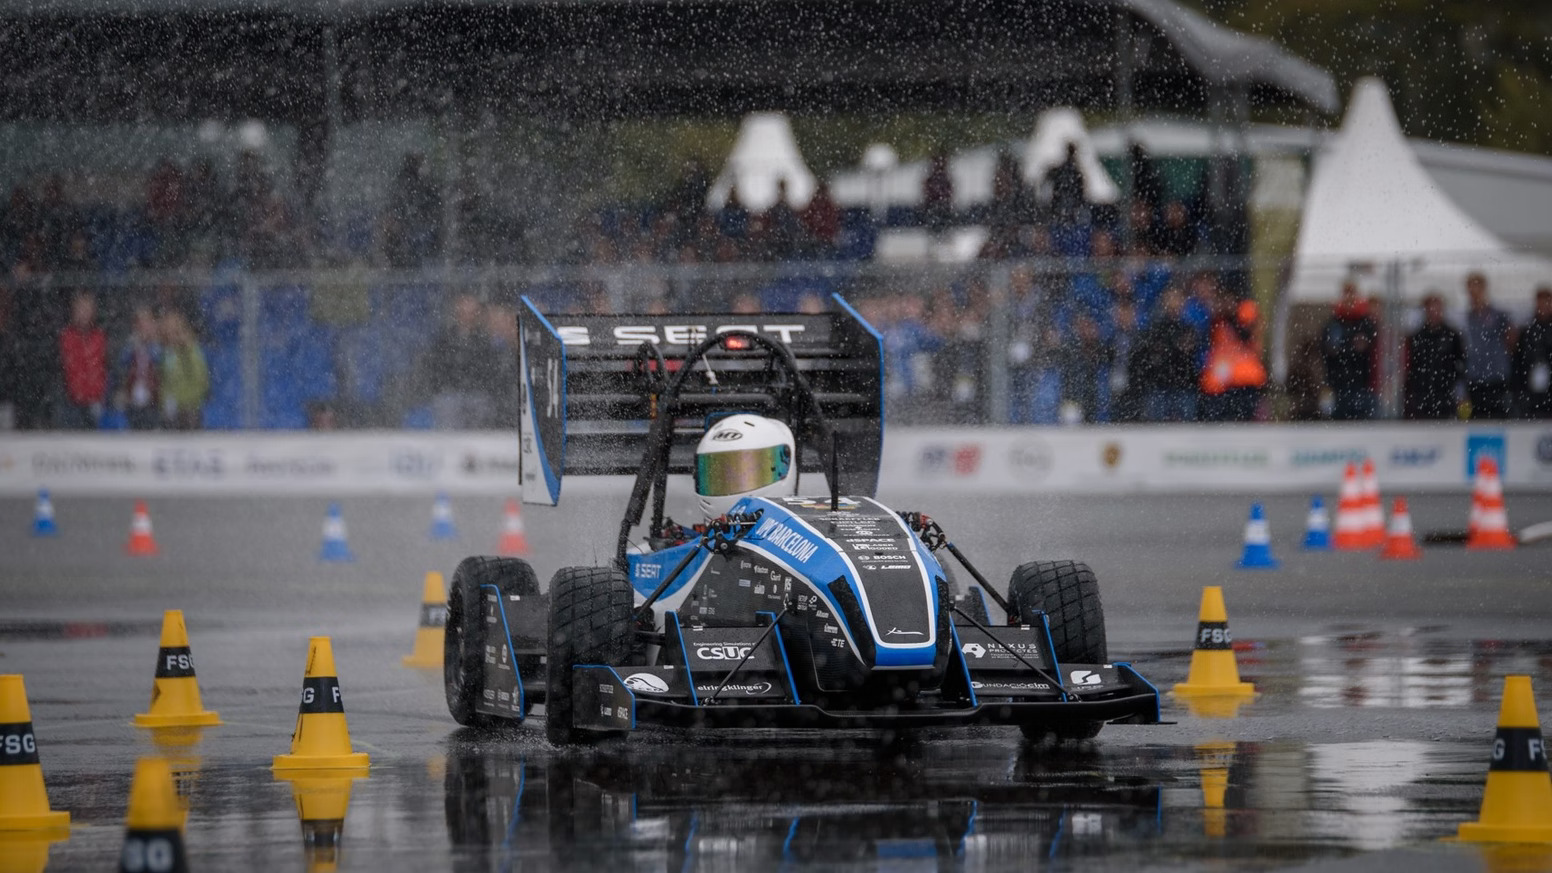
\includegraphics[width=8cm]
            { img/2_formula_student/foto_guay.jpg } 
        \caption[Competició de Formula Student. \emph{BCN eMototsport}]
        { 
            Vehicle de l'equip BCN eMotorsport durant una prova de
            Formula Student. \emph{BCN eMototsport} 
        }
    \end{figure}
    
    La Formula Student va néixer el 1979 de la mà de Mark Marshek, docent de la
    Universitat de Houston, quan va presentar la idea de realitzar competicions
    universitàries d'enginyeria al departament de Relacions Educatives de la
    \ac{SAE}. Poc després, al 1981, es va realitzar la primera edició de la
    Formula \ac{SAE}, en la qual participaren 6 equips formats per uns 40
    estudiants.\cite{formula_student}

    La Formula Student ha anat adaptant-se als avenços tecnològics de les
    últimes dècades. Així, el 2010 es va començar a introduir la mobilitat
    elèctrica, incorporant-se a la competició com una nova categoria. D'altra
    banda, el 2016 es va crear la categoria \emph{Driverless} per donar cabuda
    al desenvolupament de la tecnologia de conducció autònoma.

    Actualment, existeixen més de 700 equips de Formula Student que participen
    en els 17 esdeveniments de Formula Student que tenen lloc al voltant del
    món.
}

\subsection{ BCN eMotorsport }
{
    BCN eMotorsport és l'equip que representa les escoles d'enginyeria de
    l'\ac{ETSEIB} i l'\ac{ETSETB} a les competicions de Formula Student. Cada
    any l'equip dissenya, fabrica i testeja un vehicle monoplaça de competició.

    L'equip és fundat el 2007 per 13 estudiants de l'\ac{ETSEIB}, adoptant el
    nom de \emph{\ac{ETSEIB} Motorsport} i convertint-se en un dels primers
    equips de Formula Student d'Espanya. En aquell precís moment els seus
    membres comencen a treballar en el prototip del seu primer vehicle, el
    CAT01, de combustió interna. L'any 2008 \emph{\ac{ETSEIB} Motorsport}
    participa en la seva primera competició de Formula Student. El 2011,
    l'equip va començar a competir en categoria elèctrica, sent el primer equip
    espanyol en fer-ho. Tots els vehicles posteriors han continuat sent
    elèctrics.

    D'altra banda, l'any 2018 sorgeix un nou projecte a l'\ac{ETSETB} el primer
    equip espanyol en participar en categoria autònoma, \emph{Driverless UPC}.
    Dos anys després, al 2020, es produeix la fusió dels equips de
    \emph{\ac{ETSEIB} Motorsport} i \emph{Driverless UPC}, donant lloc a
    l'equip actual de \emph{BCN eMotorsport}. \cite{bcn_emotorsport}

    Any rere any l'equip afegeix innovacions tècniques per millorar el
    rendiment del vehicle i els resultats a les competicions, entre altres, la
    implementació de l'algorisme de Torque Vectoring per la tracció a quatre
    rodes, la incorporació de frenada regenerativa o un algorisme de State of
    Charge per estimar el nivell de bateria. Aquest any l'equip compleix 15
    anys i uns dels projectes que ha pres més força és el projecte de
    l'inversor propi.

    \begin{figure}[!htb]
        \centering
        \begin{minipage}[c]{7cm}
            \centering
            \captionsetup{justification=centering}
            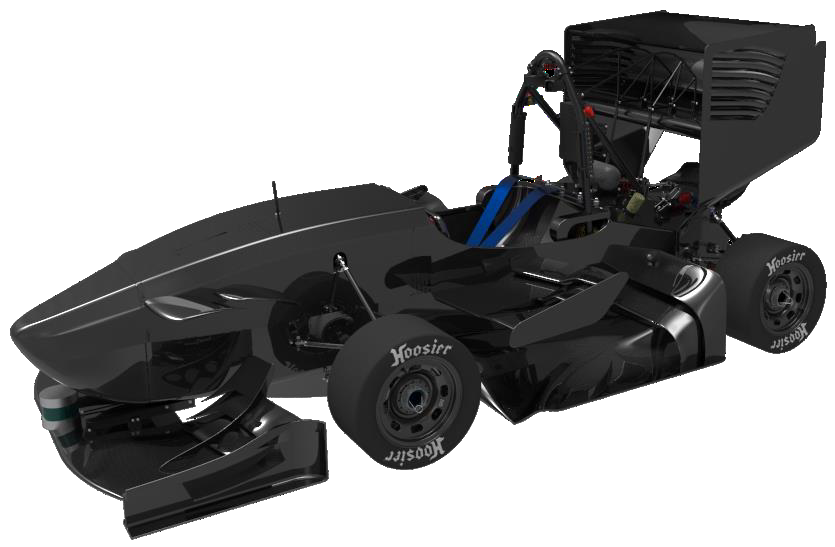
\includegraphics[width=7cm]
                { img/2_formula_student/cat14-x.png }
            \caption[Renderització del CAT14x. \emph{BCN eMotorsport} ]
            { 
                Renderització del vehicle de competició CAT14x d'aquesta
                temporada 2022. \emph{BCN eMotorsport.} 
            }             
        \end{minipage} \hfil
        \begin{minipage}[c]{7cm}
            \centering
            \captionsetup{justification=centering}
            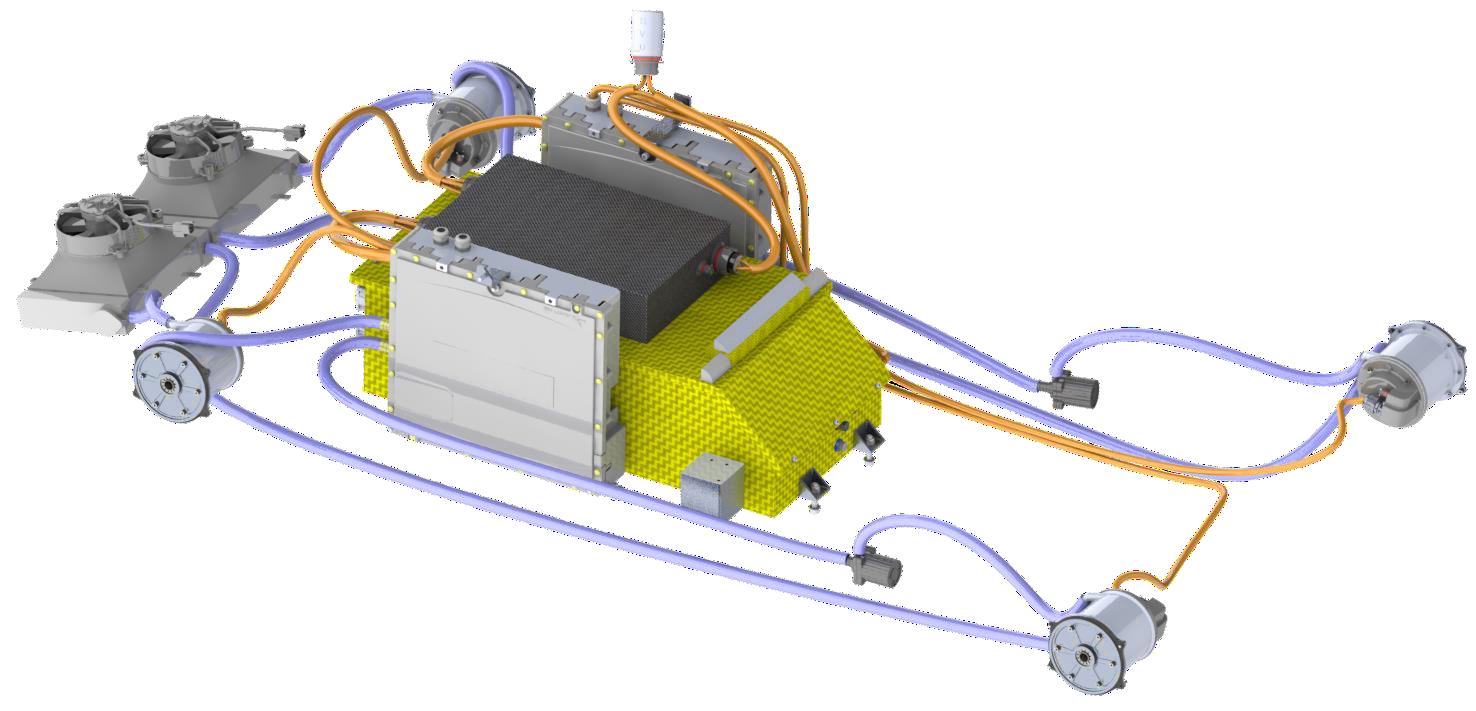
\includegraphics[width=7cm]
                { img/2_formula_student/power.png }
            \caption[Renderització del tren de potència. \emph{BCN eMotorsport} ]
            { 
                Renderització del model en SolidWorks del tren de potència.
                \emph{BCN eMotorsport.}  
            }                
        \end{minipage} \hfil
    \end{figure} 

    Els membres de l'equip es reparteixen en vuit seccions: aerodinàmica,
    chasis, control del vehicle, dinàmica del vehicle, percepció, electrònica,
    gestió i tren de potència. Cada una de les seccions s'encarrega del
    disseny, construcció i testeig d'una part del vehicle, a excepció de
    gestió, que s'encarrega d'elaborar el pla de negoci i gestionar el
    pressupost de l'equip.
}

\subsection{ Introducció al tren de potència }
{
    \begin{figure}[!htb]
        \centering
        \captionsetup{justification=centering, margin=1.5cm}
        
\includegraphics[width=13cm]
            { img/2_formula_student/power.pdf }
        \caption{ Esquema de connexió del tren de potència }
    \end{figure}

    El tren de potència d'un vehicle és el sistema encarregat d'emmagatzemar,
    transformar i entregar l'energia necessària per permetre la seva propulsió.
    En el cas d'un vehicle elèctric, aquest elements són la bateria, el motor,
    l'inversor, el cablejat i altres elements de seguretat. En els succesius
    vehicles elèctrics de l'equip, el tren de potència ha suposat habitualment
    entre el 45\% i el 50\% del seu pes, sent la bateria el component més
    pesat.

    \subsubsection{ Bateria }
    {
        Per reglament de la Formula Student, el voltatge màxim permès és de 600
        V \cite{fs_rules}. La capacitat de la bateria es dimensiona estudiant
        el consum d'energia del vehicle durant la prova de resistència
        (\emph{Endurance}), en la que el vehicle ha de recòrrer una distància
        de 22 km sense carregar les bateries \cite{sergio}. Compta amb un
        sistema de balanceig passiu per mitjà del \ac{BMS} i un circuit de
        precàrrega dels que limita el corrent durant la precàrrega dels
        condensadors de l'inversor, amb el qual és necessari communicar-se
        mitjançant CAN. Les especificacions de la bateria es recullen a la
        taula \ref{bateria}.

        \begin{figure}[!htb]
            \centering
            \captionsetup{justification=centering, margin=1.5cm}
            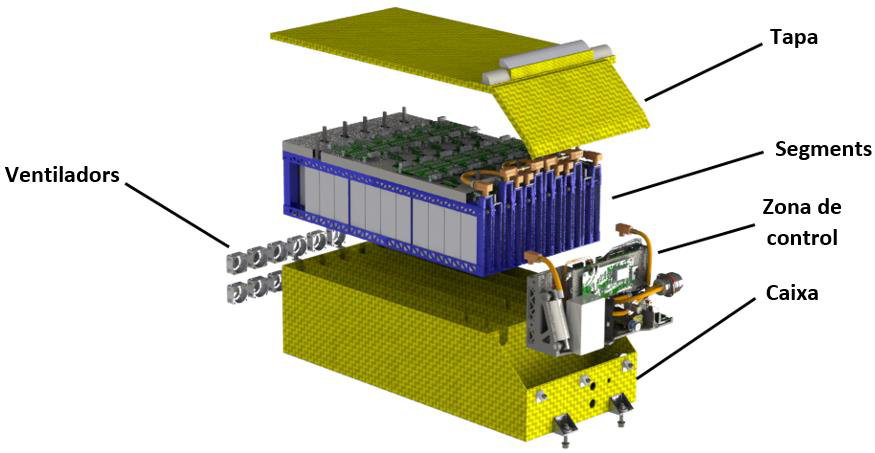
\includegraphics[width=9cm]
                { img/2_formula_student/bateria.png }
            \caption{ Bateria del CAT14x. \emph{BCN eMotorsport.}}
        \end{figure}

        \begin{table}[!htb]
            \caption{ Especificacions de la bateria del CAT14x }
            \label{bateria}
            \centering
            \renewcommand{\arraystretch}{1.3}
            \tablefirsthead{}
            \tablehead{}
            \tabletail{}
            \tablelasttail{}
        
            \begin{tabular}{|l|c|c|}
                \hline
                    \textbf{ Especificació } & 
                    \textbf{ Valor nominal } &
                    \textbf{ Valor màxim } \\
                \hhline{|=|=|=|}
                    { Voltatge total } & 
                        { $525,4 V$ } & 
                        { $596,4\ V$ } \\
                \hline
                    { Energia total } & 
                        { $7145,44\ Wh$ } & 
                        { $8111,04\ Wh$ } \\
                \hline
                    { Potència total } & 
                        { $15,4\ kW$ } & 
                        { $35,366\ kW$ } \\
                \hhline{|=|=|=|}
                    { Disposició de cel·les } & 
                        \multicolumn{2}{|c|}{ $142s2p$ } \\
                \hline
                    { Capacitat total } & 
                        \multicolumn{2}{|c|}{ $13,6\ Ah$ } \\
                \hline
                    { Pes } & 
                        \multicolumn{2}{|c|}{ $35,5\ kg$ } \\
                \hline
            \end{tabular}
        \end{table}
    }

    \subsubsection{ Motor }
    {
        Coneixem com motor elèctric aquell dispisitu capaç de convertir
        l'energia elèctrica en energia mecànica per mitjà de l'interacció
        d'elements capaços de generar i interactuar amb camps magnètics, com
        són els inductors i els imants. Un motor generalment consta de dues
        parts principals, l'estàtor i el rotor, que són la part fixa i la
        rotativa, respectivament. Entre els motors existents podem trobar
        motors que funcionen en continua o en alterna de tres fases o més;
        aquests últims, poden ser alhora síncrons o asíncrons (si la seva
        freqüència de rotació coincideix amb la freqüència de l'ona elèctrica
        que l'alimenta).
    
        El motor utilitzat per l'equip és un motor trifàsic síncron d'imants
        permanents interiors (\acs{IPMSM}). Aquest tipus de motor es
        carateritza per incorporar imants a l'interior del rotor, a diferència
        dels SPMSM, que els porten a la superfície del rotor. Els motors
        \acs{PMSM} són motors que admeten una densitat de potència molt
        elevada, en relació amb el seu pes i dimensions. A sobre, els motors
        IPMSM tenen una eficiencia una mica superior als SPMSM en aprofitar el
        parell de reluctància i poden assolir velocitats majors degut a que la
        tècnica de debilitament de camp (FW) és més apropiada amb imants
        permanents.

        \begin{figure}[!htb]
            \centering
            \captionsetup{justification=centering, margin=1.5cm}
            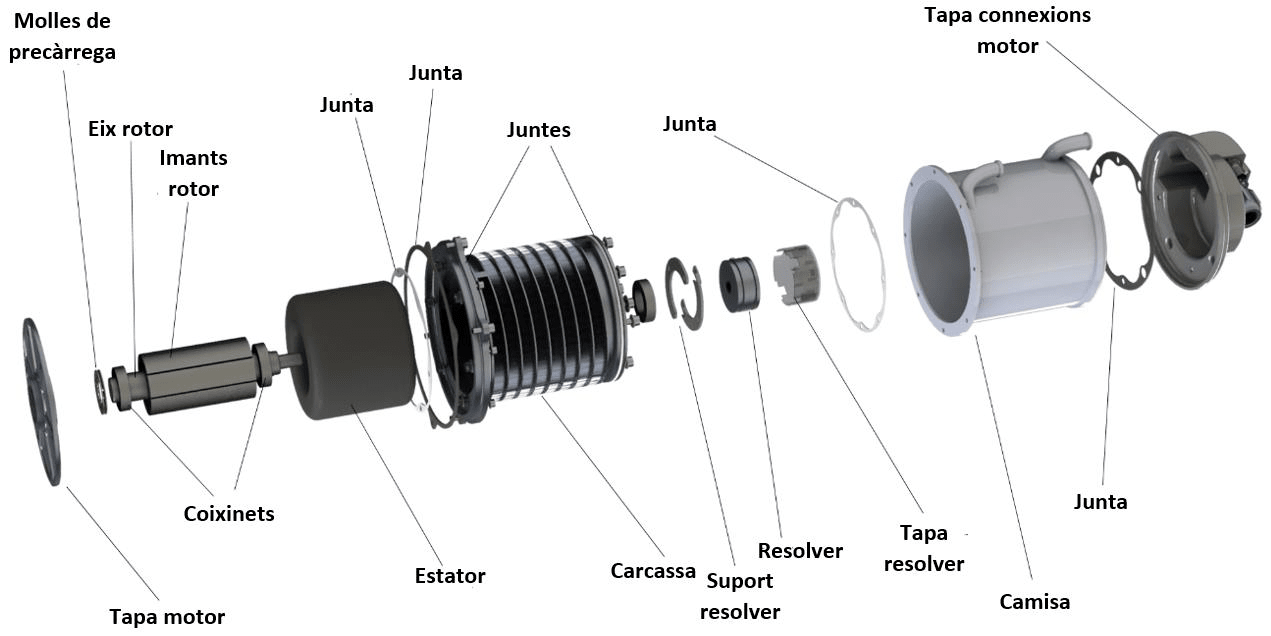
\includegraphics[width=10cm]
                { img/2_formula_student/motor.png }
            \caption{ Vista explosionada del motor del CAT14x. \emph{BCN eMotorsport.}}
        \end{figure}

        \begin{table}[!htb]
            \caption{ Fitxa tècnica del motor Fischer TI085-052-070-04B7S-07S04BE2 }
            \label{motor}
            \centering
            \renewcommand{\arraystretch}{1.3}
            \tablefirsthead{}
            \tablehead{}
            \tabletail{}
            \tablelasttail{}
        
            \begin{tabular}{|l|c|c|}
                \hline
                    \textbf{ Especificació } & 
                    \textbf{ Valor nominal } &
                    \textbf{ Valor màxim } \\
                \hhline{|=|=|=|}
                    { Parell } & 
                    { $11,1\ Nm$ } & 
                    { $29,1\ Nm$ } \\
                \hline
                    { Corrent eficaç } & 
                    { $22,6\ A_{rms}$ } & 
                    { $29,1\ A_{rms}$ } \\
                \hline
                    { Velocitat angular } & 
                    { $13250\ rpm$ } & 
                    { $20000\ rpm$ } \\
                \hline
                    { Potència } & 
                    { $15,4\ kW$ } & 
                    { $35,366\ kW$ } \\
                \hhline{|=|=|=|}
                    { Voltatge bus DC } & 
                    \multicolumn{2}{|c|}{ $600\ V$ } \\
                \hline
                    { Número de parells de pols } & 
                    \multicolumn{2}{|c|}{ 4 } \\
                \hline
                    { Resistència } & 
                    \multicolumn{2}{|c|}{ $0,126\ \Omega$ } \\
                \hline
                    { Inductància } & 
                    \multicolumn{2}{|c|}{ $0,393\ mH$ } \\
                \hline
                    { Tipus de connexió } & 
                    \multicolumn{2}{|c|}{ Estrella } \\
                \hline
                    { Velocitat al parell màxim } & 
                    \multicolumn{2}{|c|}{ $11600\ rpm$ } \\
                \hline
                    { Pes } & 
                    \multicolumn{2}{|c|}{ $4,5\ kg$ } \\
                \hline
            \end{tabular}
        \end{table}

        El CAT14x incorpora quatre motors IPMSM comercials de la marca
        \emph{Fischer Elektromotoren}, les especificacions del qual es
        resumeixen en la taula \ref{motor}. Disposar de quatre motors permet
        tenir tracció a quatre rodes (\emph{Four-wheel drive} o 4WD), la qual
        està controlada computacionalment per un algorisme de \emph{Torque
        Vectoring} desenvolupat per l'equip i implementat en la unitat de
        processament (\emph{Processing Unit}, PU) del vehicle.

        La mesura de l'angle del rotor respecte a l'estàtor es realitza
        actualment per mitjà de resolver. Es va barajar la idea de canviar d'un
        resolver a un encoder, però es decidí finalment continuar amb el
        resolver. Els resolvers són en general molt més robustos davant EMIs,
        ja que no disposen d'elements electrònics. No obstant, requereixen d'un
        circuit d'adequació, en el qual s'implementen amplificadors de senyal i
        algún sistema de detecció de l'angle i la velocitat angular, com
        pot ser un PLL (\emph{Phase Loocked Loop}). No obstant això, el
        requisit de fer intercanviable el nou inversor amb l'actual ha decantat
        la balança a favor del resolver.
    }

    \subsubsection{ Inversor }
    {
        Es coneix generalment com inversor, inversor de potència o ondulador al
        dispositiu encarregat de transferir potència d'una font de tensió
        continua a una càrrega de alterna. En el cas del vehicle de FS, la
        potència de la bateria es transfereix a cada un dels quatre motors per
        mitjà d'inversors.

        Els inversors que es fan servir per controlar la velocitat, el torque
        i/o la posició d'un motor es coneixen a la literatura com \emph{Motor
        Drive} (``conducció de motor''). En aquests casos es considera l'inversor
        com un component del \emph{Motor Drive}, en conjunció al motor, el
        sistema de control electrònic i els diversos sensors que tanquen el
        llaç de control.

        Els \emph{Motor Drives} que porta el vehicle d'aquesta temporada 2022,
        el CAT14x, són els doble inversors Lenze Mobile DSU 60/60, que porten
        dos inversors cadascun \cite{lenze}. Aquests inversors estan
        inicialment concebuts per la seva implementació en autobusos de tracció
        elèctrica i altres vehicles semblants destinats a la movilitat urbana.
        Es pot deduir, per tant, que es troba sobredimensionat per a la nostra
        aplicació particular d'un vehicle de competició que no sobrepassa els
        250 kg i està limitat a 80 kW de potència total per reglament
        \cite{fs_rules}.

        \begin{figure}[!htb]
            \centering
            \begin{minipage}[c]{7cm}
                \centering
                \captionsetup{justification=centering}
                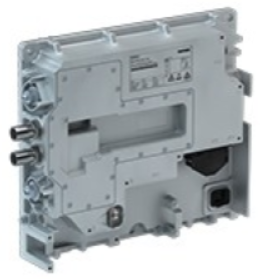
\includegraphics[width=5cm]
                { img/2_formula_student/inverter.png }
                \caption{ Doble inversor Lenze Mobile DSU 60/60. }
            \end{minipage} \hfil
            \begin{minipage}[c]{7cm}
                \centering
                \captionsetup{justification=centering}
                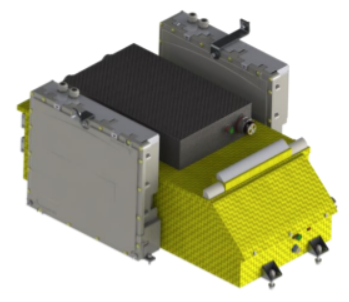
\includegraphics[width=5cm]
                { img/2_formula_student/inverter2.png } 
                \caption[ Col·locació dels Lenze Mobile ]
                { 
                    Col·locació dels dos Lenze Mobile DSU 60/60 respecte la
                    resta del tren de potència. \emph{BCN eMotorsport}
                }
            \end{minipage} \hfil
        \end{figure}

        \begin{table}[!htb]
            \caption{ Fitxa tècnica del doble inversor Lenze Mobile DSU 60/60 }
            \centering
            \renewcommand{\arraystretch}{1.3}
            \tablefirsthead{}
            \tablehead{}
            \tabletail{}
            \tablelasttail{}
        
            \begin{tabular}{|m{4cm}|c|c|c|}
                \hline
                    \textbf{ Especificació } & 
                    \textbf{ Mínima } &
                    \textbf{ Nominal } &
                    \textbf{ Màxima } \\
                \hhline{|=|=|=|=|}
                    { Voltatge bus DC } &
                    { $100\ V$ } &
                    { $800\ V$ } &
                    { $848\ V$ } \\
                \hline
                    { Tensió de sortida per fase } & 
                    { $0\ V$ } &
                    { - } & 
                    { $510\ V$ } \\
                \hline
                    { Freqüència de sortida } & 
                    { $-599\ Hz$ } & 
                    { - } & 
                    { $599\ Hz$ } \\
                \hline
                    { Corrent de curtcircuit a l'apagada } & 
                    { - } & 
                    { $96,2\ A$ } &
                    { - } \\
                \hline
                    { Consum de corrent } & 
                    { - } & 
                    { $39,2\ A$ } & 
                    { $70,5\ A$ } \\
                \hline
                    { Potència de sortida } & 
                    { - } & 
                    { $20\ kW$ } & 
                    { $36\ kW$ } \\
                \hline
                    { Corrent de sortida (segons conmutació) } & 
                    { $16\ A\ (16\ kHz)$ } & 
                    { $28,8\ A\ (8\ kHz)$ } &                    
                    { $51,2\ A\ (2\ kHz)$ } \\
                \hhline{|=|=|=|=|}
                    { Pes } & 
                    \multicolumn{3}{|c|}{ $7,4\ kg$ } \\
                \hline
                    { Dimensions } & 
                    \multicolumn{3}{|c|}{ $310,6 mm \times 354,5 mm \times 75 mm$ } \\
                \hline
            \end{tabular}
        \end{table}

        El projecte de l'inversor propi apareix com alternativa a l'inversor
        Lenze Mobile DSU 60/60. Com s'ha comentat, l'inversor es troba
        sobredimensionat respecte les característiques del vehicle; no obstant,
        aquest no és l'únic desavantatge. 
        
        Tenim per un costat que el funcionament intern dels Lenze és totalment
        desconegut per l'equip. El fabricant aporta documentació respecte a
        l'interfície de comunicació i els modes de funcionament, però no acaba
        d'explicar com aprofitar el rendiment de l'inversor. 
        
        Per l'altre costat, el fabricant ha imposat un límit en quan a la
        freqüència amb la qual es poden enviar i rebre comandes pel bus CAN
        (uns 50 Hz). Aquesta limitació no permet estudiar amb profunditat el
        rendiment de l'inversor en els diferents test que es realitzen a
        bancada i actualment s'hi dedica bastant de temp a ajustar
        artesanalment els controladors de corrent, a falta d'un millor equip
        d'instrumentació (torquímetres o generadors de mapes d'eficiència,
        entre altres).

        Respecte a les especificacions del nou inversor, cal mencionar el pas a
        tecnologia de transistor MOSFET \ac{SiC}, que permeten una freqüència
        de commutació més elevada que els IGBT de l'inversor actual. En afegit,
        es preveu que la carcassa protectora (\emph{housing}) del nou inversor
        reduexi significativament el pes d'aquest component. Malgrat això,
        segueix sent un projecte bastant arriscat i costós.
    } 

    \subsubsection{ Altres elements del tren de potència }
    {
        Els elements del tren de potència que no han set explicats encara són el
        \ac{HVD}, la \ac{DDB} i el cablejat:

        \begin{itemize}
            \item \textbf{\Acl{HVD}:} 
                És un element de seguretat que funciona com un interruptor amb el
                que s'obre el circuit d'alt voltatge i el de seguretat. 

            \item \textbf{\Acl{DDB}:}
                És una capsa en la que es troben components de recolecció de
                dades sobre l'estat del circuit d'alt voltatge i de
                distribució. La funció del circuit de distribució és bifurcar
                en quatre branques, un per cada motor, el bus DC que prové de
                la bateria. En la \ac{DDB} també es troba el circuit de
                descàrrega dels condensadors de l'inversor.

                \begin{figure}[!htb]
                    \centering
                    \begin{minipage}[c]{7cm}
                        \centering
                        \captionsetup{justification=centering}
                        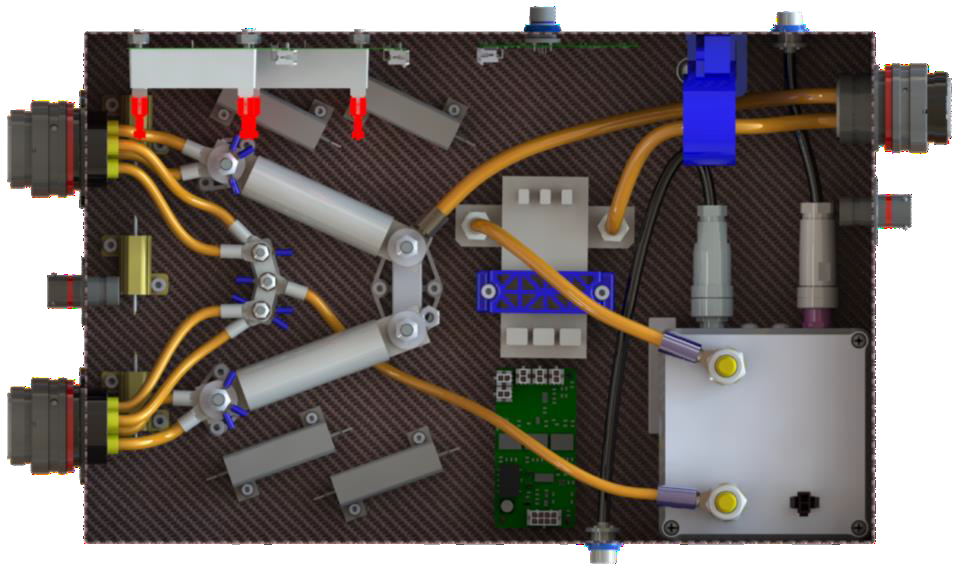
\includegraphics[width=7cm]
                            { img/2_formula_student/ddb.png }
                        \caption{Data and distribution box. \emph{BCN eMotorsport}}             
                    \end{minipage} \hfil
                    \begin{minipage}[c]{7cm}
                        \centering
                        \captionsetup{justification=centering}
                        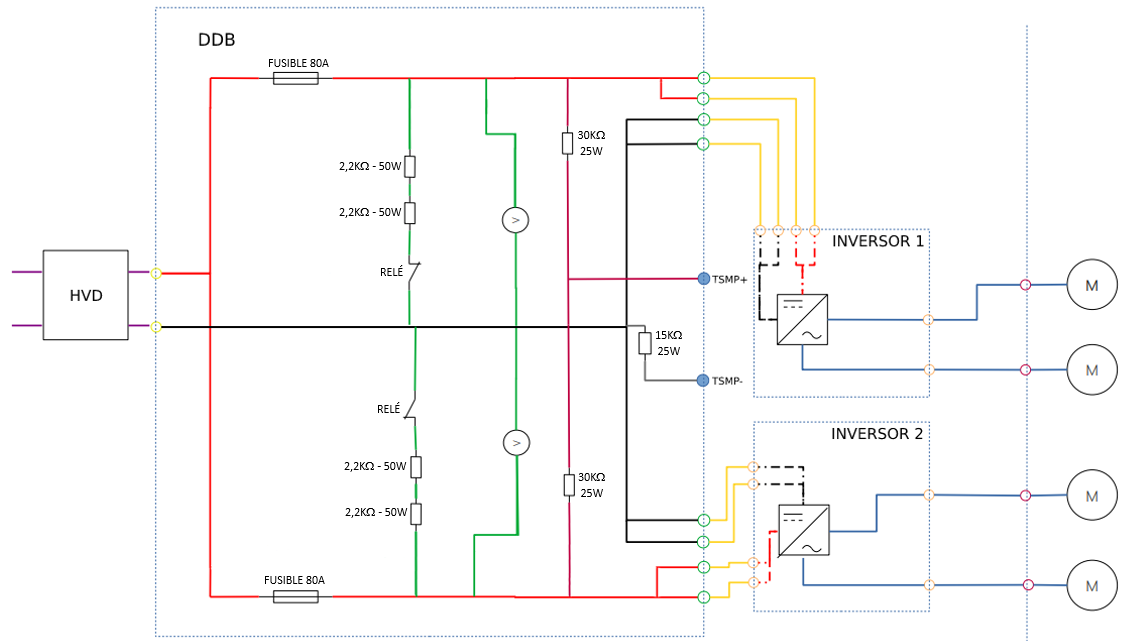
\includegraphics[width=7cm]
                            { img/2_formula_student/circuit.png }
                        \caption{Circuit de distribució. \emph{BCN eMotorsport}}                
                    \end{minipage} \hfil
                \end{figure}

            \item \textbf{Cablejat:}
                Pel cablejat del circuit d'alt voltatge es fa servir cablejat
                blindat Radox de la marca Huber\&Suhner. Per normativa, el
                cablejat ha de ser de color taronja \cite{fs_rules}.
        \end{itemize}
    }
}

\clearpage \section{Marc teòric del control motor}
Per desenvolupar l'algorisme de control es parteix dels models elèctrics del
motor i de l'inversor. El tipus de motor a utilitzar defineix certes topologies
per l'inversor, que a la seva vegada determina les estratègies de control a
emprar. La possibilitat de disposar de sensors de posició i velocitat, la
robustesa que es vol assolir i el compromís entre complexitat i rendiment també
determinen les estratègies del control.

L'algorisme de control a implementar és de camp orientat (\emph{Field Oriented
Control}) amb una estratègia de control MTPA (\emph{Maximum Torque per
Ampere}). Amb objectiu de permetre unes velocitats superiors, es fa ús del
debilitament de camp (\emph{Field Weakening}). El control de camp orientat
requereix una tècnica de modulació per convertir el vector de voltatge a la
sortida del controlador en una tensió mesurada en les fases de l'inversor. Per
aquesta funció es fa servir el \acs{SVPWM}. El diagrama de la figura
\ref{simple} ens dóna una idea de com es relacionen aquests elements.

\begin{figure}[!htb]
    \centering
    \captionsetup{justification=centering, margin=1cm}
    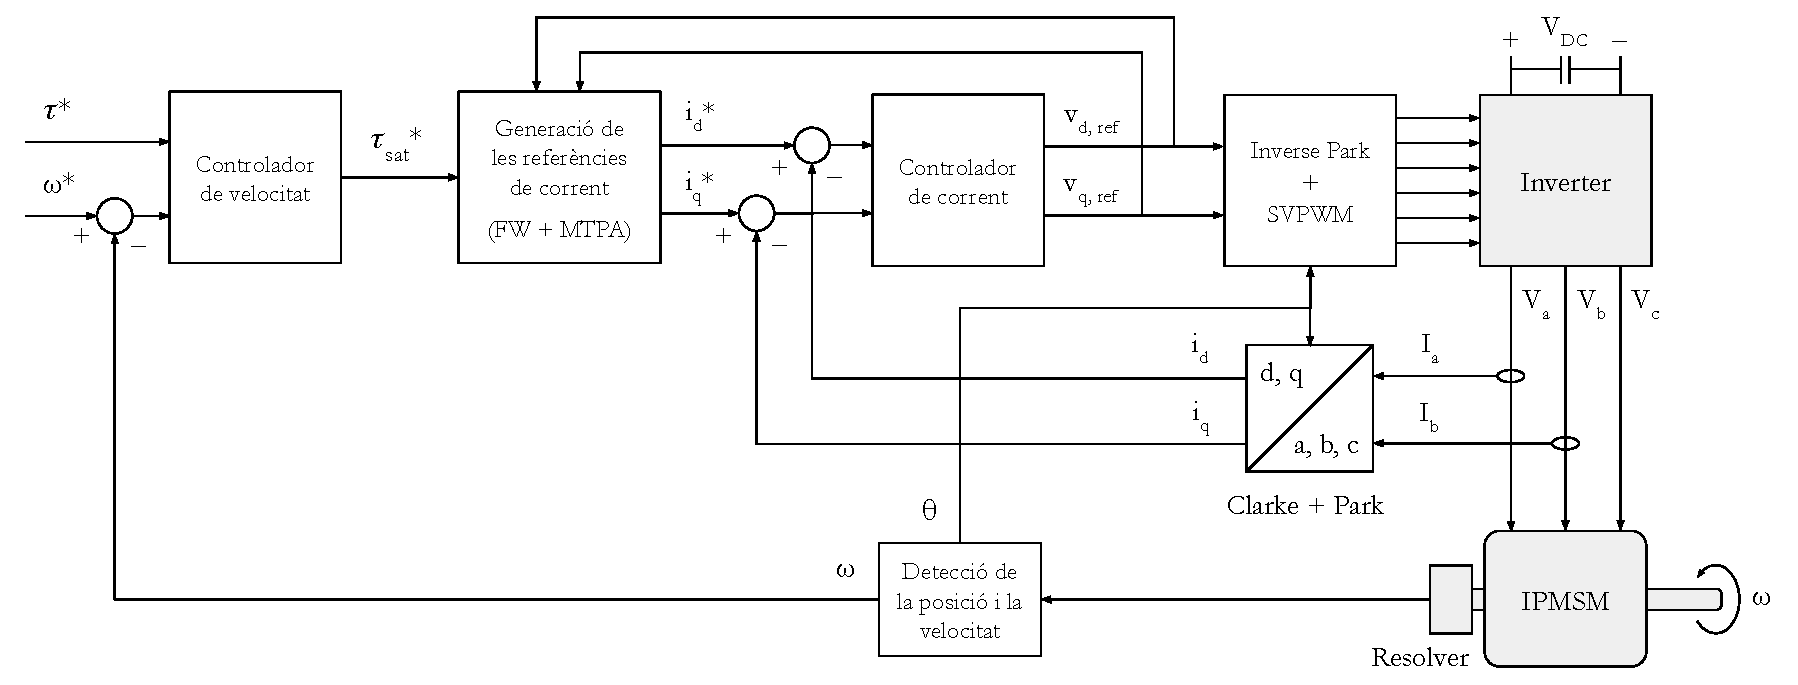
\includegraphics[width=14cm]
        { img/3_control_motor/simple.pdf }
    \caption[Diagrama de blocs del control]
        { Diagrama de blocs de l'algorisme control }
    \label{simple}
\end{figure}

\subsection{ Model elèctric del motor i de l'inversor }
{
    Un motor IPMSM es pot modelar a grans trets com una inductància i una
    resistència en serie per cada fase. En un motor trifàsic existeixen dos
    tipus de connexions, en estrella i en triangle. En el nostre cas, el
    connexionat és en estrella: les tres branques del motor s'uneixen en un
    punt intermig anomenat punt neutre i simbolitzat amb una $n$.

    L'equació de voltatges d'un motor síncron en el sistema de referència
    d-q\footnotemark per al nostre cas ve donada per l'equació 1:

    \footnotetext
    {   
        El sistema de referència d-q és un sistema de referència ortogonal
        bidimensional que es mou solidàriament amb el rotor. L'ús d'aquest
        sistema de referència linealitza alguns dels càlculs realitzats, que en
        cas contrari dependrien de la rotació del motor.
    }
    
    \begin{equation}
        \begin{bmatrix} v_d \\[5pt] v_q \end{bmatrix} =
        \begin{bmatrix}
            { R + \frac{d}{dt} L_d } & { -\omega L_q } \\[5pt]
            { \omega L_d } & { R + \frac{d}{dt} L_d }
        \end{bmatrix}
        \cdot \begin{bmatrix} i_q \\[5pt] i_d \end{bmatrix}
        + \begin{bmatrix} 0 \\[5pt] \omega \lambda_{pm} \end{bmatrix}
    \end{equation}

    on,
    \begin{description}
    {
        \item $\lambda_{pm}$ és el flux induït pels imats permanents al llarg de
        l'eix d-q
        \item $i_d, i_q$ són les components $d$ i $q$ del corrent induït
        \item $v_d, v_q$ són les components $d$ i $q$ del voltatge induït
        \item $L_d, L_q$ és la inductància del bobinat respecte als eixos $d$ i
        $q$
        \item $R$ és la resistència del bobinat
        \item $\omega$ és la velocitat angular del rotor
    }
    \end{description}

    \begin{figure}[!htb]
        \centering
        \captionsetup{justification=centering,margin=1.5cm}
        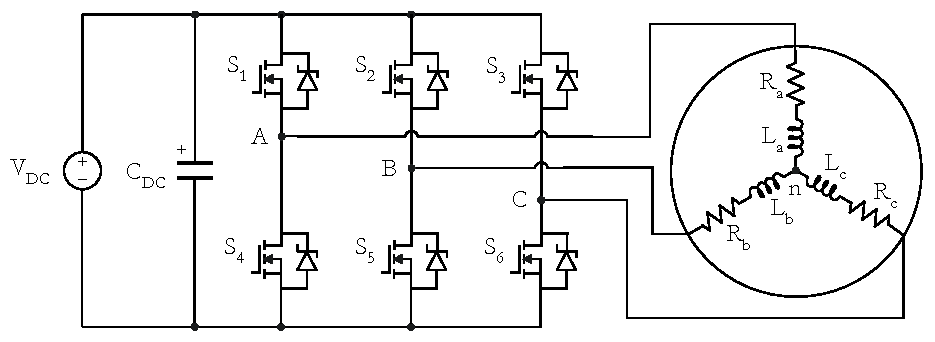
\includegraphics[width=12cm]
            { img/3_control_motor/inverter.pdf }
        \caption{ Circuit equivalent d'un inversor i motor trifàsics }
    \end{figure}

    Per conduir un motor trifàsic, l'inversor també ha de ser trifàsic. Cada
    una de les tres branques consta de dos transistors, formant el que
    es coneix com \emph{Half-Bridge}.
    
    La topologia emprada és la de dos nivells (\emph{Two Level Inverter, TLI}).
    L'elecció de la tipologia està justificada per membres anteriors de
    l'equip. A grans trets es pot dir que la decisió es basa en els següents
    factors:
    
    \begin{itemize}
        \item \textbf{Experiència:}
            L'equip disposa d'una experiència més amplia treballant amb
            inversors de dos nivells amb modulació per \ac{SVPWM}, ja que
            l'inversor Lenze actual presenta aquesta tipologia.

        \item \textbf{Bateria:}
            En cas d'implementar un inversor multinivell (MLI) la bateria
            hauria de dividir-se en dos, suposant un treball addicional per
            l'equip.

        \item \textbf{Estudi de pèrdues:}
            En l'estudi realitzat per l'equip, l'inversor TLI amb MOSFETs SiC i
            control per SVPWM va tenir les menors pèrdues per commutaci,
            aconseguint un aprofitament del bus DC del 90,7\% (no obstant, a
            costa d'una pitjor qualitat d'ona en termes de distorsió harmònica
            total, \acs{THD}).

        \item \textbf{Dimensions, pes i cost:}
            L'ús d'un inversor multinivell eleva el cost de l'inversor i el fa
            més voluminós i pesat en fer servir una major quantitat de
            transistors.

    \end{itemize}
}

\subsection{ Control de camp orientat }
{
    El control de camp orientat (\emph{Field Oriented Control}, FOC) és una de
    les tècniques de control més utilitzades quan es treballa amb motors
    d'imants permanents i motors d'inducció. Consisteix a controlar el corrent
    del motor una vegada sofert una sèrie de transformades (Park i Clarke) que
    sincronitzen els corrents amb el gir del rotor. En sincronitzar els
    corrents es poden aplicar tècniques de control lineal com els controladors
    proporcional-intregral (PI).

    \subsubsection{ Transformada de Clarke }
    {
        En un primer lloc, les mesures de corrent de les tres fases del motor
        (fases a, b i c) s'han de convertir a un sistema de referència de dos
        fases, formant l'espai estacionari $\alpha$-$\beta$. Per realitzar
        aquesta conversió s'empra la transformada de Clarke (o transformada
        $\alpha$-$\beta$ per la nomenclatura de les seves variables).
        L'expressió de la transformada de Clarke és la següent:

        \begin{equation}
            \begin{bmatrix} \alpha \\[5pt] \beta \\[5pt] \gamma \end{bmatrix} =
            \begin{bmatrix}
                \frac{2}{3} & -\frac{1}{3} & -\frac{1}{3} \\[5pt]
                0 & \frac{1}{\sqrt{3}} & -\frac{1}{\sqrt{3}} \\[5pt]
                \frac{1}{3} & \frac{1}{3} & \frac{1}{3}
            \end{bmatrix}
            \cdot \begin{bmatrix} a \\[5pt] b \\[5pt] c\end{bmatrix}
        \end{equation}

        La transformada de Clarke actua de manera que tots els punts situats
        sobre la semirrecta que surt de l'origen i creix paral·lela al vector
        de la fase $a$. De la mateixa manera, els punts situats sobre la
        semirrecta paral·lela a la fase $b$ passen a caure a sobre la
        semirrecta a 90º de la fase $a$.

        Com que el sistema trifàsic es de corrents balancejats, tenim que $i_a
        + i_b + i_c = 0$. Amb això, una de les tres branques de l'inversor
        (generalment el corrent anotat com $i_c$) es torna supèrflua, poguent
        simplificar així el càlcul de la transformada de Clarke. D'aquesta
        manera, l'equació implementada en el nostre cas pren la següent forma:

        \begin{equation}
            \begin{bmatrix} \alpha \\[5pt] \beta \end{bmatrix}
            = \frac{2}{3} \cdot
            \begin{bmatrix}
                1 & 0 \\[5pt]
                \frac{1}{\sqrt{3}} & \frac{1}{\sqrt{3}}
            \end{bmatrix}
            \cdot \begin{bmatrix} a \\[5pt] b \end{bmatrix}
        \end{equation}
    }

    \subsubsection{ Transformada de Park }
    {
        La següent transformació consisteix a cambiar el sistema de referència
        que té com vectors unitaris el vector paral·lel a l'eix del motor
        (conegut per vector directriu, annotat com $d$) i el vector perpendicular a
        aquest (conegut com vector de quadratura, annotat com $q$). En paraules
        llanes, es podria dir que ens muntem a sobre de l'eix del motor i
        començem a girar-hi solidàriament. És en aquest punt que la dependència
        amb l'angle desapareix i el valor de corrent resultant captura
        l'envolvent del senyal sinusoidal original. La transformació que
        s'empra per l'esmentat canvi és la transformada de Park, l'equació de
        la qual, en forma matricial, és:

        \begin{equation}
            \begin{bmatrix} q \\[5pt] d\\[5pt] 0 \end{bmatrix} = 
            \begin{bmatrix}
                cos(\theta) & sin(\theta) & 0 \\[5pt]
                -sin(\theta) & cos(\theta) & 0 \\[5pt]
                0 & 0 & 1
            \end{bmatrix}
            \cdot \begin{bmatrix} \alpha \\[5pt] \beta \\[5pt] \gamma \end{bmatrix}
        \end{equation}

        Veiem que per aplicar aquesta transformada necessitem el valor de
        l'angle del rotor. Aquest angle pot ser mesurat directament per mitjà
        d'un resolver o un encodificador, o d'altra banda es pot estimar a
        partir de les mesures de corrent fent servir observadors.
    }

    \subsubsection{ Transformada inversa de Park }
    {
        Un cop realitzat el control del corrent en el marc de referència d-q,
        la tensió obtinguda s'ha de transformar al marc de referència en el que
        opera el SVPWM, que es el d'$\alpha$-$\beta$. Per aquesta raó s'aplica
        la transformada inversa de Park, que s'obtè invertint la matriu de
        rotació de la transformada de Park:

        \begin{equation}
            \begin{bmatrix} \alpha \\[5pt] \beta \end{bmatrix} = 
            \begin{bmatrix}
                cos(\theta) & sin(\theta) \\[5pt]
                sin(\theta) & -cos(\theta) \\[5pt]
            \end{bmatrix}
            \cdot \begin{bmatrix} q \\[5pt] d \end{bmatrix} 
        \end{equation}
    }
}

\subsection{ Maximum Torque per Ampere }
{
    L'equació \ac{MTPA} ens permet obtenir el màxim parell donat un corrent
    determinat. L'equació es dedueix a partir del parell electromagnètic d'un
    motor PMSM, que pot ser expressat com:
    
    \begin{equation}
        \tau_{em} = \frac{3}{2}p(\lambda_{pm} i_q + (L_d - L_q) i_d i_q)
    \end{equation}

    on,
    \begin{description}
    {
        \item $\tau_{em}$ és el parell electromagnètic
        \item $\lambda_{pm}$ és el flux induït pels imats permanents al llarg
        de l'eix d-q
        \item $i_d, i_q$ són les components $d$ i $q$ del corrent induït
        \item $v_d, v_q$ són les components $d$ i $q$ del voltatge induït
        \item $L_d, L_q$ és la inductància del bobinat respecte als eixos $d$ i
        $q$
        \item $R$ és la resistència del bobinat
        \item $\omega$ és la velocitat angular del rotor
    }
    \end{description}

    Per obtenir un parell màxim, s'han de complir la següent condició
    d'optimització:
    
    \begin{equation}
        \left\{
            \begin{aligned}
                \frac{\partial (\tau_{em} / i_s)}{\partial i_d} = 0 \\
                \frac{\partial (\tau_{em} / i_s)}{\partial i_q} = 0
            \end{aligned}
        \right.
    \end{equation}

    Així, aplicant les condicions a l'equació de torque obtenim el corrent
    $i_d$ a injectar a partir del corrent $i_q$:

    \begin{equation}
        i_d = \frac{-\lambda_m + \sqrt{\lambda_m^2 + 4 (L_d - L_q)^2 i_q^2}}{ 2 (L_d - L_q) }
    \end{equation}

    % \begin{figure}[!htb]
    %     \centering
    %     \captionsetup{justification=centering, margin=1.5cm}
    %     \includegraphics[width=13cm]
    %         { img/3_control_motor/mtpa_fw.pdf }
    %     \caption[Regió de debilitament de camp]
    %         { Regió de debilitament de camp }
    %     \begin{quote}
    %         La regió en la que es produeix el debilitament de camp es troba
    %         limitada per les corves de \ac{MTPA} i \ac{MTPV}, així com les
    %         corves de corrent i voltatge màxims. 
    %     \end{quote}
    % \end{figure}
}

\subsection{ Debilitament de camp }
{
    El debilitament de camp o debilitament de flux (en anglés, \emph{Field
    Weakening}) és una tècnica per augmentar la velocitat d'un motor elèctric
    per damunt de la seva capacitat nominal, a càrreg de reduir el par motor.
    S'aplica en els casos en què es requereix obtenir una major velocitat i és
    admisible disposar de menor par motor. És molt utilitzada en motors
    d'imants pemanents, ja que es troben limitats en velocitat quan la tensió
    de l'estàtor assoleix el límit de sortida de l'inversor.

    El debilitament de camp fa ús dels corrents $i_q$i $q_d$ de l'inversor per
    contrarrestar el flux magnètic de l'entreferro que generen els imants del
    rotor. En específic, el control de debilitament de camp consisteix a reduir
    el flux de l'entreferro resultant associat als imants permanents,
    $\lambda_{pm}$, injectant un corrent $i_d$ negatiu.

    El debilitament de camp es pot implementar trobant la relació entre els
    corrents i la velocitat en aquest mode de funcionament, o bé tancant un
    llaç de control amb un controlador PI en el que la consigna sigui
    el valor de voltatge màxim del bus DC (multiplicat per un factor de
    seguretat) i la sortida el corrent $i_d$ necessari per mantenir el bus DC
    plenament utilitzat.
}

\subsection{ Modulació d'amplada de pulsos }
{ 
    Existeixen diverses tècniques de modulació d'amplada de pulsos. L'objectiu
    de la modulació d'amplada de pulsos és accionar els transistors de
    l'inversor per sintetitzar la tensió desitjada a cada una de les branques.

    Per a l'inversor de dos nivells les tècniques de modulació es reduixen a
    la pràctica a la modulació per mitjà de senyal sinusoidal o SPWM
    (\emph{Sinusoidal Pulse Width Modulation}) i a la modulació per mitjà de
    vectors espacials o SVPWM (\emph{Space Vectoring Pulse Width Modulation}).

    \subsubsection{ SPWM } 
    { 
        La modulació senoidal d'amplada de pulsos (\emph{Sinusoidal Pulse Width
        Modulation, SPWM}) és una tècnica de generació de PWM consistent a
        comparar el senyal de voltatge AC de referència amb un senyal portador
        triangular de freqüència igual a la freqüència de conmutació dels
        interruptors. Se sol utilitzar per la seva simplicitat a l'hora
        d'implementar-lo. Quan el senyal de referència es major que el senyal
        triangular, l'interruptor ``high" de la fase s'activa; en cas contrari,
        s'activa l'interruptor ``low".

        \begin{figure}[!htb]
            \centering
            \captionsetup{justification=centering, margin=1.5cm}
            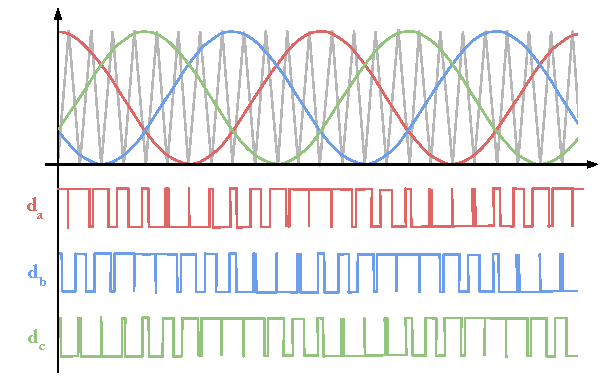
\includegraphics[width=7cm]
                { img/3_control_motor/spwm.pdf }
            \caption{ Generació dels cicles de treball en el SPWM.}
        \end{figure}
    }

    \begin{figure}[!htb]
        \centering
        \captionsetup{justification=centering,margin=1.5cm}
        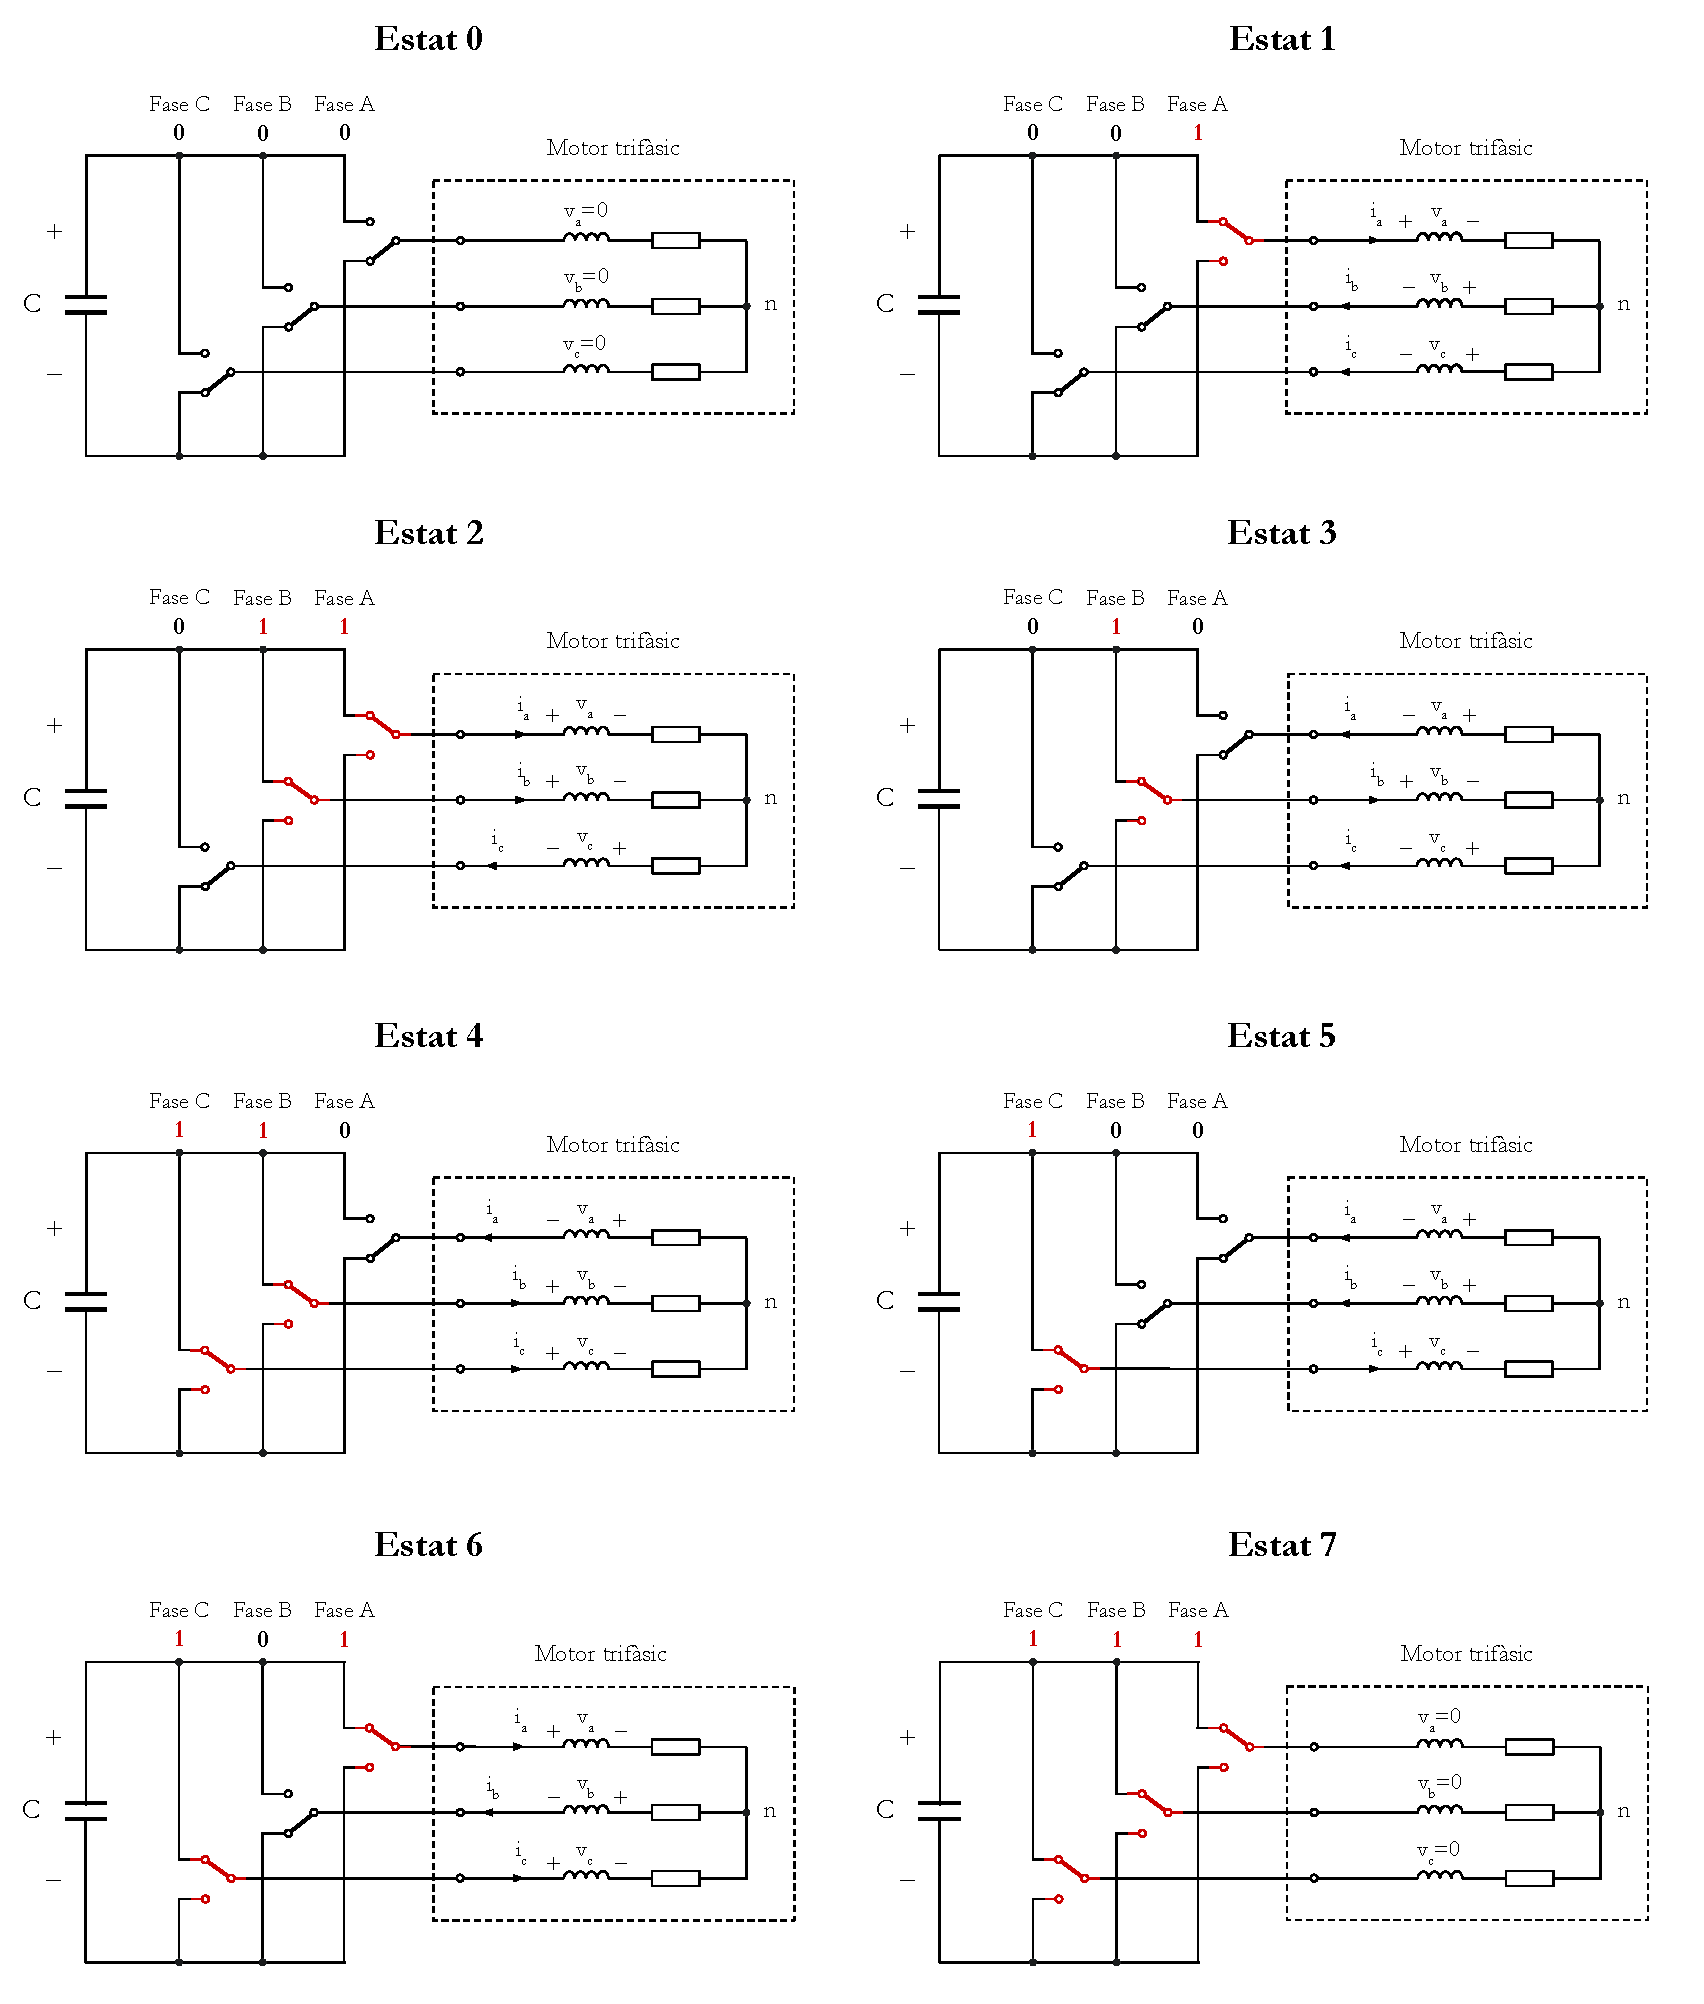
\includegraphics[width=14.5cm]
            { img/3_control_motor/states_inverter.pdf }
        \caption[Estats de l'inversor]
            { Estats de l'inversor}
        \label{estats}
    \end{figure}

    \newpage
    \subsubsection{ SVPWM } 
    { 
        La modulació d'amplada de pulsos per vectors espacials (SVPWM) empra la
        representació vectorial de un sistema polifàsic per generar el PWM. A
        gran trets l'objectiu es descomposar el vector de voltatge de
        referència en vectors associats a cada un dels estats de commutació
        d'un inversor. L'ús de la modulació SVPWM permet aprofitar el bus
        DC molt més que amb la modulació sinusoinal SPWM més tradicional, d'un
        90,7\% contra un 78,5\%.

        En un inversor trifàsic, cada branca compta amb un parell de
        transistors que treballen conjuntament com un commutador (i evitant el
        curtcircuit del bus DC). En tot moment els bobinats de cada branca del
        motor estan connectats al pol positiu o el negatiu del bus DC. Com que
        tenim a la nostra disposició 3 parells de transistors i dos estats
        posibles per branca, es configuren 8 estats, dos d'ells nuls (estats 0
        i 7), ja que no hi ha caiguda de tensió en cap dels bobinats del motor.
        La configuració dels possibles estats es pot veure en la figura
        \ref{estats}.

        Podem associar cada un d'aquests estats a un vector en l'espai de
        referència $\alpha\-\beta$, de manera que configuren un hexàgon,
        caracterísitc del SVPWM, tal i com es representa en la figura
        \ref{hexagon}. Així, es generen 6 sectors diferents delimitats pels
        vectors dels estats 1 a 6. Els estats 0 i 7, per la seva banda, queden
        en el centre del sistema de referència.

        \begin{figure}[!htb]
            \centering
            \captionsetup{justification=centering,margin=1.5cm}
            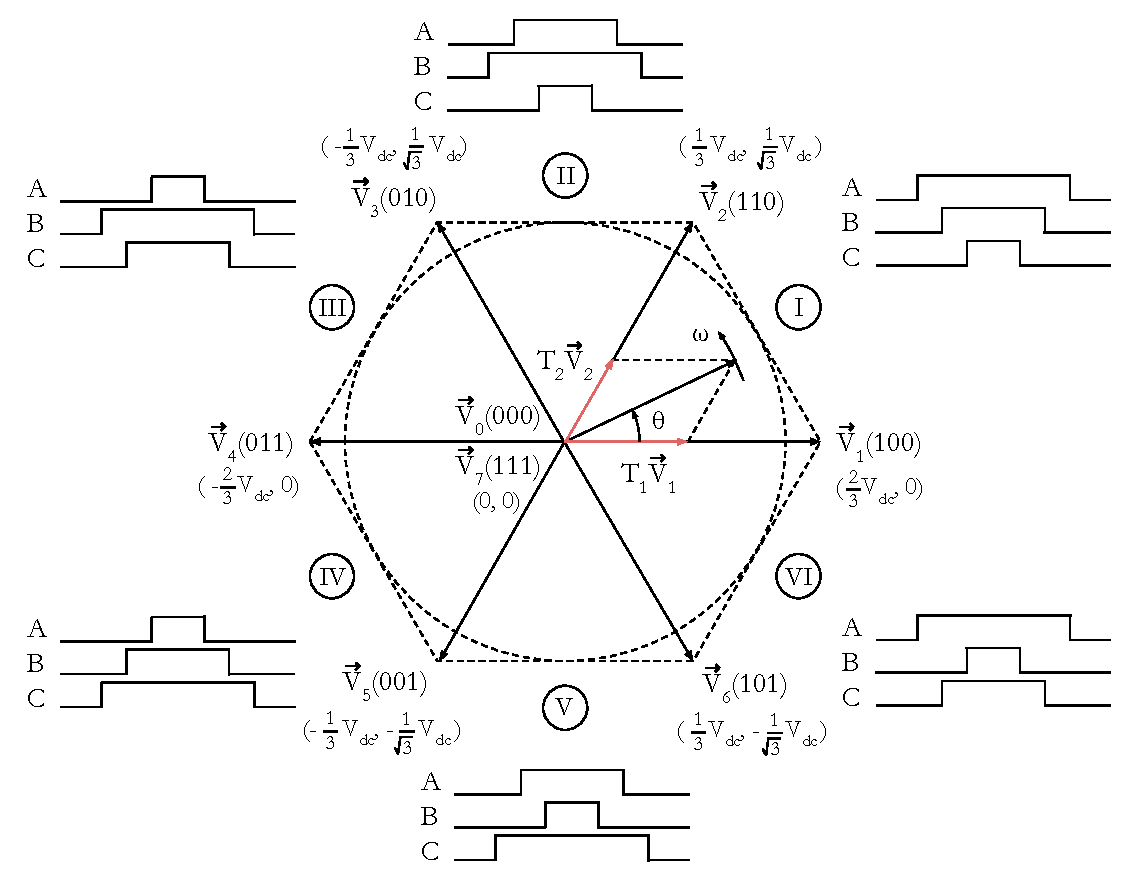
\includegraphics[width=15cm]
                { img/3_control_motor/SVPWM.pdf }
            \caption[Síntesi del vector espacial]
                { Síntesi del vector espacial. \textit{Elaboració pròpia.} }
                \label{hexagon}
        \end{figure}

        Si representem el vector de voltatge de referència en aquest marc,
        podem veure que cau entre dos estats de conmutació. Per tant, podem
        sintetitzar-lo com la suma dels vectors escalats de les commutacions
        més properes, més una contribució del vector nul 0 o 7. L'escalat dels
        vectors és directament proporcional al temps en què l'inversor es troba
        en aquell estat amb respecte el periode de commutació escollit.

        L'algorisme de SVPWM implementat es basa en la identificació del sector
        per calcular el cicles de treball que s'han de comparar amb el senyal
        triangular. El sector s'identifica inspeccionant que les components del
        vector de referència es trobin per damunt o per baix de les tres rectes
        que formen els vectors dels estats de commutació: $v_b - \sqrt{3} > 0$,
        $v_b < 0$ i $v_b + \sqrt{3} > 0$. Això genera una codificació en binari
        corresponent als nombres entre el 1 i el 6, que s'han de mapejar als
        sectors I-VI: $2 \rightarrow I,\ 6 \rightarrow II,\ 4 \rightarrow III,\
        5 \rightarrow IV,\ 1 \rightarrow V\ i\ 3 \rightarrow VI$.

        A continuació, es calculen els cicles de treball pel generador de PWM.
        Aïllant el primer dels sectors (I) en la figura \ref{hexagon}, es pot
        treure geomètricament una relació entre el vector de referència i el
        temps d'encesa de cada estat:

        \begin{equation}
            t_1 = \frac{T_s}{V_{dc}} (\frac{3}{2} V_\alpha-\frac{\sqrt{3}}{2} V_\beta);\ \ \ \ \ 
            t_2 = \sqrt{3} \frac{T_s}{V_{dc}} V_\beta;\ \ \ \ \ 
            t_0 = T_s - t_1 - t_2
        \end{equation}

        Aquest càlcul es pot aplicar de manera simètrica per la resta dels
        sectors, tenint en compte la seva posició amb respecte els eixos del
        sistema de referència $\alpha\-\beta$. Definint les variables X, Y i Z,
        i identificant el sector on ens trobem, podem calcular de manera global
        els temps $t_1$, $t_2$ i $t_0$. Si, a més, considerem que en el sectors
        impars els temps $t_1$ i $t_2$ estan intercanviats respecte els vectors
        pars, es defineixen uns temps $t_1'$ i $t_2'$ en funció de X, Y i Z,
        que es recullen en la taula de sota.

        \begin{equation}
            X = \frac{\sqrt{3}}{2}\frac{\sqrt{3}}{V_{DC}}v_\alpha;\ \ \ \ \ \
            Y = \frac{1}{2}\frac{\sqrt{3}}{V_{DC}}v_\beta;\ \ \ \ \ \
            Z = \frac{\sqrt{3}}{V_{DC}}v_\beta
        \end{equation}

        \begin{table}[!htb]
            \caption{Càlcul dels temps d'encesa}
            \centering
            
            \begin{tabular}{c r r r r r r}
                \toprule
                    {Sector} & I & II & III & IV & V & VI \\
                \midrule
                    $t_1'$ & Z & Y & X & -Z & -Y & -X \\
                    $t_1'$ & X & -Z & -Y & -X & Z & Y \\ 
                \bottomrule
            \end{tabular}
        \end{table}

        Finalment, per obtenir un temps d'encesa per cada fase agrupem els
        temps $t_1'$, $t_2'$ i $t_0$ segons el diagrama de la figura
        \ref{encesa}. La seqüència de commutació comença amb $t_0$, continua
        amb $t_1'$, segueix amb $t_2'$ i just abans d'arribar a mig periode,
        torna a $t_0$. Com que el senyal triangular és centrat, el PWM també ho
        és i per simetria la seqüència es repiteix en sentit contrari fins
        sumar un periode de commutació. Com que hi han dues aparacions de $t_1'$
        i de $t_2'$, el seu valor es divideix per la meitat; mentres que $t_0$
        es divideix entre quatre en aparèixer quatre vegades, de tal manera que
        se segueix complint $t_1' + t_2' + t_0 = T_s$. Així, els valors de
        l'amplada de cada pols, $t_x$, $t_y$ i $t_z$, es calculen com:

        \begin{equation}
            t_x = \frac{1}{4}(1-t_1'-t_2');\ \ \ \ \ \
            t_y = \frac{1}{4}(1-t_1'+t_2');\ \ \ \ \ \
            t_z = \frac{1}{4}(1+t_1'+t_2')
        \end{equation}

        Per últim, cal assignar el valor de $t_x$, $t_y$ i $t_z$ a cada una de
        les fases del commutador, seguint el esquema de la taula següent:

        \begin{table}[!htb]
            \caption{Assignació dels temps calculats a cada fase de l'inversor}
            \centering
            
            \begin{tabular}{c r r r r r r}
                \toprule
                    {Fase} & I & II & III & IV & V & VI \\
                \midrule
                    A & $t_x$ & $t_y$ & $t_z$ & $t_z$ & $t_y$ & $t_x$ \\
                    B & $t_y$ & $t_x$ & $t_x$ & $t_y$ & $t_x$ & $t_x$ \\ 
                    C & $t_z$ & $t_z$ & $t_y$ & $t_x$ & $t_x$ & $t_y$ \\ 
                \bottomrule
            \end{tabular}
        \end{table}

        \begin{figure}[!htb]
            \centering
            \captionsetup{justification=centering}
            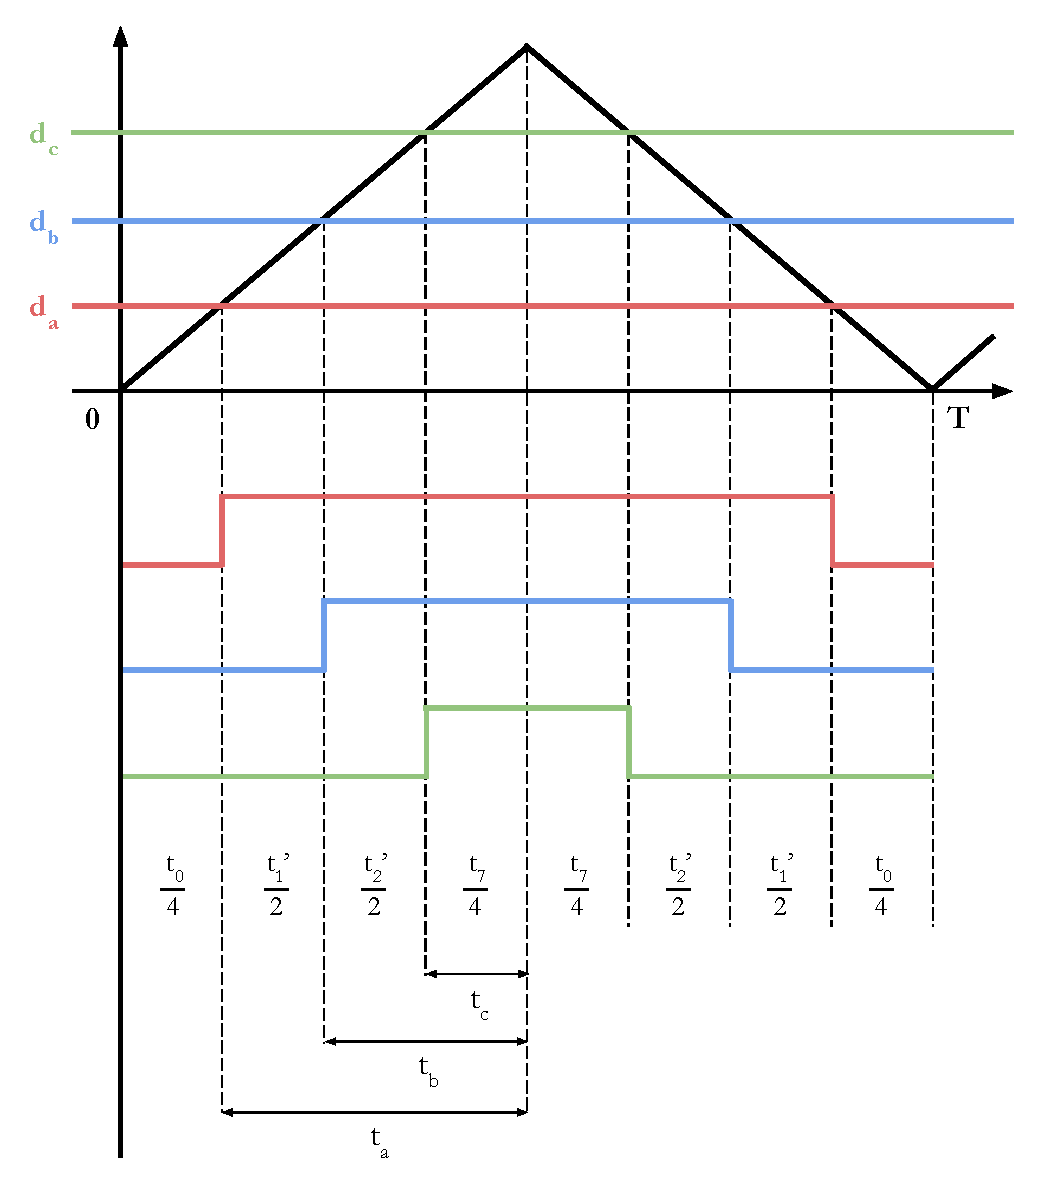
\includegraphics[width=9.5cm]
                { ../img/3_control_motor/encesa.pdf }
            \caption{ Càlcul del temps d'encesa }
            \label{encesa}   
        \end{figure}  

        \begin{figure}[!htb]
            \centering
            \captionsetup{justification=centering}
            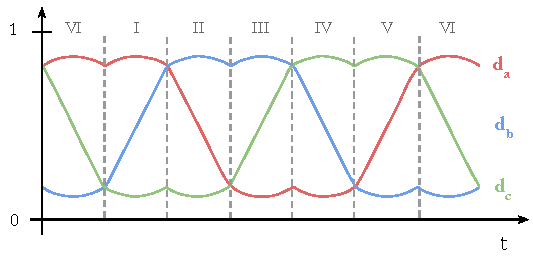
\includegraphics[width=10cm]
                { img/3_control_motor/duty.pdf }
            \caption[Cicles de treball obtinguts amb SVPWM]
                { 
                    Evolució del cicles de treball característica del SVPWM, a
                    mesura que el vector de referència passa pels diferents
                    sectors. 
                }          
        \end{figure}
    }

    \newpage
    \subsection{ Altres elements de l'algorisme de control }
    {
        L'algorisme de control necessita d'altres elements addicionals pel seu
        funcionament. 
        
        El primer d'aquests elements és la detecció de l'angle i la velocitat
        angular del rotor a partir de les mesures del resolver. Hi ha diverses
        maneres de realitzar aquesta detecció. Per aquest projecte
        s'ha decidir emprar un Resolver-to-Digital (\acs{R/D}), que es un circuit
        integrat específic per digitalitzar les mesures del resolver i que es
        basa en un sistema de control PLL. El model escollit és l'AD2S1210
        del fabricant \emph{Analog Devices} \cite{rtd}.
        
        En segon lloc hi trobem el controlador de velocitat angular. La seva
        funcionalitat principal és assegurar que la velocitat angular segueix a
        la consigna variant el valor del parell per mitjà d'una doble saturació.
    
        Per últim, s'han de considerar els elements de limitadors que
        proporcionen seguretat al control, de manera que les tensions i els
        corrents no superin els valors màxims imposats pel hardware. D'aquesta
        manera, trobem saturadors per saturar les referències de corrent $i_d*$
        i $i_q*$ i un limitador del mòdul de voltatge per saturar les
        referències de tensió $v_{d,ref}$ i $v_{q,ref}$.

        \begin{figure}[!htb]
            \centering
            \captionsetup{justification=centering, margin=1cm}
            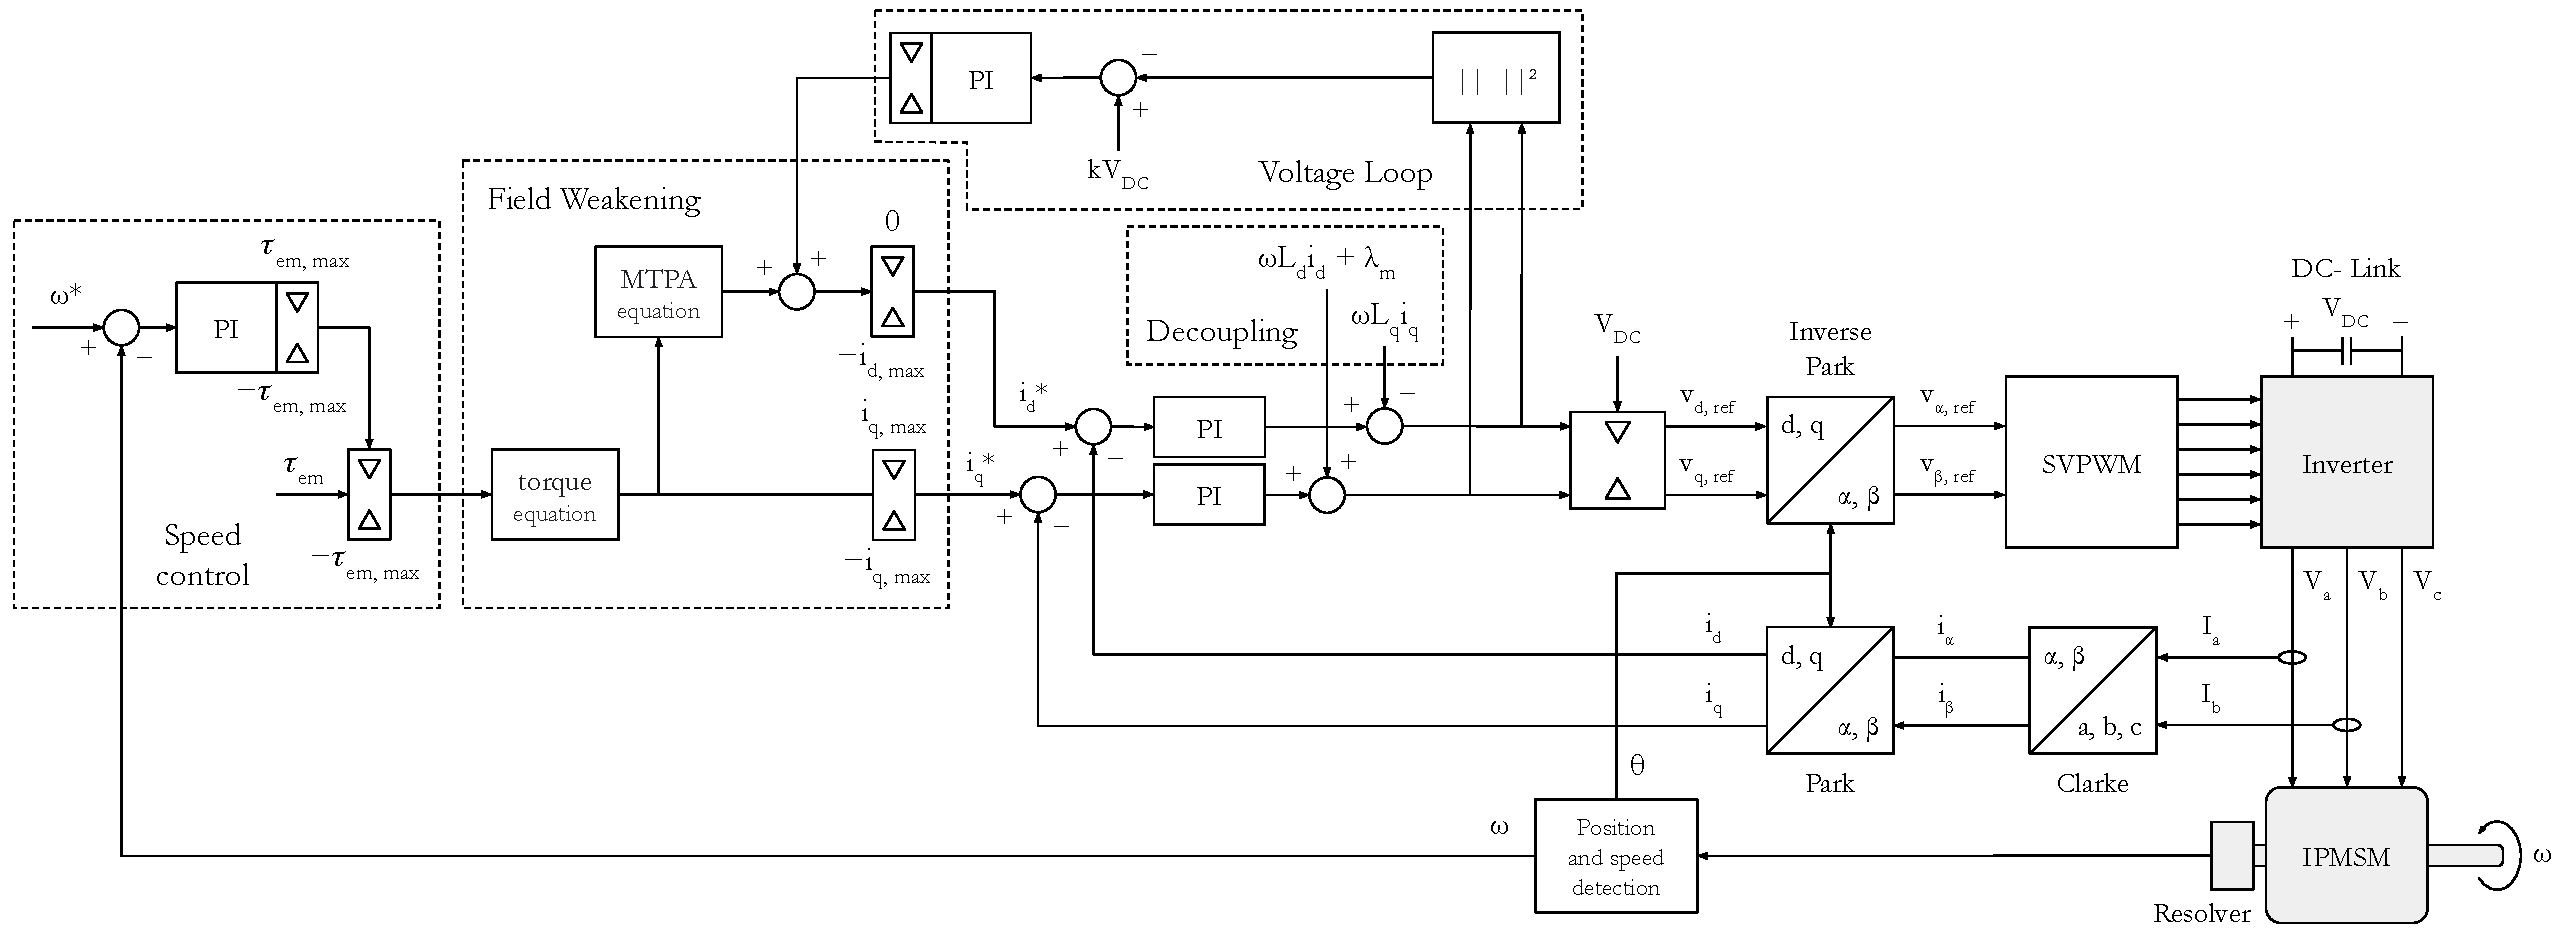
\includegraphics[width=15.75cm]
                { img/3_control_motor/control.pdf }
            \caption[Diagrama de blocs del control]
                { Diagrama de blocs complet de l'algorisme control }
            \label{diagrama}
        \end{figure}
    }
}

\clearpage \section{Disseny i implementació}
En aquest capítol s'exposaran les decisions presses a nivell de disseny, tant
d'arquitectura com hardware escollit i programació de la capa de seguretat. Es
continuarà amb l'anàlisi dels components de lògica prograble i d'arquitectura
de codi desenvolupat.

\subsection{ Proposta de disseny }
{
    Per a la implementació del control s'ha decidit utilitzar una arquitectura
    dual basada en lògica programable i en microprocessador. La decisió
    d'implementar el control en lògica programable en comptes d'utilitzar una
    arquitectura basada únicament en microprocessador o FPGA es justifica
    principalment per tres motius.

    En primer lloc, treballar amb una placa d'evaluació que incorpori aquesta
    arquitectura ens permet tenir més flexibilitat quan al disseny, poguent
    decidir si implementar un nou component en software o hardware segons
    evolucioni el projecte. Aquesta major flexibilitat de disseny és força
    interessant en el projecte de l'inversor, ja que permet, per exemple, la
    millora constant de l'algorisme de control per part de futurs membres.

    En segon lloc, la FPGA permet disposar de paral·lelisme real i
    temporització precisa, característiques que es tornen molt atractives en
    augmentar la freqüència de conmutació de l'inversor, sobretot fent servir
    MOSFETs SiC que poden treballar a altes freqüències. Actualment l'inversor
    està dissenyat per conmutar a 16 kHz, però la implementació en FPGA permet
    arribar a freqüències superiors que serien difícils d'assolir implementant
    l'algorisme de control en microcontrolador o microprocessador. De fet, amb
    FPGA es pot arribar inclús a aplicar un control en temps real.

    Finalment, en últim lloc, l'arquitectura de processador permet un
    desenvolupament més ràpid de les parts que no necessiten la velocitat i
    paral·leldismee la FPGA, ja que la descripció de lògica en hardware és més
    vulnerable a errades de programació i les eines de depuració i simulació no
    son tan potents com en software. Per aquesta raó es programa en software la
    interfície d'usuari, la comunicació amb la resta del vehicle i el
    monitoreig de sensors.

    No obstant, s'ha de tenir en compte que l'arquitectura dual també presenta
    inconvenients. La major contrapartida prové de la dificultat de la
    programació de la FPGA i la gestió de la comunicació entre la FPGA i el
    microprocessador. Això es degut principalment a la complexitat i opacitat
    en quan a documentació de les eines de desenvolupament en FPGA com és
    Vivado. Aquestes eines són majoritàriament propietàries i tancades; per
    tant, depenen de la dodumentació lliurada pel fabricant. En conseqüència,
    es prevenen dificultats en la transmissió del coneixement. És per això que
    s'ha posat especial interès als fluxos de treball i l'arquitectura de la
    FPGA, sent aquest un front no totalment resolert en el moment de
    l'escriptura la memòria.

    Seguint aquests motius es decideix utilitzar un SoC que incorpori aquesta
    arquitectura dual. L'avantatge respecte a un SoM és que en estar tots els
    dispositius (FPGA, microprocessadors, memòria i inclús ADCs) en un mateix
    xip la velocitat de comunicació entre aquests és molt reduida, permetent
    una operació a freqüències més altes. Addicionalment, es millora el consum
    energètic en ser dispositius més petits associats al mateix xip.

    No obstant això, l'equip no compta amb els coneixements ni els recursos per
    realitzar una placa d'acondicionament i adaptació d'un SoC. Per aquesta
    raó, es va decantar per utilitzar una placa de desenvolupament comercial.
}

\subsection{ Placa de desenvolupament }
{ 
    A l'inici del projecte, l'equip disposava d'una placa de desenvolupament
    Diligent Cora Z7-10, basada en el \ac{SoC} Zynq-7010 de Xilinx. Amb aquesta
    placa es va arribar a realitzar el testeig dels senyals dels Gate Drivers
    montats en placa \cite{coraz7} \cite{mikel}.

    \begin{figure}[!htb]
        \centering
        \begin{minipage}[c]{8cm}
            \centering
            \captionsetup{justification=centering}
            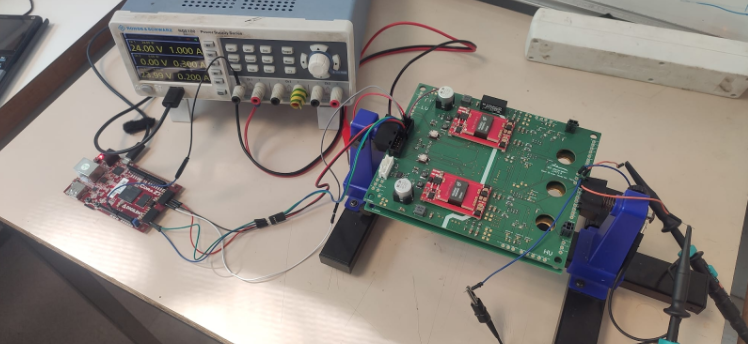
\includegraphics[width=8cm]
                { img/4_implementacio/cora_mikel.png }
            \caption{ La Cora Z-7 en la prova dels Gate Drivers. \emph{BCN eMotorsport.} }                
        \end{minipage} \hfil
        \begin{minipage}[c]{7.5cm}
            \centering
            \captionsetup{justification=centering}
            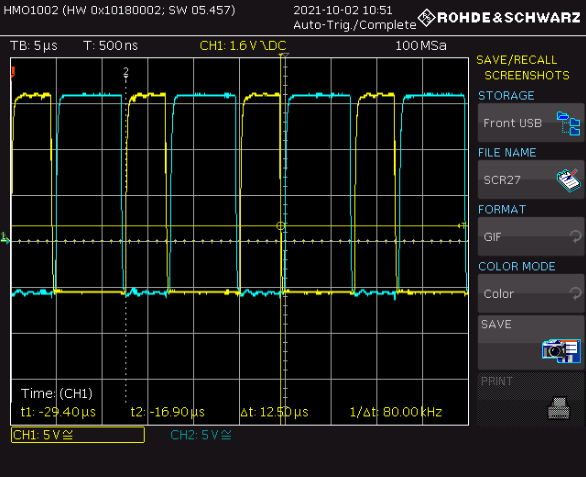
\includegraphics[width=5.5cm]
                { img/4_implementacio/gate_drivers.png }
            \caption{ Captura de l'oscil·loscopi. \emph{BCN eMotorsport.} }                
        \end{minipage} \hfil
    \end{figure} 

    De cara a una implementació futura de l'inversor, es va decidir substituir
    la Cora Z7-10 per una placa que facilités el desenvolupament de l'inversor
    i que millorés la implementació final de l'inversor de cara a l'any vinent.
    Es volia trobar una placa amb més recursos lògics i un major nombre
    d'entrades de propòsit general (GPIO) per poder implementar el control pels
    quatre motors en la mateixa placa. També es va procurar que la
    documentació fos bona i extensa.

    El primer que es va pensar es si continuar amb el mateix fabricant del SoC,
    Xilinx. Després d'un anàlisi de la competència, es va veure que Xilinx
    continuava sent la millor opció: 
    
    \begin{itemize}
        \item
            Es tracta del major fabricant de FPGAs en l'actualitat, amb una
            quota de mercat per facturació superior al 50\%, desbancant als
            seus competidors com són Altera d'Intel o Lattice. En conseqüència,
            la comunitat al voltant els seus productes és més extensa i és més
            senzill trobar recursos de consulta.
        \item 
            L'equip ja disposava d'un \emph{know-how} de l'ús de les eines de
            desenvolupament de Xilinx, en específic de la suite
            Vitis/Vivado\textsuperscript{\textregistered}. Es tracten d'eines
            bastant complexes i intimidants en un principi, però resulten ser
            potents en quan a funcionalitat.
    \end{itemize}

    Finalment es va decidir comprar la Z-Turn del fabricant Make Your Idea
    Real, que era una de les poques plaques disponibles degut a l'actual falta
    de stock de components electrònics, en especial semiconductors. Compleix
    les especifiacions demanades a un preu competitiu. Com que la família de
    SoC es la mateixa, gran part del \emph{know-how} del equip és aplicable a
    la nova placa \cite{zturn}.

    \begin{figure}[!htb]
        \centering
        \begin{minipage}[c]{7cm}
            \centering
            \captionsetup{justification=centering}
            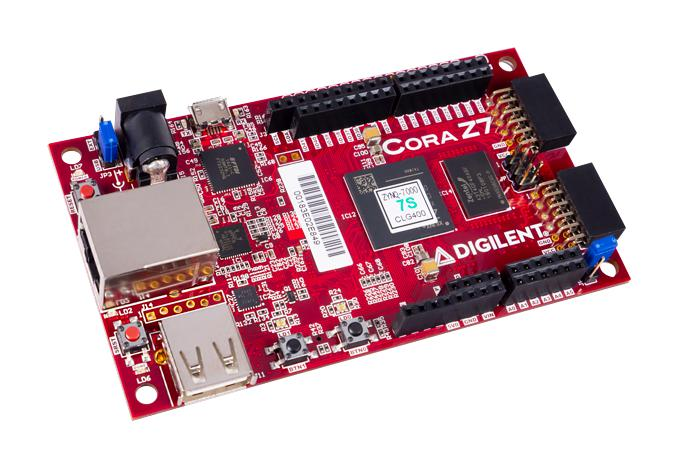
\includegraphics[width=7cm]
                { img/4_implementacio/cora-z7.jpg }
            \caption{ Digilent Cora Z7-10 }                
        \end{minipage} \hfil
        \begin{minipage}[c]{7cm}
            \centering
            \captionsetup{justification=centering}
            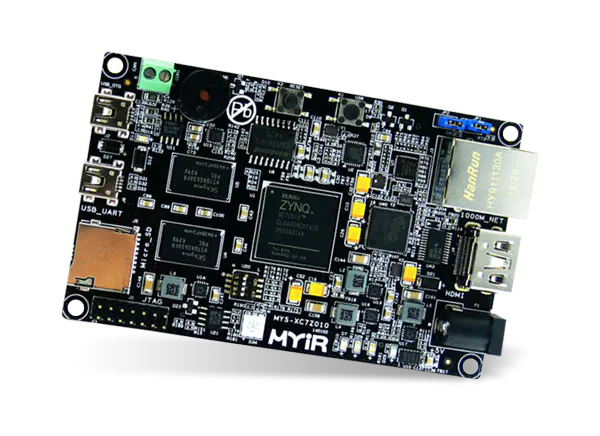
\includegraphics[width=6.5cm]
                { img/4_implementacio/zturn.png }
            \caption{ MIYR Z-Turn }                
        \end{minipage} \hfil
    \end{figure} 

    \begin{table}[!htb]
        \caption{ Comparativa entre la Digilent Cora Z7-10 i la MYIR Z-Turn }
        \centering
        \tablefirsthead{}
        \tablehead{}
        \tabletail{}
        \tablelasttail{}
        \renewcommand{\arraystretch}{1.3}
    
        \begin{supertabular} {|l|l|m{4.5cm}|m{4.5cm}|}
            \hline
                \multicolumn{2}{|l|}{ \textbf{ SoM } } & 
                \textbf{ Digilent Cora Z7-10 } & 
                \textbf{ MYIR Z-Turn } \\
            \hhline{|=|=|=|=|} \multirow{10}{*}{ SoC } & 
                { Família } & \multicolumn{2}{|c|}{ Xilinx Zynq-7000 } \\
            \cline{2-4} &
                { Model } &
                    { Z-7010 XC7Z010 } & 
                    { Z-7020 XC7Z020 } \\
            \cline{2-4} &
                { Microprocessador } & 
                    \multicolumn{2}{|c|}{ ARM Cortex-A9 de 2 nuclis } \\
            \cline{2-4} & 
                { Slices } &
                    { 4.400 } & 
                    { 13.300 } \\
            \cline{2-4} & 
                { Blocs \acs{DSP} dedicats } &
                    { 80 } & 
                    { 220 } \\
            \cline{2-4} & 
                { Look-Up tables (LUTs) } &
                    { 17.600 } & 
                    { 53.200 } \\
            \cline{2-4} & 
                { Flip-flops } &
                    { 35.200 } & 
                    { 106.400 } \\
            \cline{2-4} & 
                { Block RAM } &
                    { 2.1 Mb (60 blocks) } & 
                    { 4.9 Mb (140 blcks) } \\
            \cline{2-4} & 
                { Freq. de rellotge màx. } & \multicolumn{2}{|c|}{ 667 MHz } \\
            \cline{2-4} & 
                { ADC } & \multicolumn{2}{|c|}{ 2x 12 bits ADC @ 1 MSPS } \\
            \hhline{|=|=|=|=|}
                \multicolumn{2}{|l|}{ Memory } &
                { 
                    \medskip     
                    512 MB DDR3 SDRAM \newline (16-bit bus) \newline
                    SD card slot
                } &
                { 
                    \medskip 
                    1 GB DDR3 SDRAM \newline (32-bit bus) \newline
                    SD card slot
                } \\            
            \hline            
                \multicolumn{2}{|l|}{ Connectors } &
                { 
                    \medskip 
                    61x user GPIO \newline
                    1x USB-UART \newline
                    1x JTAG for debbuging \newline
                    1x Ethernet \newline
                    2x Pmod connectors \newline
                    \newline
                } &
                {  
                    \medskip
                    106x user GPIO \newline
                    1x USB-UART \newline
                    1x JTAG for debbuging \newline
                    1x Ethernet \newline
                    1x CAN \newline
                    1x HDMI
                } \\
            \hline
                \multicolumn{2}{|l|}{ Dispositius configurables } &
                { 
                    \medskip 
                    2x Botó polsador \newline
                    2x RGB LEDs \newline
                } &
                {  
                    \medskip 
                    1x Botó pulsador \newline
                    1x RGB LED \newline
                    1x Bruncidor
                } \\
            \hline
                \multicolumn{2}{|l|}{ Entrades d'alimentació } &
                { 
                    \medskip 
                    USB \newline
                    Font externa de 5V
                } &
                { 
                    \medskip 
                    USB \newline
                    Font externa de 5V
                } \\
            \hline
                \multicolumn{2}{|l|}{ Dimensions } &
                    { $57.9\ mm \times 101.6\ mm $  } & 
                    { $63.0\ mm \times 102.0\ mm $ } \\
            \hline
                \multicolumn{2}{|l|}{ Preu } &
                    { 127,45€ } &
                    { 187,72€ } \\
            \hline
        \end{supertabular}
    \end{table}

    Un cop escollida la placa de desenvolupament, s'ha de decidir en funció
    dels recursos de hardware disponibles quina part del control es realitza en
    lògica programable i quina en processador:

    \begin{itemize}
        \item \textbf{Lògica programable:} 
            Es programarà en l'algorisme de control des de les consignes de
            velocitat i parell fins a la generació del PWM, inclosa la
            incorporació del deadtime per als Gate Drivers. Això inclou la
            lectura de les mesures de corrent que arriben a la placa en forma
            de PWM i les lectures d'angle i velocitat del resolver.

        \item \textbf{Processador:}
            Es programarà la màquina d'estats per controlar l'arrencada i la
            parada del motor, la interfície de testeig en pantalla i la
            comunicació amb la resta del vehicle per mitjà de bus CAN. Això
            inclou una comunicació amb la PU per rebre les consignes de
            velocitat i parell, i la comunicació amb la placa de precàrrega
            dels condensadors de l'inversor.

    \end{itemize}
}

\subsection{ Implementació de l'algorisme de control }
{
    Per implementar la lògica programable es decideix utilitzar \emph{Vitis
    Model Composer}, una extensió de Matlab/Simulink\textsuperscript{\textregistered}
    que proporciona un \emph{blokset} amb el qual descriure i implementar la lògica
    programable. Anteriorment a 2019, l'eina es comercialitzava baix el nom de
    \emph{System Generator}, per la qual cosa encara apareix aquest nom en
    bastanta documentació. El \emph{blockset} incorpora blocs estàndard de
    \ac{DSP}, com poden ser sumadors-restadors, multiplexors, productes,
    multiplicacions per constants i look-up tables, a més de diversos blocs per
    truncar i transformar tipus de dades. 

    La decisió d'utilitzar aquest entorn \emph{low-code} en comptes d'escriure
    codi en llenguatge de descripció de hardware, per exemple \acs{VHDL}, es
    justifica amb una major velocitat de desenvolupament i testeig degut a la
    integració directa amb Matlab/Simulink\textsuperscript{\textregistered}. Es
    poden fer servir els models desenvolupats amb anterioritat per l'equip per
    validar el funcionament de la programació. La progamació \emph{low-code}
    pot resultar més atractiva en un principi; no obstant, no eximeix de tenir
    coneixements de disseny de lògica digital.
    
    La freqüència de rellotge escollida pel sistema és de 10 ns, molt superior
    al de la freqüència de commutació de l'inversor, de 16 kHz. Això permet
    temptejar amb un control en temps real, és a dir, sense modelar l'efecte
    del retard del processament de l'algorisme i millorar les prestacions del
    control, cosa que seria difícil d'aconseguir amb un microcontrolador.
    
    En quan a tipus numèric a emprar, s'ha decidit fer servir coma fixa, ja que
    és menys exigent en termes de recursos que la coma flotant; no obstant
    això, la dificultat de la implentació es veu augmentada en haver de
    realitzar un seguiment de la mida del tipus numèric en cada bloc
    implementat. Les mides de la coma fixa utilitzades es recullen a l'annex
    \ref{fixed_point}. Com norma general, s'ha introduit pipelining per tal de
    reduir el consum dinàmic del control \cite{power_fpga}.

    En les següents subseccions s'analitzaran els diversos blocs implementats.

    \begin{figure}[!htb]
        \centering
        \captionsetup{justification=centering, margin=1.5cm}
        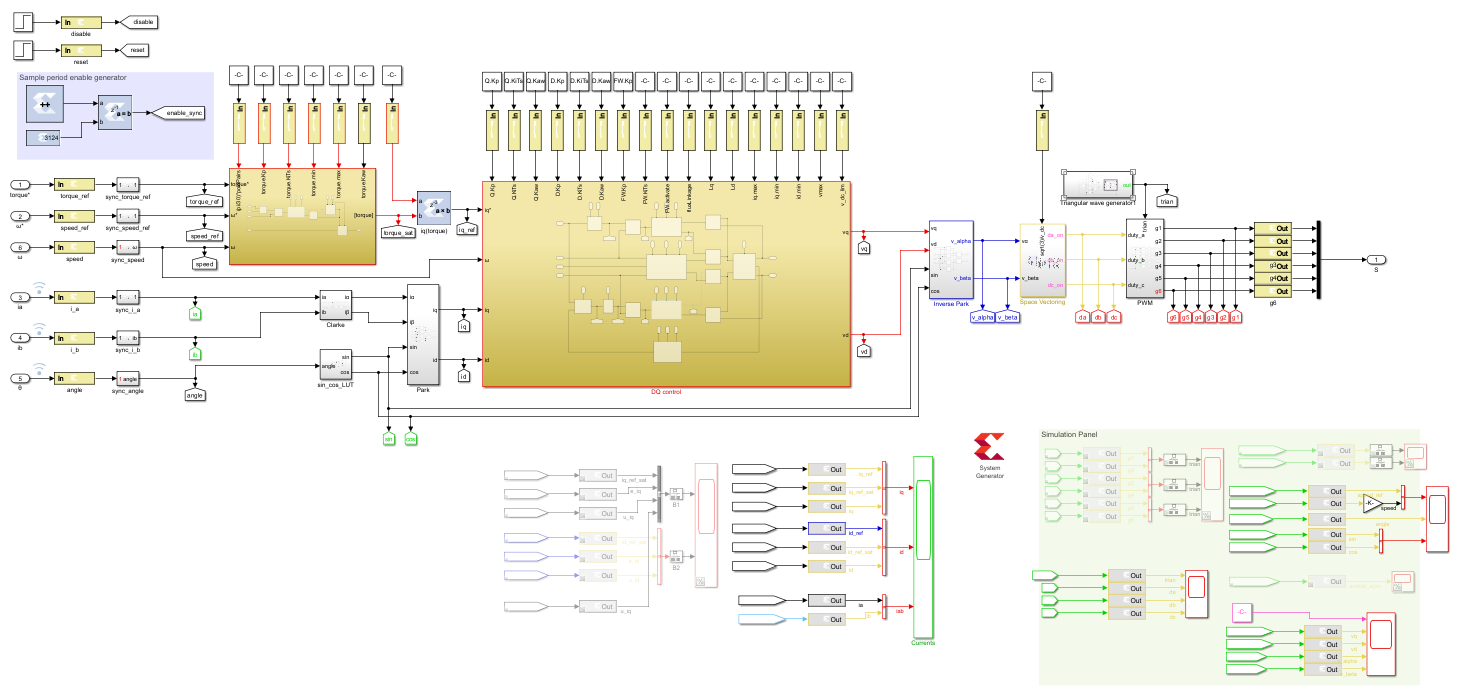
\includegraphics[width=16cm]
            { img/4_implementacio/control.png }
        \caption{ Implementació del control amb Vitis\texttrademark Model Composer }
    \end{figure}

    \subsubsection{ Controladors PI }
    { 
        L'algorisme fa servir un total de quatre controladors
        proporcionals-integrals (PI) ajustats manualment. S'ha decicit
        utilitzar controladors PI en comptes de PID perquè la part derivativa
        del control pot arribar a comportar-se erràticament en contextes amb
        molt de soroll. Els PI del control de corrent compten amb
        \emph{anti-windup}, ja que en cas contrari els PI calcularien els
        següents valors sense saber que la seva resposta està saturada. La
        tècnica de wind-up implementada consisteix a multiplicar per una
        constant l'error degut a la saturació i sumar-ho a l'acummulador del
        control integral \cite{pi_fpga}.

        \begin{figure}[!htb]
            \centering
            \captionsetup{justification=centering, margin=1.5cm}
            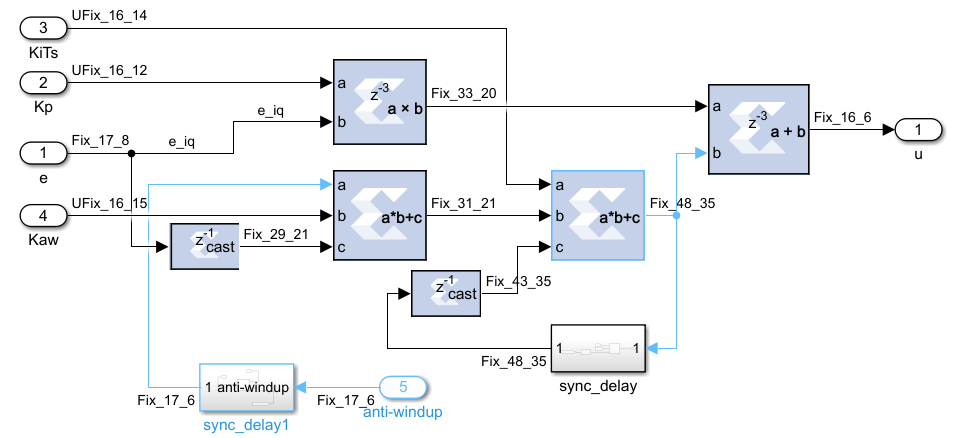
\includegraphics[width=11cm]
                { img/4_implementacio/PI_controller_id.png }
            \caption{ Detall de la implementació d'un PI amb \emph{anti-windup} }
        \end{figure}
    }

    \subsubsection{ Control de velocitat }
    { 
        La implementació del control de velocitat es basa en una doble
        saturació de la consigna de parell. L'estimació del límit superior del
        parell es realitza amb un controlador PI l'entrada del qual és l'error
        en la velocitat angular actual.

        \begin{figure}[!htb]
            \centering
            \captionsetup{justification=centering, margin=1.5cm}
            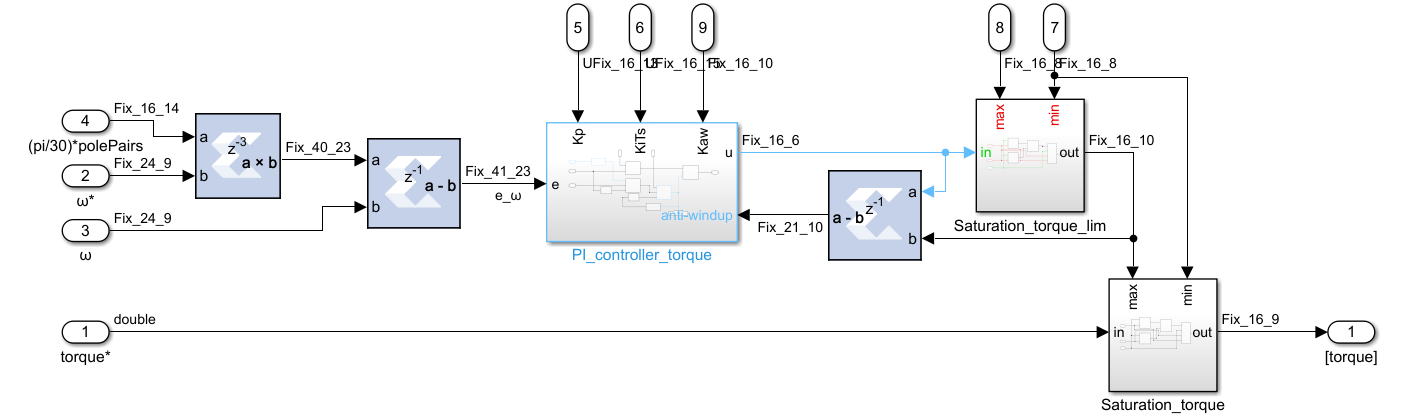
\includegraphics[width=14cm]
                { img/4_implementacio/speed_control.png }
            \caption{ Implementació del control de velocitat }
        \end{figure}
    }

    \subsubsection{ Sinus i cosinus }
    { 
        Per obtenir el sinus i el cosinus d'un angle donat, necessari per
        implementar la transformada i la antitransformada de Park, s'ha
        inclòs una look-up table amb els seus valors i una certa lògica
        addicional que permet la multiplexació de la lookup table per obtenir
        simultàniament ambdues funcions trigonomètriques.

        \begin{figure}[!htb]
            \centering
            \captionsetup{justification=centering, margin=1.5cm}
            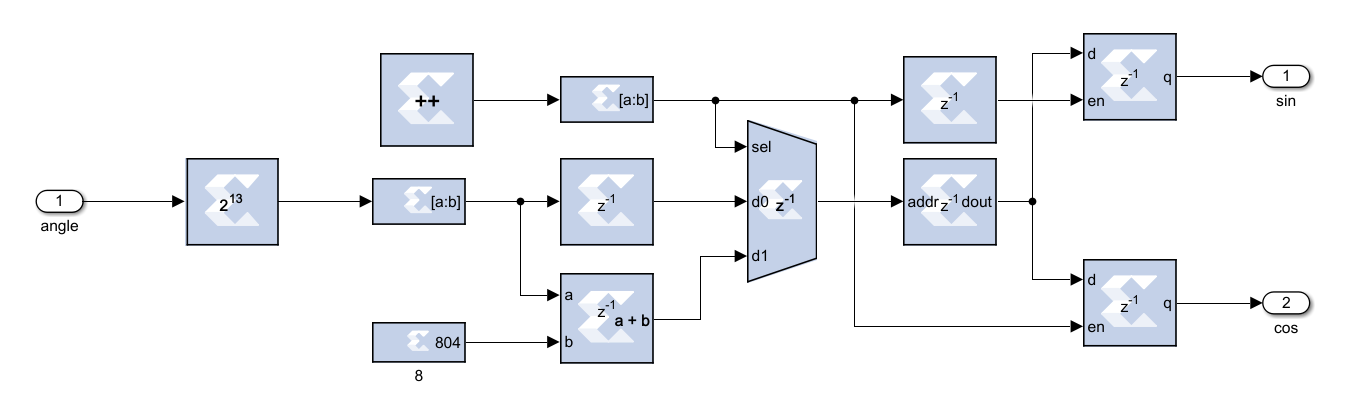
\includegraphics[width=12cm]
                { img/4_implementacio/sineLUT.png }
            \caption{ Implementació de les funcions sinus i cosinus }
        \end{figure}
    }

    \subsubsection{ Transformades de Clarke i de Park }
    { 
        La implementació de la transformada de Clarke és relativament senzilla,
        ja que es tracta d'una transformació lineal. Per tant, es pot expressar
        en termes de sumes i multiplicacions. És convenient recalcar que la
        multiplicació per una potència de 2 no comporta penalització de
        recursos de hardware utilitzats, ja que en aritmètica de coma flotant
        aquesta operació es pot realitzant simplement reinterpretant la
        posición de la coma fixa.

        La transformada de Park, per la seva banda, s'ha implementat amb quatre
        blocs multiplicadors i 2 blocs sumadors-restadors.

        \begin{figure}[!htb]
            \centering
            \begin{minipage}[c]{7cm}
                \centering
                \captionsetup{justification=centering}
                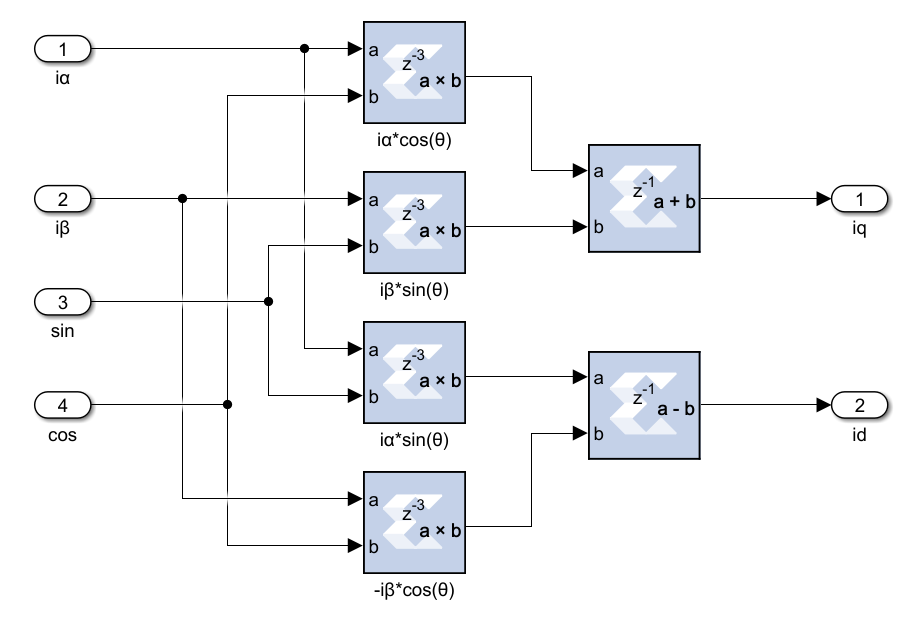
\includegraphics[width=7cm]
                    { img/4_implementacio/park.png }
                \caption{ Implementació de la transformada de Park }        
            \end{minipage} \hfil
            \begin{minipage}[c]{7cm}
                \centering
                \captionsetup{justification=centering}
                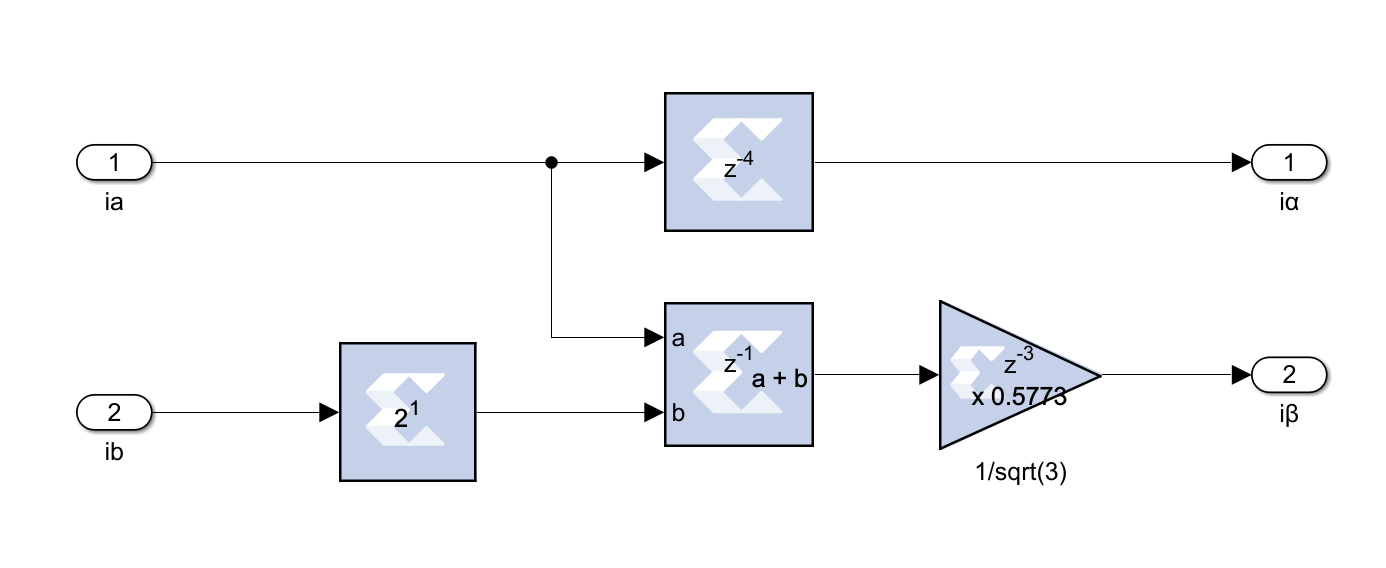
\includegraphics[width=7cm]
                    { img/4_implementacio/clarke.png }
                \caption{ Implementació de la transformada de Clarke }           
            \end{minipage} \hfil
        \end{figure} 
    }

    \subsubsection{ Control de corrent }
    { 
        Per al control de corrent s'han implementat dos controladors
        proporcionals-integrals (PI) ajustats manualment. En el mateix bloc
        també s'han implementat les funcions de desacoblament i de el limitador
        de voltatge, que limita la magnitud del voltage; així com les
        corresponents al Field Weakening i el MTPA.

        \begin{figure}[!htb]
            \centering
            \captionsetup{justification=centering, margin=1.5cm}
            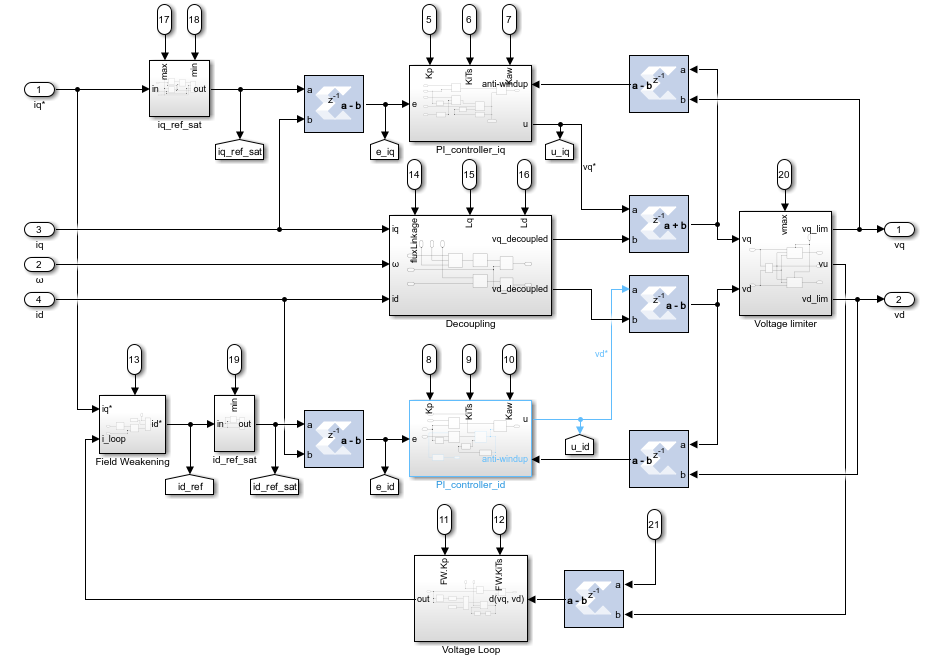
\includegraphics[width=12cm]
                { img/4_implementacio/current_control.png }
            \caption{ Vista general del bloc de control de corrent }
        \end{figure}
    }

    \subsubsection{ Field Weakening }
    { 
        El debilitament de camp s'implementa com un llaç de control tancat amb
        un controlador PI semblant als del control de corrent. No obstant,
        compta amb una condició inicial que ha de complir per activar el seu
        funcionament. Per tal d'activar el Field Weakening, per una banda, la
        velocitat ha de ser superior a la velocitat base, que és de 9000 rpm, i
        per l'altra, el voltatge de referència calculat ha de ser superior al
        de bus DC. Aquest bloc es pot desactivar si el senyal FW.activate es
        posa a 0.
    
        \begin{figure}[!htb]
            \centering
            \captionsetup{justification=centering, margin=1.5cm}
            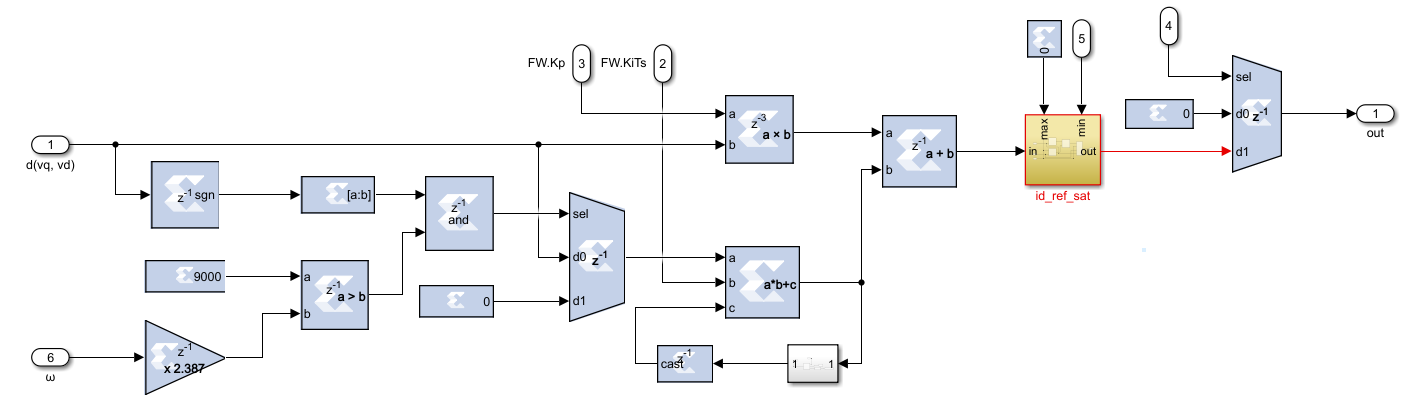
\includegraphics[width=14cm]
                { img/4_implementacio/fw.png }
            \caption{ Implementació del Field Weakening }
        \end{figure}
    }

    \subsubsection{ MTPA i generació de la referència $i_d*$ }
    { 
        El bloc de generació de la referència de corrent $i_d*$ rep a les
        entrades del llaç de voltatge del Field Weakening i realitza el càlcul
        del MTPA. L'equació de MTPA s'ha implementat per mitjà d'una look-up
        table i, a l'igual que el bloc de FW, compta amb un multiplexor per
        activar o desactivar aquesta estratègia de control.

        \begin{figure}[!htb]
            \centering
            \captionsetup{justification=centering, margin=1.5cm}
            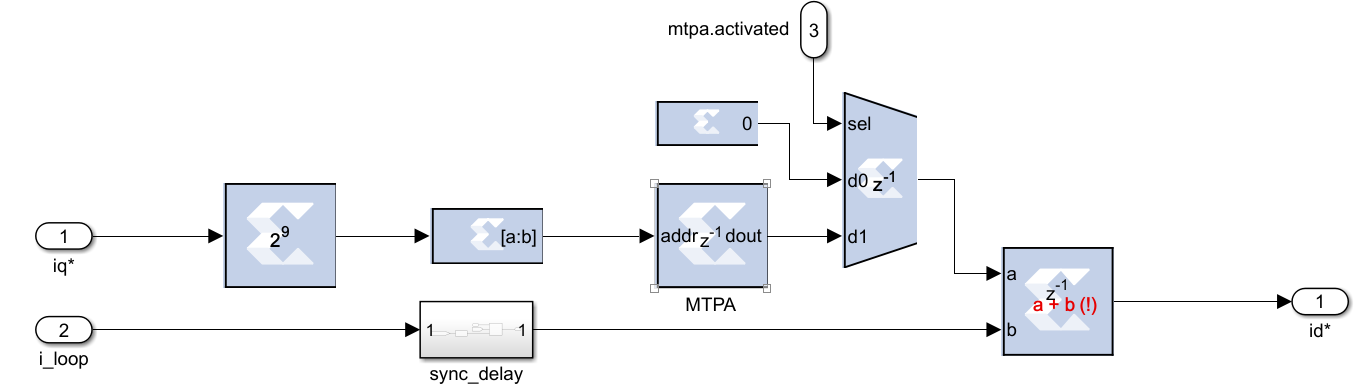
\includegraphics[width=12cm]
                { img/4_implementacio/mtpa.png }
            \caption{ Implementació de la generació del corrent de referència $i_d*$ }
        \end{figure}
    }

    \subsubsection{ Space Vector Modulation }
    { 
        En la figura \ref{ svpwm_fpga } es pot veure que s'han agrupat el
        diferents blocs per funcionalitat. Així, a la part superior, tenim la
        identificació del sector com tres condicions i un bloc concatenador;
        baix a l'esquerra estàn els multiplicadors que realitzen la
        normalització del vector de referència; a la seva dreta, es troben els
        blocs amb els quals obtenim les variables X, -X, Y, -Y, Z i -Z, i
        finalment els blocs generadors dels temps $t_1'$, $t_2'$ i $t_0$,
        associent-los a la fase corresponent de l'inversor per mitjà de tres
        multiplexors. 

        \begin{figure}[!htb]
            \centering
            \captionsetup{justification=centering,margin=1.5cm}
            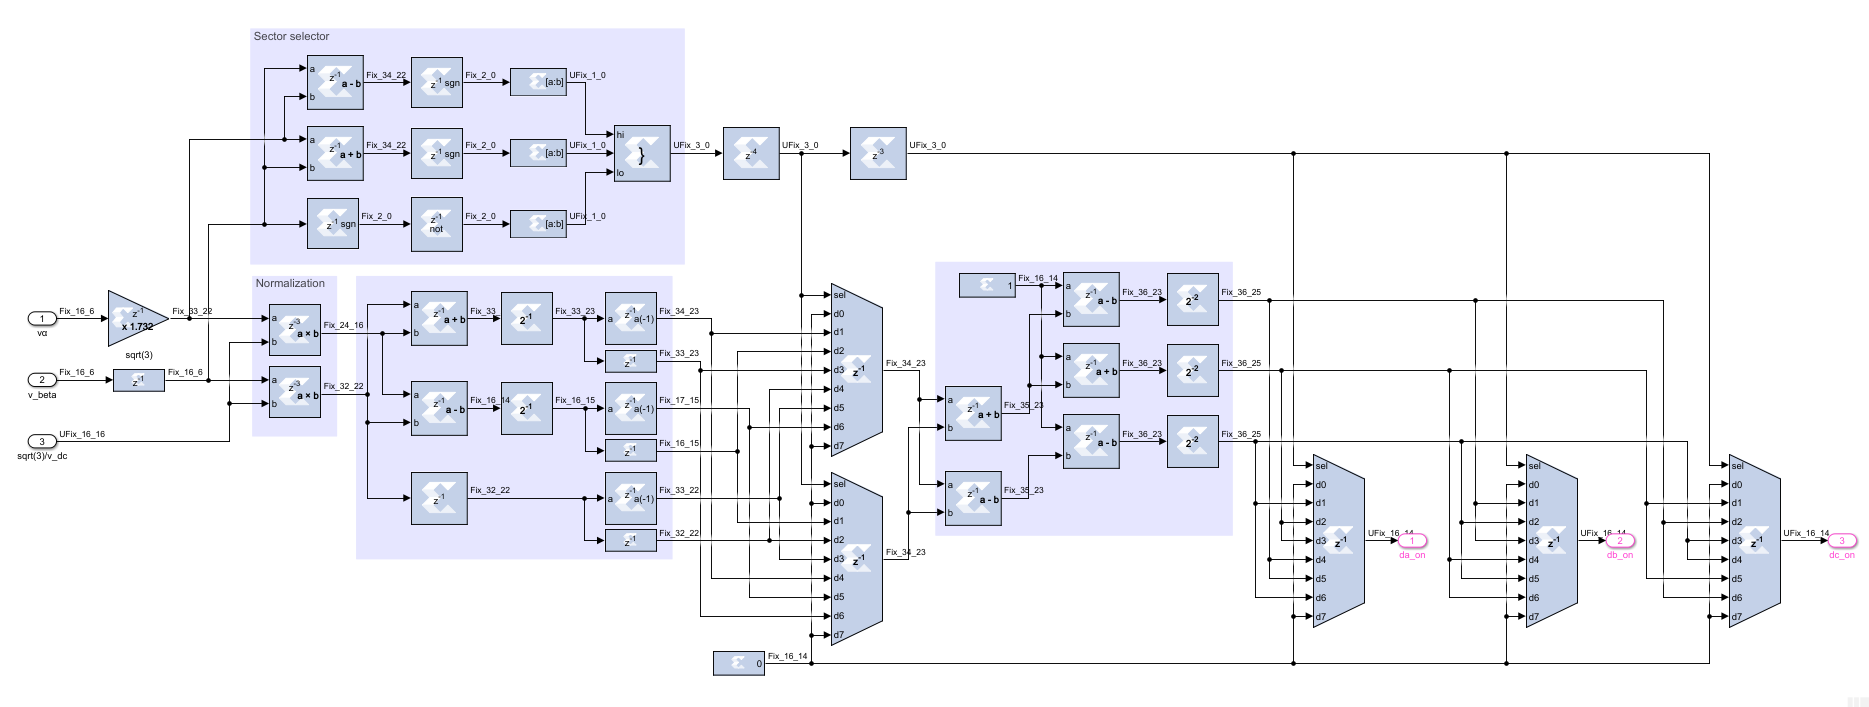
\includegraphics[width=16cm]
                { ../img/4_implementacio/sv.png }
            \caption{ Implementació de l'SVPWM. }
            \label{ svpwm_fpga }
        \end{figure}
    }

    \subsubsection{ Generació de PWM }
    {
        Per generar els senyals de commutació del transistor es comparen els
        tres cicles de treballs aconseguits mitjançant la modulació SV amb una
        portadora triangular. Cada comparació dóna lloc a dos senyals PWM
        contraposats, una l'inversa de l'altre, que corresponen als temps
        d'encesa i d'apagada dels dos transistors d'una fase de l'inversor. És
        important generar un petit temps entre els flancs de pujada i de
        baixada de les tensions de porta del transistors, ja que els pendents
        no són ideals; és el que es coneix com \emph{deadtime}. En el nostre
        cas, implementem un \emph{deadtime} d'$1 \mu s$.

        \begin{figure}[!htb]
            \centering
            \begin{minipage}[c]{7cm}
                \centering
                \captionsetup{justification=centering}
                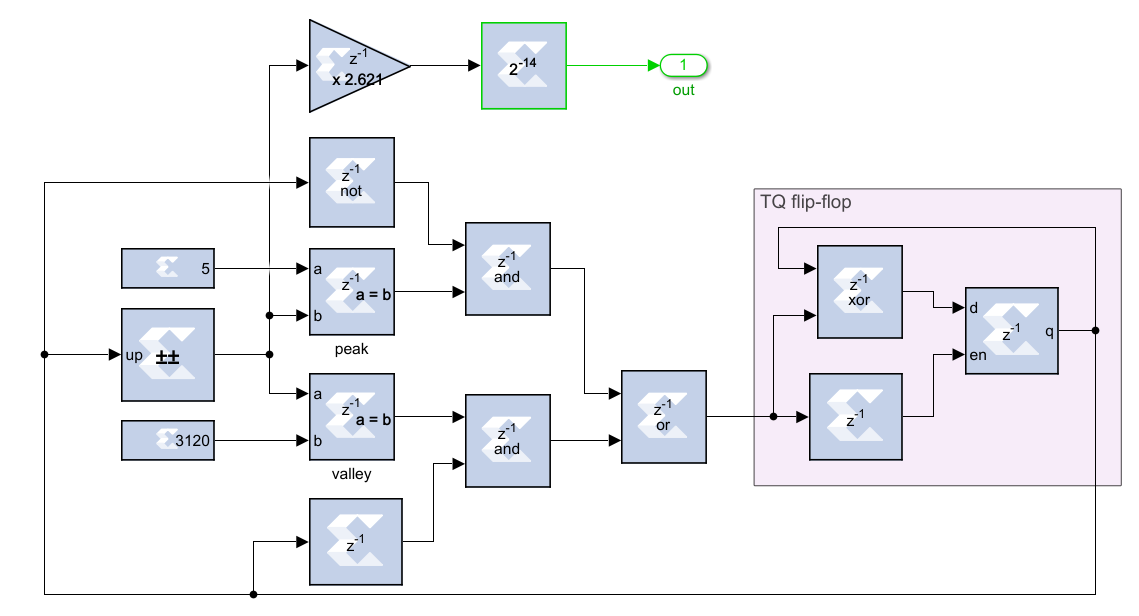
\includegraphics[width=7cm]
                    { img/4_implementacio/triangular.png }
                \caption{ Bloc de generaciió de la portadora triangular }                
            \end{minipage} \hfil
            \begin{minipage}[c]{7cm}
                \centering
                \captionsetup{justification=centering}
                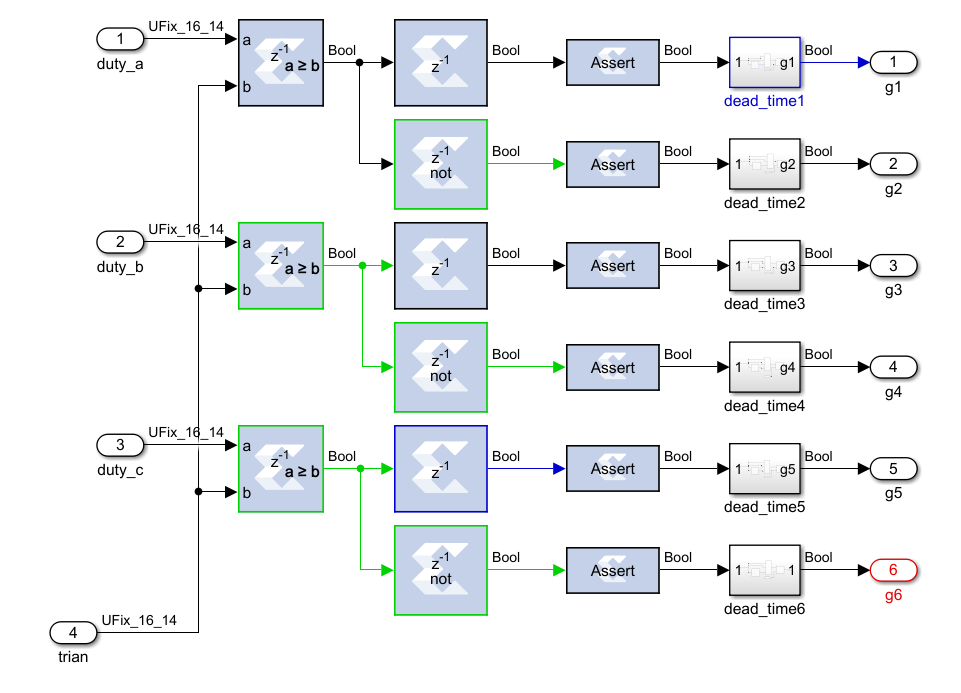
\includegraphics[width=7cm]
                    { img/4_implementacio/pwm.png }
                \caption{ Bloc de generaciió de PWM }                
            \end{minipage} \hfil
        \end{figure} 
    }
}

\subsection{ Implementació de la lògica programable }
{ 
    Un cop validat l'algorisme de control en
    \emph{Matlab/Simulink\textsuperscript{\textregistered}}, s'exporta el model
    a IP de \emph{Vivado}, l'eina de Xilinx per a la programació de les seves
    FPGAs. Les IP (\emph{Intelectual Property}) de \emph{Vivado} són
    subsistemes desenvolupats en aquesta eina que poden ser emprats en altres
    projectes. Xilinx disposa d'una extensa llibreria d'IPs que poden ser
    utilitzades per reduir l'esforç de disseny i el \emph{time to market}.

    Directament des del bloc \emph{System Generator} de \emph{Vitis Model
    Composer} es pot afegir la configuració per generar IPs. En tenir-ho, s'ha
    d'integrar la IP en un projecte de \emph{Vivado}. Per provar les
    funcionalitats de l'algorisme de control sobre la placa, s'ha realitzat el
    següent disseny de blocs de Vivado:

    \begin{figure}[!htb]
        \centering
        \captionsetup{justification=centering,margin=1.5cm}
        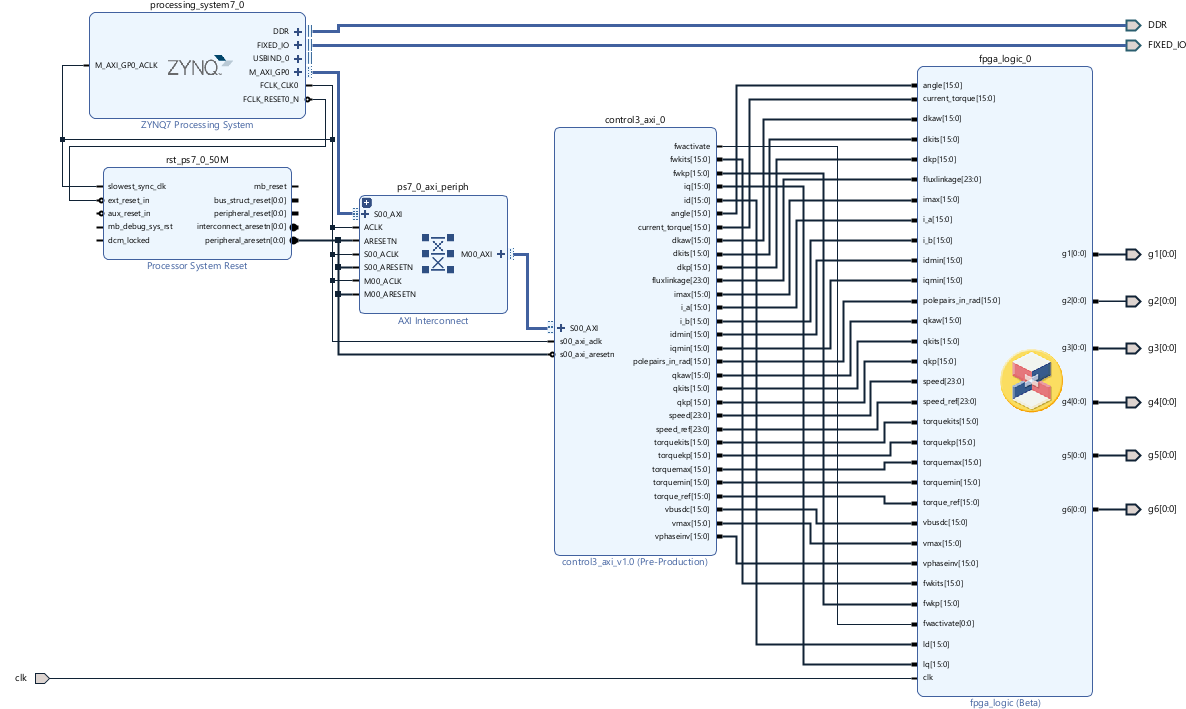
\includegraphics[width=15.5cm]
            { img/4_implementacio/vivado.png }
        \caption{ Disseny de blocs en el projecte de Vivado }
    \end{figure}

    En el cantó superior esquerra es troba el bloc que configura el processador
    del SoC Zynq. Just a la dreta del bloc de reset es troba el bloc que permet
    l'ús del bus \ac{AXI} de comunicació entre la lògica programable i el
    processador. Per configurar els registres del bus \ac{AXI} es fa servir l'IP
    customitzada \emph{control3\_axi} que actua com un perifèric del bus \ac{AXI}.
    Finalment, a la dreta tenim el bloc generat mitjançant l'eina \emph{Vitis
    Model Composer} i que conté l'algorisme desenvolupat.

    Seguint el flux de treball de Vivado, s'ha de realitzar la síntesi i la
    implementació del disseny. Els resultats de la implementació s'adjunten a
    l'annex \ref{vivado}.
}

\subsection{ Implementació del sistema d'arrencada i parada }
{ 
    El sistema d'arrencada i parada s'ha implementat com una aplicació escrita
    en llenguatge C++ que corre a sobre d'una distribució específica de Linux.

    \subsubsection{ Linux }
    { 
        La distribució implementada per al projecte es coneix com PetaLinux,
        està desenvolupada per Xilinx i és específica dels SoCs de la família
        Zynq-7000. 
        
        Linux permet abstreure el desenvolupament d'aplicacions del hardware
        que el suporta. Això es converteix en un avantatge si es vol aconseguir
        flexibilitat en quan a implementació, cosa ques es donaria, per
        exemple, si es vol canviar de SoC en un futur. Linux també permet una
        progamació concurrent ``multithreading" estàndard i ben definida \cite{cpp}.

        No obstant això, al contrari del que pensava l'autor, la implementació
        de Linux ha acabat resultant tot un repte. El principal impediment que
        s'ha trobat és trobar la configuració adequada dels fitxers de
        construcció de PetaLinux, ja que per una part les imatges del sistema
        operatiu per la Cora Z7-10 no són modificables amb la última versió de
        PetaLinux, i per l'altre, la versió antiga de PetaLinux compta amb
        moltes dependències que requereixen versions antigues i difícils de
        trobar.
    }

    \subsubsection{ C++ }
    { 
        La programació d'aplicacions en Embedded Linux es realitza
        tradicionalment en llenguatge C o C++. Se solen utilitzar aquest dos
        llenguatges de programació perquè són ràpids, robustos (gràcies en part
        al tipificat estàtic) i la API del kernel de Linux està escrita en C.
        
        Entre aquestes dues opcions s'ha escollit el llenguatge de programació
        C++, ja que funciona com un superconjunt de C, admet diferents
        paradigmes de programació, compta amb una bona llibreria estàndard i té
        una gestió de les excepcions interessant.

        En C++, la idea original al darrere de la progamació orientada a
        objectes era crear tipus propis que extenguesin les capacitats dels
        tipus encastats (\emph{Built-in types}). En paraules del creador de C++,
        Bjarne Stroustrup, ``For me, the key idea was basically I could get my
        own types, and that's the idea that goes for into C++, where I can get
        more better types, more flexible types and more efficient types.'' 
        \cite{lex}
        
        Seguint aquesta filosofia, s'han definit les classes State i Register,
        que representen un estat de la màquina d'estats i un registre AXI de la
        FPGA, respectivament, i que es comporten com tipus encastats en
        haver-hi sobrecarregat els operadors (\emph{operator overload}).

        La programació orientada a objectes també aporta modularitat al
        desenvolupament de l'aplicació. En el nostre cas, la modularitat ha
        permès encapsular la gestió de la màquina d'estats i d'una interfície
        d'usuari en classes diferents. La interfície d'usuari està pensada per
        realitzar tests amb la placa d'una manera sencilla i eficient. Amb
        l'encapsulació en classes es fa possible intercanviar la interfície
        d'usuari per pantalla per una interfície de comunicació basada en CAN o
        inclús en Ethernet.

        Addicionlment, C++ compta amb una gestió de les excepcions força
        interessant, a diferència de C. No obstant és una eina que ha
        d'emprar-se només en casos excepcionals, ja que cada cop que es llença
        i captura una exepció, el programa torna a l'estat que tenia abans
        d'entrar en l'espai encapçalat per \lstinline{try} i delimitat entre
        claudàtors.
    }

    \subsubsection{ Arquitectura desenvolupada }
    {        
        Es fa servir el concepte extès de la màquina d'estats finita en
        software per controlar el flux del programa d'arrencada i d'aturada del
        motor. Els estats de la màquina d'estats es mostra en la figura
        \ref{fms_uml}

        \begin{figure}[!htb]
            \centering
            \captionsetup{justification=centering, margin=1cm}
            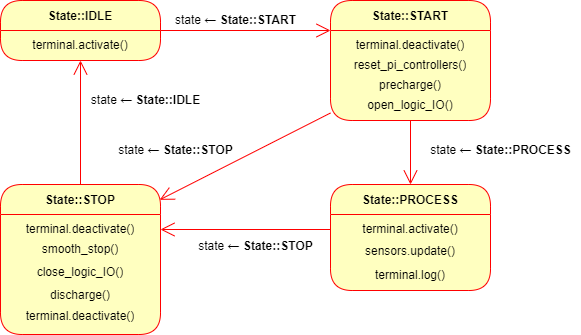
\includegraphics[width=10cm]
                { img/4_implementacio/state_machine.png }
            \caption{ Diagrama UML de la màquina d'estats finita.
             }
            \label{fms_uml}
        \end{figure}

        \paragraph{Main}
        {
            Representa el programa principal. En aquest mòdul s'hi defineix la
            funció principal del programa, en la que s'initzializen els
            registres AXI i es generen els \emph{threads} amb els
            \emph{handlers} de la màquina d'estats i la interfície de terminal,
            \lstinline{state\_loop()} i \lstinline{terminal\_loop()},
            respectivament.
        }
        
        \paragraph{State}
        { 
            En aquest mòdul s'han incorporat els mòduls relacionats amb la
            màquina d'estats. La instància de la classe \emph{State} representa
            un estat de la màquina d'estats. S'ha utilitzat una enumeració per
            descriure els estats. L'assignació de l'estat actual es realitza
            per mitjà de l'\lstinline{operator=()}. La seva implementació té en
            compte les possibles transicions i llança una excepció en el cas
            que es forci una transició que no és possible. El bucle que
            defineix la màquina d'estats s'ha implementat a la funció
            \lstinline{state_loop()}.

            \begin{figure}[!htb]
                \centering
                \captionsetup{justification=centering,margin=1.5cm}
                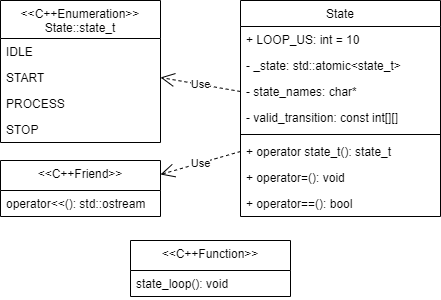
\includegraphics[width=7.5cm]
                    { img/4_implementacio/uml_state.png }
                \caption{ Diagrama UML del mòdul State.  }
            \end{figure}
        }

        \paragraph{Terminal} 
        { 
            En aquest mòdul s'hi defineix la interfície d'usuari amb el
            programa, en la qual l'usuari escriu les comandes per operar
            l'inversor. De manera paral·lela al mòdul State, s'ha creat una
            enumeració, en aquest cas amb les comandes possibles i una funció
            \lstinline{terminal_loop()}. 
            
            Així, les comandes \lstinline{Terminal::START} i
            \lstinline{Terminal::STOP} marquen el pas dels estats
            \lstinline{State::IDLE} a \lstinline{State::START} i de
            \lstinline{State::PROCESS} a \lstinline{State::STOP},
            respectivament. La comanda \lstinline{Terminal::EDIT} permet editar
            el valor dels registres AXI realitzant una cridada al programa de
            Linux $vi$. D'altra banda, les comandes \lstinline{Terminal::SPEED}
            i \lstinline{Terminal::TORQUE} permeten variar el valor de la
            velocitat i el parell durant l'estat \lstinline{State::PROCESS}.
            Finalment, \lstinline{Terminal::HELP} mostra un missatge d'ajuda i
            \lstinline{Terminal::UNKNOWN} és seleccionat en el cas que
            s'introdueixi una comanda no reconeguda.

            \begin{figure}[!htb]
                \centering
                \captionsetup{justification=centering,margin=1.5cm}
                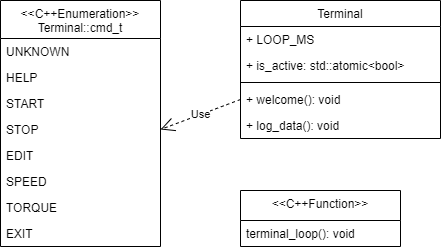
\includegraphics[width=7.5cm]
                    { img/4_implementacio/uml_terminal.png }
                \caption{ Diagrama UML del mòdul Terminal.  }
            \end{figure}
        }

        \paragraph{Register} 
        { 
            En aquest mòdul es defineixen, les classes Register i Sensor. La
            classe Register és una implementació a més alt nivell d'un registre
            del \ac{SoC}, en el que les lectures i les escriptures es
            converteixen de coma flotant a coma fixa i a l'inrevés, per a la
            seva interpretació per l'algorisme de control. La classe Sensor
            conté un Registre i en afegit incorpora la lògica per parar el
            funcionament de l'algorisme en cas que el sensor detecti que un
            registre sobrepassa un valor determinat, per exemple, de
            temperatura, voltatge o corrent.

            \begin{figure}[!htb]
                \centering
                \captionsetup{justification=centering,margin=1cm}
                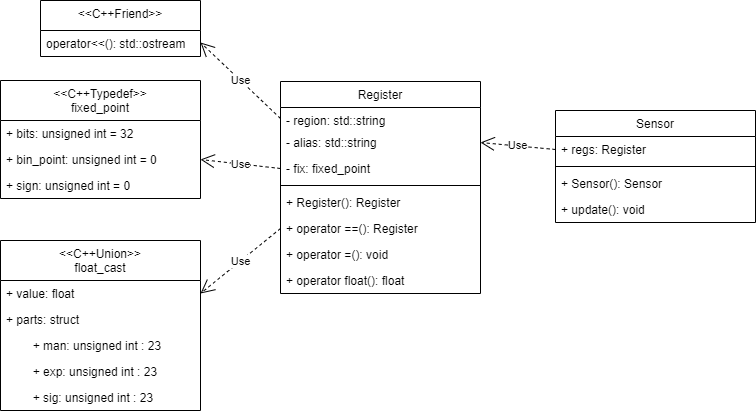
\includegraphics[width=11cm]
                    { img/4_implementacio/uml_register.png }
                \caption{ Diagrama UML de classes del mòdul Register.
                 }
            \end{figure}
        }

        \paragraph{Subroutines} 
        { 
            En aquest mòdul es defineixen les subrutines com funcions. Cada una
            d'elles realitza una sèrie de tasques, relacionades amb l'inversor.
            Aquestes subrutines no están implementades en el moment de
            l'escriptura de la memòria; sino que llençen una excepció
            notificant que no estan implementades. Les subrutines són les
            següents:

            \begin{itemize}

                \item \lstinline{void init_AXI_registers()}:
                    Initialitza els registres AXI de la lògica programable amb
                    els valors emmagatzemats a l'arxiu de paràmetres
                    \emph{param.txt}. Es crida quan s'inicia el programa i cada
                    cop que s'actualitza el contingut de \emph{param.txt}.

                \item \lstinline{void reset_pi_controllers()}:
                    Activa el senyal de reset dels blocs acumuladors dels
                    controladors PI. És una rutina bastant important que es
                    realitza.

                \item \lstinline{void precharge()}: 
                    Es comunica per bus CAN amb el microcontrolador de la placa
                    de precàrrega dels condensadors per notificar la intenció
                    d'iniciar el funcionament del motor i començar a
                    precarregar-los. Aquesta funció bloqueja la màquina
                    d'estats fins que acaba la precàrrega i rep el senyal
                    d'acabada.

                \item \lstinline{void discharge()}:
                    De manera semblant a la funció \lstinline{void precharge()}, estableix
                    comunicació amb el circuit de descàrrega, comença a
                    descarregar els condensadors i es bloqueja fins que acaba
                    la descàrrega, moment en el que rep el senyal d'acabada.

                \item \lstinline{void open_logic_IO()} i \lstinline{void close_logic_IO()}:
                    Aquestes funcions obren i tanquen els registres d'entrada i
                    de sortida de la lògica programable per iniciar el flux de
                    senyal a través de l'algorisme o per tancar-lo.
                    
                \item \lstinline{void change_speed(float speed)} i \lstinline{void change_torque(float torque)}:
                    Aquestes funcions canvien la consigna de velocitat i torque
                    de l'algorisme de control, respecivament, sempre que el
                    sistema es trobi en l'estat \lstinline{State::PROCESS}.

                \item \lstinline{void smooth_stop()}:
                    Realitza el protocol d'acabada suau per evitar que el
                    control finalitzi amb un esglaó.

            \end{itemize}
        } 

        \paragraph{Utils} 
        { 
            El mòdul Utils conté funcions i classes relacionades amb el flux del
            programa com són la classe Log i la funció exit program. En
            instanciar un objecte de la classe Log es mostra per pantalla
            informació, errors o advertències, i són habitualment llençades com
            com excepcions. En el mateix mòdul estàn definides les macros INFO,
            WARNING i ERROR per simplificar la seva implementació en el codi.
            D'altra banda, la funció \lstinline{exit_program()} comença a gestionar la
            sortida del programa en el cas que sigui possible. També és
            utilitzada per sobreescriure el \emph{handlers} dels senyals
            SIGNINT i SIGNTERM per evitar sortides del programa accidentals.
        
            \begin{figure}[!htb]
                \centering
                \captionsetup{justification=centering, margin=1.5cm}
                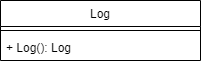
\includegraphics[width=3.8cm]
                    { img/4_implementacio/uml_log.png }
                \caption{ Diagrama UML de classes del mòdul Log. }
            \end{figure}
        } 
    }
}

\subsection{ Comunicació CAN }
{ 
    La comunicació pel bus CAN es realitza per mitjà del connector CAN de la
    placa Z-Turn. El packet SocketCAN del kernel de Linux proporciona els
    drivers necessaris per implementar diferents protocols de comunicació per
    CAN. La \ac{API} de SocketCAN per programar en C/C++, Linux-CAN, està basada en la Berkeley socket API, que
    té com avantatges ser independent del hardware i ser un estàndard prou
    utilitzat, amb la qual cosa es pot aprofitar l'extensa documentació al
    respecte per programar aplicacions com poden ser els populars servidors i
    clients TCP/IP \cite{can-utils} \cite{socketCAN}.

    S'ha dissenyat una prova per validar la implementació de CAN.
    Malauradament, el retràs en la comanda de la placa de la FPGA ha dificultat
    la validació de la comunicació per CAN, ja que la placa Cora Z-7 de la que
    es disposa no compta amb connector CAN i s'ha d'adaptar amb un hardware
    específic adicional (PmodCAN) que no està previst fer servir per la
    implementació de l'inversor.

    Per començar a desenvolupar amb la llibreria Linux-CAN, en un primer lloc,
    s'ha d'incloure la llibreria \lstinline{#include <linux/can.h>}. Un cop
    iniciat, s'ha de crear i configurar un descriptor de fitxer (\emph{file
    descriptor}) mitjançant la crida a la funció \lstinline{socket()},
    \lstinline{setsockopt()} i \lstinline{ioctl()}. Després de lligar el
    descriptor de fitxer a l'adreça del CAN amb \lstinline{bind()}, ja es pot
    començar a enviar dades amb les crides a \lstinline{write()} i
    \lstinline{read()}.
}

\clearpage \section{Experiments i resultats}
Els experiments per validar la implementació de l'algorisme han estat limitats
per diferents factors. En primer lloc, ha estat difícil aconseguir una bona
validació del funcionament de l'algorisme en Simulink perquè les simulacions
són bastant lentes, degut a que Vitis Model Composer imposa un període
del solver igual o inferior al període de rellotge escollit. Una solució
possible és realitzar un model del motor en FPGA a mode de \emph{hardware in
the loop}. Malauradament, es decidí no implementar aquest experiment en l'abast
d'aquest projecte i provar d'implementar el control directament sobre la FPGA i
realitzar les proves directament amb les plaques de potència, cosa que
finalment no s'ha aconseguit.

\subsection { Test unitaris }
{
    S'han realitzat una sèrie de tests unitaris de diversos components de
    l'algorisme per testejar el seu funcionament.

    \paragraph{Sinus i cosinus} S'introdueix un senyal dent de serra a
        l'entrada del subsistema i es compara el resultat amb un bloc de
        generació de sinus i cosinus nadiu de Simulink. La freqüència del
        senyal a l'estrada és molt major a la que s'emprarà en realitat; però,
        ens permet fer-nos una idea del retard (delay) de l'operació i de la
        resolució temporal, en el nostre cas dos vegades el periode de rellotge
        del sistema.

        \begin{figure}[!htb]
            \centering
            \captionsetup{justification=centering,margin=1.5cm}
            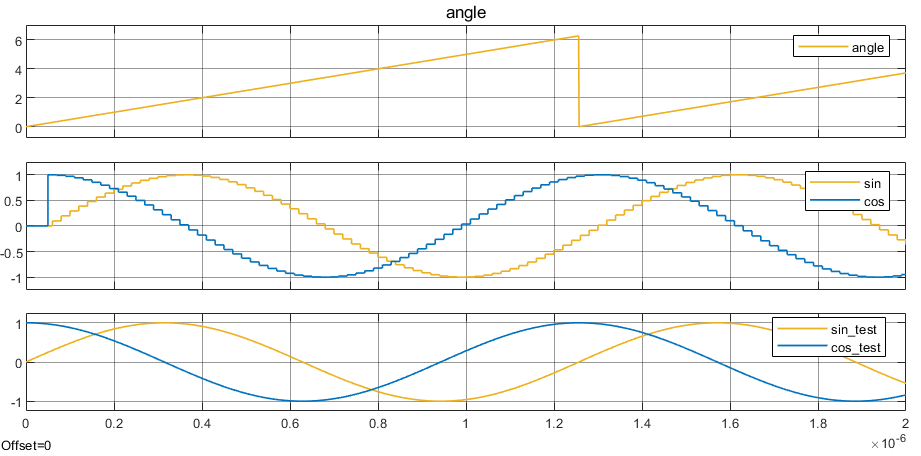
\includegraphics[width=8cm]
                {img/5_resultats/sineLUT_test.png}
            \caption{ Prova de la implementació del sinus i del cosinus }
        \end{figure}
    

    \paragraph{Senyal triangular} Es pot veure en aquest test que senyal
        triangular del PWM es genera a la freqüència correcta i l'amplitud en
        coma fixa s'intrpreta correctament.
    
        \begin{figure}[!htb]
            \centering
            \captionsetup{justification=centering,margin=1.5cm}
            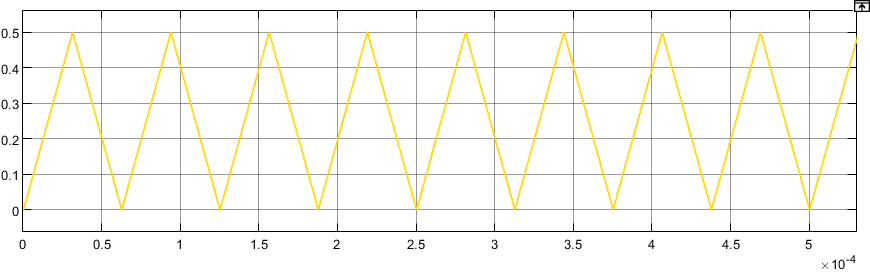
\includegraphics[width=8cm]
                {img/5_resultats/triangular.png}
            \caption{ Prova de la implementació del senyal triangular pel PWM }
        \end{figure}     
    

    \paragraph{SVPWM} Per a la prova del SVPWM, s'introduix com entrada dos
        senyals sinusoidals desfasats 90º. Simulem així un vector espacial de
        magnitud i frqüència de rotació constant i obtenim la forma d'ona
        característica de l'SVPWM.

        \begin{figure}[!htb]
            \begin{minipage}[c]{7.5cm}
                \centering
                \captionsetup{justification=centering}
                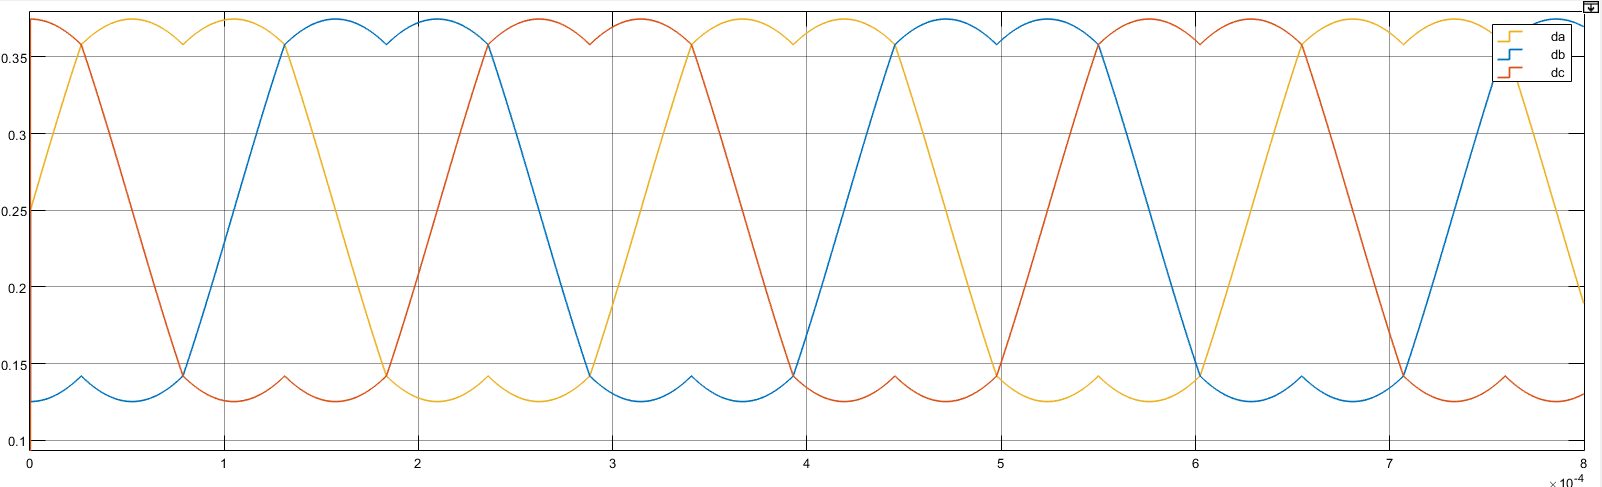
\includegraphics[width=7cm]
                    {img/5_resultats/sv_test.png}             
            \end{minipage} \hfil \hfil
            \begin{minipage}[c]{7.5cm}
                \centering
                \captionsetup{justification=centering}
                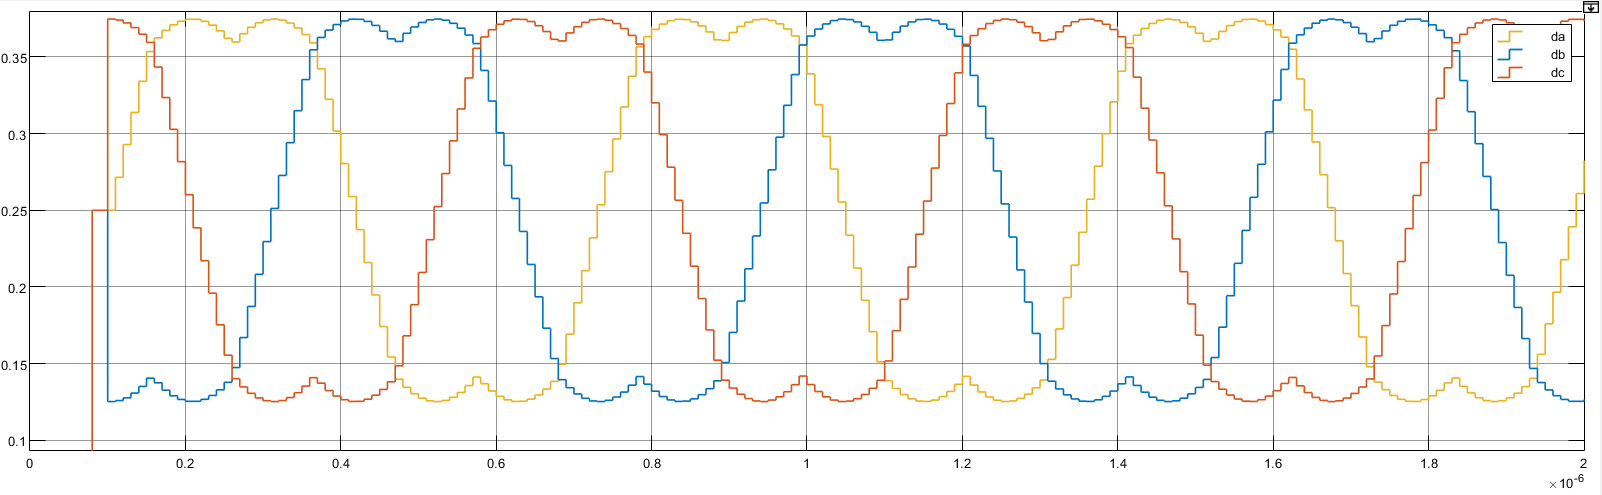
\includegraphics[width=7cm]
                    {img/5_resultats/sv_test2.png}           
            \end{minipage} \hfil
            \caption[Proves d'implementació de l'SVPWM]
            {  
                Proves d'implementació de l'SVPWM. A la dreta la 
                freqüència del senyal s'apropa molt més a la freqüència de
                rellotge del sistema.
            }
        \end{figure} 
        
    \paragraph{Limitador de voltatge} S'excita el bloc amb un senyal en rampa
        de $v_d$ i $v_q$ i s'observa que es limita el voltatge quan la magnitud
        del vector $v$ supera els $\frac{V_{DC}}{\sqrt{3}}$.
    
        \begin{figure}[!htb]
            \centering
            \captionsetup{justification=centering,margin=1.5cm}
            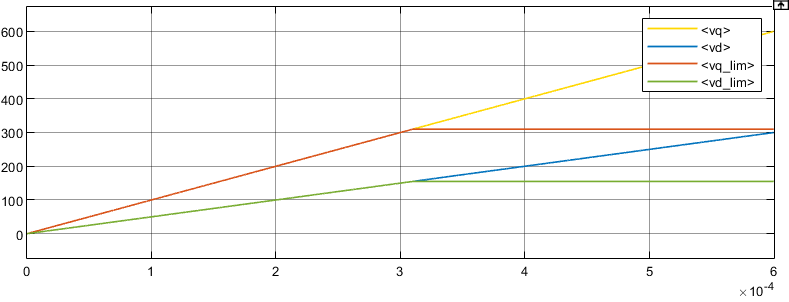
\includegraphics[width=7.5cm]
                {img/5_resultats/limitador.png}
            \caption{ Prova de la implementació del limitador de voltatge }
        \end{figure}     
    
}

\subsection{Simulacions de l'algorisme complet}
{
    En aquest subapartat s'analitzen les prestacions de l'algorisme de control
    implementat en el seu conjunt. Per provar la implementació realitzada es
    substitueix l'algorisme en el model de Simulink desenvolupat per l'equip.
    El model de l'inversor és el commutat i el model de l'inversor s'implementa
    a partir de les equacions del motor en el sistema de referència $d\-q$. És
    per això que s'implementen la transformada i la transformada inversa
    de Park a l'interior del subsistema del motor. 

    \begin{figure}[!htb]
        \centering
        \captionsetup{justification=centering,margin=1cm}
        \includegraphics[width=11cm]
            {img/5_resultats/control.png}
        \caption[Model de Simulink desenvolupat per l'equip]{ Model de Simulink desenvolupat per l'equip, on el bloc de control ha set substituit per la implementació en FPGA. }
    \end{figure}

    \subsubsection{ Resultats de la simulació }
    {
        Si realitzem una simulació de la implementació del control en Simulink,
        podem veure com obtenim una rotació accelerada del rotor.

        \begin{figure}[!htb]
            \centering
            \captionsetup{justification=centering,margin=1.5cm}
            \includegraphics[width=6cm]
                {img/5_resultats/angle.png}
            \caption{ Angle del rotor respecte l'estàtor. }
        \end{figure}

        Per accelerar lleugerament la simulació, feim una decimació dels
        punts emmagatzemats per Simulink. Obtenim els resultats següents:
        
        \begin{figure}[!htb]
            \centering
            \captionsetup{justification=centering,margin=1.5cm}
            \includegraphics[width=10cm]
                {img/5_resultats/test.png}
            \caption[Resultat de la simulació (I)]{
                Resultat de la simulació. A dalt hi tenim la referència de
                velocitat i la velocitat real. Enmig tenim l'evolució de l'angle
                amb el temps. Abaix tenim l'evolució del sinus i del cosinus de
                l'angle.
            }
        \end{figure}

        \begin{figure}[!htb]
            \centering
            \captionsetup{justification=centering,margin=1.5cm}
            \includegraphics[width=8cm, height=5cm]
                {img/5_resultats/Untitled.png}
            \caption[Resultat de la simulació (II)]{
                Resultat de la simulació. A dalt hi tenim la referència de
                corrent $i_q*$ i el corrent $i_q$; just a sota el mateix pel
                corrent $i_d$. Abaix tenim l'evolució dels corrents $i_a$ i $i_b$
                (marc de referència de l'estator).
            }
        \end{figure}
    }
}

\clearpage \section{Estudi econòmic} %i impacte mediambiental}
El pressupost total del projecte s'adjunta en la taula de sota. En el projecte
s'ha utilitzat tant la llicència d'estudiant de Matlab que proporciona la UPC
als seus estudiant com el període de prova de Vitis Model Composer de 3 mesos.
Així, es considera en la taula el cost que tindria el projecte sense tenir en
compte aquests conceptes.

\begin{table}[!htb]
    \caption{Cost del projecte}

    \begin{tabular}{l r l l r}
        \toprule
            \textbf{Concepte} & 
            \textbf{Preu} & 
            \textbf{Amortització} & 
            \textbf{Temps} & 
            \textbf{Cost total} \\
        \midrule
        
            MYIR Z-Turn & 
            187,72€ & 
            - & 
            - &
            187,72€ \\

            Portàtil MSI Leopard GP65 & 
            1299€ &
            1 mes &
            4 mesos &
            108,25€ \\

            Llicència Matlab & 
            800€/any &
            1 any &
            4 mesos &
            266,67€ \\

            Llicència Vitis Model Composer & 
            700€ &
            3 anys &
            3 mesos &
            43,75€ \\

            Sou enginyer & 
            10€/h &
            - &
            450 h &
            4.500€ \\
        \midrule
            {} & {} & {} & {\textbf{Total}} & {5106,39€} \\
        \cline{4-5}
    \end{tabular}
\end{table}

Per aquest projecte també es considera rellevant realitzar una traçabilitat
del programari emprat. D'aquesta manera, s'adjunta el Software Bill of
Materials en la forma de taula \ref{sbom}.

\begin{table}[!htb]
    \caption{ Software Bill of Materials  }
    \label{sbom}

    \begin{tabular}{l l m{6.4cm} m{3cm}}
        \toprule
            \textbf{Programari} & 
            \textbf{Versió} & 
            \textbf{Llicència} & 
            \textbf{Copyright} \\
        \midrule
            Matlab/Simulink & 
            2022a & 
            Entorn de simulació & 
            MathWorks \\

            Vivado &
            2021.2 &
            Disseny i implementació de lògica programable per FPGAs de Xilinx &
            AMD (Xilinx) \\

            Vitis &
            2021.2 &
            IDE de Xilinx basat en Eclipse &
            AMD (Xilinx) \\

            Vitis Model Composer & 
            2021.2 & 
            Extensió de Simulink & 
            AMD (Xilinx) \\ 

            PetaLinux & 
            2017.4 & 
            Distribució de Linux per la familia de SoCs ZYNQ-7000 & 
            AMD (Xilinx) \\ 

            CMake & 
            3.16.3 & 
            Generació de Makefiles per compilar C++ & 
            Kitware Inc. \\ 

            G++ & 
            9.4.0 & 
            Eina de compilació de C++ & 
            Free Software Foundation Inc. \\ 

        \bottomrule
    \end{tabular}
\end{table}

% \clearpage \section{ Impacte mediambiental }
% \input{ sections/y_environment.tex }

\clearpage \section{Conclusions}
En aquesta memòria s'ha explicat i analitzat el procés d'implementació d'un
control per \emph{Motor drive} en FPGA i de la capa de seguretat addicional,
posant especial èmfasi a les decisions presses en cada moment i com s'ha anat
desenvolupant el projecte en conseqüència. 

El projecte va iniciar-se amb bon peu en un principi. En la fase
intermitja es varen trobar algunes dificultats en la depuració del model en
Vitis Model Composer, en gran part pels temps de simulació elevats. Es va poder
completar aquest apartat; no obstant, els resultats obtinguts no acaben de ser
totalment rigurosos. En el cas d'haver-hi dedicat un temps addicional a
l'experimentació i l'anàlisi dels resultats en comptes de continuar amb la capa
de programari, es podria haver acabat de validar completament l'algorisme en
FPGA. No obstant, es decidí seguir amb el pla de treball original, ja que en el
moment de realitzar la revisió crítica es va subestimar la magnitud del treball
necessari per programar la capa d'arrencada, parada i seguretat, evidenciat en
aspectes com la dificultat de la implementació de la comunicació per bus CAN a
causa dels problemes de compatibilitat sorgits.

D'altra banda, l'ús de l'eina Vitis Model Composer ha resultat en bona mesura una
decisió acertada. Tanmateix, han sorgit certes dificultats que han empitjorat
el temps de depuració de l'algorisme:

\begin{itemize}

    \item \textbf{Paràmetres ocults.}
        Certa configuració que es troba oculta a primera vista, com és la
        configuració de la coma fixa o el \emph{sample rate} de cada bloc, amb
        la qual cosa es dificulta en certa mesura la depuració.

    \item \textbf{Bloqueig de Matlab.} 
        En realitzar les simulacions, moltes vegades Matlab es bloquejava i
        s'havia d'iniciar el programa des del principi, cosa que comportava una
        possible pèrdua de les dades.

    \item \textbf{Dificultat amb el control de versions.}
        El control de versions no es aplicable amb els fitxers \emph{.slx} que
        contenen la configuració dels models de Simulink, ja que no estan
        pensats per comparar-los a nivell de codi. En conseqüència, el
        control de versions amb eines com Git es coplica ja que no podem
        accedir i modificar les línies de codi que el configuren.

\end{itemize}

Finalment, volia destacar que personalment aquest projecte ha suposat un procés
d'aprenentatge constant, no només a nivell tècnic i d'assimilació de nous
conceptes sinó també a nivell d'autoconeixement, organització personal i gestió
de les expectatives. He après bastant entenent el per què no he pogut
aconseguir certes fites en el projecte que no aplicant el conceptes que ja
tenia, sense deixar de valorar la feina realitzada i la constància aplicada.
Puc dir amb seguretat que l'experiència obtinguda treballant aquest projecte
m'ajudarà en un futur a afrontar reptes més complexos i exigents.

\clearpage \section{Treball futur}
Com ja s'ha vist al llarg de la memòria, encara queda treball per realitzar
tant a nivell de programari com de hardware. Així, el projecte del \emph{motor
drive} propi encara continua i es preveuen avenços en els propers mesos. En el
moment de l'escriptura de la memòria, l'equip està iterant el disseny les
plaques de potència, que es el pas previ al seu montatge i testeig físic. 

Quant l'implementació de l'algorisme de control i de la capa de seguretat es
poden destacar els següent treball futur:

\begin{itemize}
    \item 
        S'implementarà i es validarà la comunicació CAN amb els circuits de
        precàrrega i amb la PU del vehicle.
    \item
        Es programaran la subrutina d'aturada suau per evitar que l'algorisme
        de control rebi una parada amb un esglaó.
    \item
        Es treballarà en realitzar el sistema de detecció de l'angle i de la
        velocitat angular sobre FPGA. Actualment la detecció s'implementa en
        hardware mitjançant un circuit integrat especialitzat. El problema
        principal a solucionar és la baixa velocitat de de funcionament de
        l'integrat en comparació al de la FPGA.
    \item 
        Es valorarà implementar el \emph{hardware in the loop} en cas de voler
        millorar les prestacions de l'algorisme de control, ja que proporciona
        una forma de testejar l'algorisme independentment de la fase de
        desenvolupament del hardware.
    \item
        Es valorarà millorar l'eficiència energèntica de l'inversor realitzant
        una metodologia de testeig més intensiva.
\end{itemize}



% ----------------------------------------------------------------------
%  BIBLIOGRAPHY

\newpage
\medskip
\nocite{*}
\bibliographystyle{IEEEtran}
\bibliography{ bib/bibliography.bib }


% ----------------------------------------------------------------------
%  APPENDICES

\clearpage
\begin{appendices}
{
    %\section{ Desenvolupament de l'algorisme de SVPWM } 
    %\input{ appendices/A_theory.tex }

    % \clearpage \section{ Entorn de desenvolupament i flux de treball }
    % Cal mencionar que la llista de programari utilitzat per al projecte es
detalla en la SBOM. En aquest apartat ens centrarem només en el flux de
treball per programar les plaques FPGA.

\subsubsection{ Xilinx Vivado i Vitis IDE }
{ 
    Vivado és un programari propietari de Xilinx emprat per la programació de
    la fàbrica lògica de les seves FPGA i SoCs.

    \begin{figure}[ht]
        \centering
        \captionsetup{justification=centering,margin=1.5cm}
        \includegraphics[width=10cm, height=6cm]{example-image-a}
        \caption{ Vivado }
    \end{figure}

    Vitis IDE, per la seva altra banda, és un entorn de desenvolupament
    basat en Eclipse IDE amb la qual es pot realitzar de manera integrada
    la programació, la compilació i el desplegament d'aplicacions, amb les
    seves respectives plataformes (bare-metal, freertos o linux).

    en un primer lloc és necessari instal·lar el programari visitant el
    centre de descàrregues de Xilinx\footnotemark.

    \footnotetext{ \url{https://www.xilinx.com/support/download.html} }

    \begin{figure}[ht]
        \centering
        \captionsetup{justification=centering,margin=1.5cm}
        \includegraphics[width=10cm, height=6cm]{example-image-a}
        \caption{ Vitis IDE }
    \end{figure}
}

\subsubsection{ Vitis Model Composer }
{ 
    Vitis\texttrademark Model Composer és una extensió de
    Matlab\textsuperscript{\textregistered} que proporciona un blokset amb
    el qual descriure i implementar la lògica programable. Anteriorment a
    2019, l'eina es comercialitzava baix el nom de \emph{System Generator},
    per la qual cosa encara apareix aquest nom en gaire documentació.

    Per utilitzar aquesta eina, haurem de comprobar que la versió de
    Matlab\textsuperscript{\textregistered} enllaçada amb el programa és la
    desitjada. Per defecte, Vitis escull la versió compatible més recent en
    el moment de la instal·lació. Quan iniciem el programa seleccionant la
    seva icona en l'escriptori o en el menú d'aplicacions, s'importen
    variables necessàries per habilitar l'entorn dins de Simulink. Per
    començar a desenvolupar lògica programable, basta amb seleccionar
    l'icona de Simulink i crear o obrir un model de Simulink (\emph{.xls}).

    \begin{figure}[!htb]
        \centering
        \captionsetup{justification=centering,margin=1.5cm}
        \includegraphics[width=10cm, height=6cm]{example-image-a}
        \caption{ Simulink amb el blockset de Vitis Model Composer }
    \end{figure}

    El blockset de Vitis Model Composer exten la llibreria de Simulink.
    S'ha de tenir en compte que els blocs nadius de Simulink no es
    sintetizen en hardware, sino que ens serveixen per dissenyar les
    simulacions i visualitzar els resultats. Per aquesta raó, existeixen
    uns blocs específics que actuen com entrada i sortida del hardware: són
    els blocs \emph{Gateway In} i \emph{Gateway Out}. Tots el blocs
    connectats a la sortida de \emph{Gateway In} i a l'entrada de
    \emph{Gateway Out} hauran de pertànyer al blockset de Model Composer,
    ja que es tradueixen directament en lògica progamable.

    \begin{figure}[!htb]
        \centering
        \captionsetup{justification=centering,margin=1.5cm}
        \includegraphics[width=5cm]
            { img/model_composer/gateways.png }
        \caption{ \emph{Gateway In} i \emph{Gateway Out} }
    \end{figure}

    Abans de començar a enllaçar blocs, s'ha d'afegir i configurar el bloc
    de \emph{System Generator}. És el bloc maestre del sistema i en
    seleccionar-ho podem, entre altres, modificar la freqüència de clock
    del sistema, \todo*{ Acabar explicació system generator }

    \begin{figure}[!htb]
        \centering
        \captionsetup{justification=centering,margin=1.5cm}
        \includegraphics[width=7cm]
            { img/model_composer/sysgen_window.png }
        \caption{ Finestra de configuració de \emph{System Generator} }
    \end{figure}
}

\subsubsection{ Desenvolupament en C++ }
{ 
    Visual Studio Code és un editor de text versàtil desenvolupat per
    Microsoft per Windows, Linux, macOs i web. La versatilitat de l'editor
    prové de la posibilitat d'instalar extensions des de la botiga
    d'aplicacions \emph{VS Marketplace} i de configurar tasques per
    automatitzar processos com pot ser la compilació i el desplegament de
    progamari en plaques o en servidors externs. De fet, aquesta memòria
    s'ha realitzat fent ús d'aquest editor, mitjançant la seva corresponent
    extensió habilitadores \emph{LaTex Workshop} i una instal·lació de
    \LaTeX $\ $ per Windows, MikTex.

    \begin{figure}[!htb]
        \centering
        \captionsetup{justification=centering,margin=1.5cm}
        \includegraphics[width=15cm]
            { img/4_implementacio/VSCode.png }
        \caption{ Captura de pantalla de l'entorn Visual Studio Code }
    \end{figure}
}

    \section{ Variables i constants en coma fixa } 
    \label{fixed_point}

\begin{table}[!ht] 
    \centering
    \small
    \begin{tabular}{|l|l|r|r|r|r|r|r|r|}
    \hline
        \multirow{2}{*}{ Name } &  \multirow{2}{*}{ Units } & \multicolumn{3}{|c|}{Parameters} & \multicolumn{4}{|c|}{ Calculations }\\ \cline{3-9}
        ~ & ~ & Min val & Max val & Size & Signed & Int. bits & Bin. point & Resolut. \\ \hhline{|=|=|=|=|=|=|=|=|=|}
        torque & Nm & -2,910E+1 & 2,910E+1 & 16 & 1 & 5 & 10 & 9,766E-4 \\ \hline
        torque\_ref & Nm & -2,910E+1 & 2,910E+1 & 16 & 1 & 5 & 10 & 9,766E-4 \\ \hline
        speed & rad/s & -1,214E+3 & 1,215E+3 & 24 & 1 & 11 & 12 & 2,441E-4 \\ \hline
        speed\_ref & rad/s & -1,160E+4 & 1,160E+4 & 24 & 1 & 14 & 9 & 1,951E-3 \\ \hline
        angle & rad & 0,000E+0 & 6,283E+0 & 16 & 0 & 3 & 13 & 1,227E-4 \\ \hline
        sin & - & -1,000E+0 & 1,000E+0 & 16 & 1 & 0 & 15 & 3,052E-5 \\ \hline
        cos & - & -1,000E+0 & 1,000E+0 & 16 & 1 & 0 & 15 & 3,052E-5 \\ \hline
        ia & A & -8,000E+1 & 8,000E+1 & 16 & 1 & 7 & 8 & 3,906E-3 \\ \hline
        ib & A & -8,000E+1 & 8,000E+1 & 16 & 1 & 7 & 8 & 3,906E-3 \\ \hline
        iq & A & -8,000E+1 & 8,000E+1 & 16 & 1 & 7 & 8 & 3,906E-3 \\ \hline
        id & A & -8,000E+1 & 8,000E+1 & 16 & 1 & 7 & 8 & 3,906E-3 \\ \hline
        iq\_ref & A & -8,626E+1 & 8,626E+1 & 16 & 1 & 7 & 8 & 3,906E-3 \\ \hline
        id\_ref & A & -8,626E+1 & 8,626E+1 & 16 & 1 & 7 & 8 & 3,906E-3 \\ \hline
        vq & V & -1,200E+3 & 1,200E+3 & 20 & 1 & 11 & 8 & 3,906E-3 \\ \hline
        vd & V & -1,200E+3 & 1,200E+3 & 20 & 1 & 11 & 8 & 3,906E-3 \\ \hline
        vq\_ref & V & -1,200E+3 & 1,200E+3 & 20 & 1 & 11 & 8 & 3,906E-3 \\ \hline
        vd\_ref & V & -1,200E+3 & 1,200E+3 & 20 & 1 & 11 & 8 & 3,906E-3 \\ \hline
        magnitude & V & 0,000E+0 & 3,464E+2 & 16 & 0 & 9 & 7 & 7,812E-3 \\ \hline
        da & - & 0,000E+0 & 1,000E+0 & 16 & 0 & 1 & 15 & 3,052E-5 \\ \hline
        db & - & 0,000E+0 & 1,000E+0 & 16 & 0 & 1 & 15 & 3,052E-5 \\ \hline
        dc & - & 0,000E+0 & 1,000E+0 & 16 & 0 & 1 & 15 & 3,052E-5 \\ \hline
        da\_on & - & 0,000E+0 & 1,000E+0 & 16 & 0 & 1 & 15 & 3,052E-5 \\ \hline
        db\_on & - & 0,000E+0 & 1,000E+0 & 16 & 0 & 1 & 15 & 3,052E-5 \\ \hline
        dc\_on & - & 0,000E+0 & 1,000E+0 & 16 & 0 & 1 & 15 & 3,052E-5 \\ \hline
        polePairs &	- & \multicolumn{2}{|c|}{4,000E+0} & 3 & 0 & 3 & 0 & 1,000E+0 \\ \hline
        Rs & $\Omega$ & \multicolumn{2}{|c|}{1,260E-1} & 16 & 0 & 0 & 3 & 1,250E-1 \\ \hline
        Lq & H & \multicolumn{2}{|c|}{3,900E-4} & 16 & 0 & 0 & 12 & 2,441E-4 \\ \hline
        Ld & H & \multicolumn{2}{|c|}{2,330E-0} & 16 & 0 & 0 & 13 & 1,221E-4 \\ \hline
        fluxLinkage & Wb & \multicolumn{2}{|c|}{4,920E-1} & 16 & 0 & 0 & 2 & 2,500E-1 \\ \hline
        $\sqrt{3}$ & Wb & \multicolumn{2}{|c|}{4,920E-1} & 16 & 0 & 0 & 2 & 2,500E-1 \\ \hline
    \end{tabular}
\end{table}

    \clearpage \section{ Informes d'implementació en Vivado } 
    \label{vivado}

En aquest annex s'incorporen els resums dels informes autogenerats per Vivado
quan es realitza la implementació del disseny en FPGA. Els resultats obtinguts
corresponen a la implementació sobre la placa Diligent Cora Z7-10, que conté el
SoC Zynq-7010.

\subsection{Informe d'utilització}
{
    \begin{figure}[!htb]
        \centering
        \includegraphics[width=12cm]
            { img/4_implementacio/utilization.png }
    \end{figure}

    \begin{figure}[!htb]
        \centering
        \captionsetup{justification=centering, margin=1.5cm}
        \includegraphics[width=9cm]
            { img/4_implementacio/implementation.png }
        \caption*{Disposició dels recursos utilitzats}
    \end{figure}
}

\clearpage
\subsection{Informe de temporització}
{
    \begin{figure}[!htb]
        \centering
        \includegraphics[width=16cm]
            { img/4_implementacio/timing.png }
    \end{figure}
}

\subsection{Informe de potència}
{
    \begin{figure}[!htb]
        \centering
        \includegraphics[width=16cm]
            { img/4_implementacio/power.png }
    \end{figure}
}

    % \clearpage \section{ Codi del deserialitzador } 
    % \subsection{ spi.vhd }
    \lstinputlisting[caption=spi.vhd,language=VHDL]{ ../../xilinx/spi_resolver/src/spi.vhd }

    % \clearpage \section{ Tests unitaris } 
    % \input{ appendices/E_unit_tests.tex }
}
\end{appendices}


% ----------------------------------------------------------------------
%  THE END :)

\end{document}